\documentclass[a4paper, 12pt, openany]{book}
\setlength{\headheight}{14.59999pt}
\usepackage[utf8]{inputenc}

\title{Luminosity function}
\author{Henrik Andrews}
\usepackage[backend=biber,style=authoryear, maxcitenames= 1]{biblatex}
\addbibresource{bibfile.bib}

\usepackage{hyperref}


\setcounter{tocdepth}{2} %table of contents number depth for subsections (2 = x.x.x)
\setcounter{secnumdepth}{4}


\usepackage{subcaption}
\usepackage[lmargin=1.5in, rmargin=1in, tmargin=1in, bmargin=1in]{geometry} %sets the margins for the pages
\usepackage{graphicx}
\usepackage[Bjarne]{fncychap}

\usepackage{amsmath}
\usepackage{setspace}
\usepackage{upgreek}
\usepackage{bbold}
\usepackage{relsize}
\usepackage{fancyhdr}
\usepackage{mathtools}
\usepackage{tabularx}
\usepackage{lipsum}
\usepackage[dvipsnames]{xcolor}
\usepackage{pdfpages}
\setlength{\parindent}{0em}
\setlength{\parskip}{1em}
\usepackage{caption}
\usepackage{multicol}	
\usepackage{booktabs}
\usepackage{setspace}
\usepackage{float}
\usepackage{titlesec}
\newcommand{\HRule}[1]{\rule{\linewidth}{#1}}
\usepackage{listings}
\usepackage{color} %red, green, blue, yellow, cyan, magenta, black, white
\definecolor{mygreen}{RGB}{28,172,0} % color values Red, Green, Blue
\definecolor{mylilas}{RGB}{170,55,241}
\definecolor{backcolour}{rgb}{0.95,0.95,0.92}

\setstretch{1} %line spacing



\begin{document}

% title source: https://www.overleaf.com/project/6021d9e4632b9ef90aa8d238
\title{ \normalsize
	\HRule{0.5pt} \\
	\LARGE \textbf{{Sources of Ultra High Energy Cosmic Rays and Neutrinos}}	
	\\
	\HRule{2pt} \\ [0.5cm]		
%fix the university logo !!!!!!!!!!!!!!!!!!!!!!!!
	\vspace{6cm}
	\begin{figure}[htp]
    \centering
    
\includegraphics[width=.2\textwidth]{Plots/Logo-Ntnu.svg.png}
    \end{figure}
}

\author{
    \normalsize 
	\textbf{Henrik Døvle Andrews } \\
	Norwegian university of Science and Technology \\ 
}

\maketitle
\setcounter{page}{ 0 }

\newpage




\maketitle

\newpage
\pagenumbering{roman}
% Abstract
\section*{Abstract}
\newpage 
\section*{Abstract in Norwegian}

\newpage
\section*{Preface}
This thesis is the result of my work collaborating with the  Astrophysics and Particle physics group at the University of Science and Technology in Norway as a part of my master thesis. This work has been done over one semester but is a somewhat continuation of a previous project done the semester before it with some sections including passages from the previous project. The work has been done in collaboration with my supervisor, Professor Foteini Oikonomou, and has been a great learning experience. I would like to thank her for her guidance and help throughout this project. I would also like to thank my fellow students for their help and support.

The thesis is centered around high energy particle creation and production and the enigmatic origins they have. For the last decades the observation of higher and higher energy cosmic rays and neutrinos have puzzled the scientific community, and the search for their origin still remains a mystery. This thesis aims on building upon previous work in this area by investigating a newly renewed class of active galactic nuclei, and using conterporary data to estimate the potential of these objects to produce high energy particles. Knowing the origins of these particles will allow us to test the ongoing theories of particle acceleration and give us new tools into probing the very sources producing them. Acceleration on the largest scales is a fascinating subject which I have come to appreciate more and more during this project. This thesis I hope will give a small contribution to the ongoing research in this field, and I hope that the reader will find it as interesting as I have.



\newpage 
% Summary (you might use a simple section for this)
% Acknowledgments
\section*{Acknowledgments}
I would like to thank my supervisor, Professor Foteini Oikonomou, for her guidance and help throughout this project. I would also like to thank my fellow students and my friend and family for their help and support.
 % Replace with your acknowledgment text

\newpage
% Table of Contents (optional)
\begin{spacing}{0.5}
\tableofcontents
\end{spacing}


\newpage
% List of Figures
\listoffigures

% List of Tables
\listoftables

\titleformat{\chapter}[hang]
  {\normalfont\Large\bfseries}
  {}
  {0pt}
  {\Large\thechapter\quad}

\newpage
\pagenumbering{arabic}

\setcounter{page}{1}
\pagestyle{fancy}
\fancyhf{}
\setlength\headheight{14pt}
\fancyhead[LE, RO]{\thepage} %set the page number at left for even, right for odd pages
\fancyhead[RE, LO]{\leftmark} 
%\fancyfoot[LE, RO]{Henrik Døvle Andrews}


\chapter{Introduction}
%\section{Introduction}



The observation of ultra-high-energy cosmic rays (UHECRs) and ultra-high-energy neutrinos via the spectra from the Pierre Auger Collaboration or the IceCube Collaboration, respectively, has opened up several questions regarding their origin. Since their discovery in the early 20th century, cosmic rays have intrigued scientists and with the discovery of a spectra of ultra high energy cosmic rays and neutrinos their origins are now in question. The realization that these particles most probably come from extragalactic sources has turned our eyes to the deep cosmos and the most energetic objects in the universe. Knowing the sources of such particles can help us probe the most extreme environments, giving us new insight into unknown areas of physics.
 Knowing the sources of such particles can help us probe the most extreme environments, giving us new insight into unknown areas of physics. Progress in this area is capped by the low flux rate of the highest energy particles, but as better and better detectors are being built and planned, the future for multimessenger astronomy looks bright.

One of the best candidates for the production of UHECRs or high-energy neutrinos are active galactic nuclei (AGN). These are active galaxy cores found in the center of different galaxies spread across the night sky. AGN are known to be the most energetic objects in the universe and have suitable environments for the acceleration of particles to the highest energies, which has been studied in several papers such as \cite{PhysRevD.90.023007} and \cite{PhysRevLett.126.191101}. Of the different types of active galactic nuclei, a new source received a revival in the past year: compact symmetric objects (CSOs). Previously thought to be the precursors of larger radio galaxies, CSOs have now been shown in papers such as \cite{kiehlmann2023compact} to be a new class of jetted AGN. In this thesis, we will investigate the potential of CSOs as sources of UHECRs and neutrinos.












\newpage 
\chapter{The ever expanding universe}
%\section{The ever-expanding Universe}
To investigate sources very far away from an observer it is important to understand the influence this distance 
has on the desired observables. Therefore, in astrophysics and astronomy in general there are distances created to take into account the effects of an expanding Universe. 
This chapter draws heavily from \cite{hogg2000distance}. 


\section{Cosmological parameters}

A reasonable place to start is with the Hubble constant $H_0$. 
This parameter sets the recession speed of a point at proper distance $d$ and the current position via the relation $v = H_0 d$. 
The subscript $0$ refers to the present epoch signifying that $H_0$ is not static but changes with time. 
The precise value of $H_0$ is quite debated, so it's commonly expressed in a parameterised form,
$$
H_0= 100\frac{\rm km}{\rm s}\frac{1}{\rm Mpc} h.
$$
The parameter $h$ is a dimensionless number that according to current knowledge can take the value between $0.5$ to $0.8$ reflecting the range of answers collected from recent work. 

Beyond its basic definition, $H_0$ also allows for the derivation of two significant cosmic scales:

\textbf{Hubble Time ($t_H$) }: Defined as the inverse of 
$H_0$, $t_H$ provides an estimate of the age of the Universe. 
It sets a scale for the time since the Big Bang, assuming the Universe has been expanding at a constant rate. The equation 
$t_H = 1/H_0 \approx 14 \quad\text{Billion years}$ offers a way to approximate this expansion timescale.


\textbf{Hubble Distance ($D_H$) }: This is a measure of the distance. Calculated as 
$D_H = c/H_0 \approx 4.4 \quad \text{Gly}$, where $c$ is the speed of light, 
it represents a critical boundary in observational cosmology. %Beyond this distance, the expansion of the Universe dominates the motion of galaxies, providing a fundamental constraint for cosmological observations and theories.

\section{Shape of the Universe}


The shape and expansion of the Universe are central themes in cosmology, but to model such one needs to define the structure of the Universe and its contents. 
In this report and many articles, the Universe is
often explored through the lens of the flat Lambda Cold Dark Matter ($\Lambda$CDM) model. 
This model, widely accepted in contemporary cosmology, provides a framework for understanding the Universe's composition and its expansion dynamics by assuming as the name suggests no curvature and cold dark matter.
In the $\Lambda$CDM model, two key parameters are important: the mass density of the Universe, $\rho_0$, and the cosmological constant, $\Lambda$.
These parameters, which evolve, are a part of defining the metric tensor in general relativity, thereby allowing us to model the curvature of the Universe based on its initial conditions.
These parameters are often expressed as dimensionless variables:

$$
\Omega_m = \frac{8\pi G\rho_0}{3H_0^2}
$$

$$
\Omega_\Lambda = \frac{\Lambda c^2}{3H_0^2}
$$

Here, $\Omega_m$ represents the matter density parameter, encompassing both ordinary (baryonic) matter and dark matter. 
$\Omega_\Lambda$, on the other hand, corresponds to the density parameter associated with the cosmological constant, which is often interpreted as dark energy.




In general, one has a third density parameter $\Omega_k$ which defines the curvature of space-time and the relationship between these parameters is expressed as: 

$$
\Omega_m + \Omega_\Lambda + \Omega_k = 1
$$


In a flat Universe, one has $\Omega_k = 0$ and the Universe is dominated by dark energy and dark matter. The model used in this report and the papers used in the following chapters is the flat $\Lambda$CDM model where the parameters take the values of 
$\Omega_\Lambda = 0.7$ and $\Omega_m = 0.3$. These values align with current observational data.



\section{Redshift}
Redshift is defined as the fractional Doppler shift of emitting light. The Doppler effect is a known effect on different observables in the Universe where the relative motion of sources to observers will impact the observable. The redshift is quantified for a light source as 

\begin{equation}
    z = \frac{\nu_e}{\nu_o}-1 = \frac{\lambda_o}{\lambda_e}-1
\end{equation}

Here $o$ refers to the observed quantity and $e$ the emitted. Due to the expansion of the Universe the light emitted from a distant source will be increasingly redshifted the further away it is.
In these scenarios the redshift serves as a distance measure, allowing us to deduce distances to faraway objects.



\section{Comoving distance}
\label{sec:comoving_distance}


Comoving distance is an important concept in cosmography, 
acting as a standard unit for various distance measurements in the Universe. 
This distance, often termed the line-of-sight distance for an observer on Earth, 
remains constant even as objects expand with the Hubble flow. 
To calculate the total comoving distance ($D_c$) to an object, 
one integrates the differential comoving distances ($\delta D_c$) along the line of sight, starting from redshift 
$z=0$ to the object. This integration necessitates consideration of the Universe's parametric composition and the $\delta D_c$ is expressed as

\begin{equation}
    \delta D_c = \frac{D_H}{E(z)}dz,
\end{equation}
where the function $E(z)$ is defined as
\begin{equation}
    E(z)  = \sqrt{\Omega_m(z+1)^3 +\Omega_k (1+z)^2 + \Omega_\Lambda  }.
\end{equation}
Here, 
$E(z)$ incorporates the density parameters previously discussed and the redshift 
$z$. It also relates to the Hubble constant observed by a hypothetical observer at redshift $z$, expressed as 
$H(z) = H_0 E(z)$.

One then calculates the comoving distance $D_c$ from 
\begin{equation}
    D_c =D_H \int_0^z\frac{dz}{E(z)}
\end{equation}

In addition to the line of sight, one can define the transverse comoving distance $D_m$. This distance 
relates two points in the night sky at the same redshift separated by an angle $d\theta$. The actual distance
between them $d\theta D_m$ will then vary depending on the curvature of the Universe. This relationship is summarized in the following equation
which accounts for different geometries,

$$
D_m =
\begin{cases}
  D_h\frac{1}{\sqrt{\Omega_k}}sinh(\frac{\sqrt{\Omega_k}D_c}{D_H}) & \text{if } \Omega_k > 0 \\
  D_c& \text{if } \Omega_k = 0 \\
  D_h\frac{1}{\sqrt{|\Omega_k|}}sin(\frac{\sqrt{|\Omega_k|}D_c}{D_H}) & \text{if } \Omega_k < 0
\end{cases}
$$

The different cases correspond to hyperbolic, flat, and spherical geometry respectively. The true nature 
of the Universe is still unknown, but recent observations indicate a flat Universe. 








\section{Luminosity distance}
The luminosity distance $D_l$ is defined through the relation between 
the bolometric flux $F$ of a source and its bolometric luminosity $L$. Bolometric flux is the energy received per unit of time per unit area without any obscuration, while bolometric luminosity is the total energy emitted per unit of time.
The luminosity distance is defined as
\begin{equation}    
    D_l = \sqrt{\frac{L}{4\pi F}}
\end{equation}


It is related to the transverse comoving distance via 

\begin{equation}
    D_l = (1+z)D_m.
\end{equation}

If one wants to calculate the spectral 
flux/ differential flux one needs to take into account a correction. This correction comes 
from the fact that one is viewing a redshifted object. The object is emitting in a different band than 
observed. The spectrum of the differential flux $F_\nu$ is related to the spectral luminosity via
\begin{equation}
    F_\nu = (1+z) \frac{L_{(1+z)\nu}}{L_\nu}\frac{L_\nu}{4\pi D_l^2}.
\end{equation}


All these equations listed help include the effects of an expanding Universe when astronomers study distant objects and their properties.

\newpage
\chapter{High energy particles}
\section{High Energy Particles}
\label{sec:high_energy_particles}
\begin{enumerate}
    \item Introduction to high energy particles, cosmic rays, and neutrinos. The standard model. 
    \item The acceleration mechanisms of cosmic rays and neutrinos., derive the power of a particle undergoing first order Fermi acceleration.
    \begin{enumerate}
        \item The Hillas criterion
        \item Derive the power of a particle undergoing first order Fermi acceleration.
        \item Timescales for acceleration
    \end{enumerate}
    \item Talk about the nature of Cosmic rays
    \begin{enumerate}
        \item The composition of cosmic rays
        \item Energy loss mechanisms of cosmic rays
        \begin{enumerate}
            \item Photopion production
            \item Synchrotron radiation
            \item GZK cutoff
            \item Pair production
            \item local volume limit due to these losses
        \end{enumerate}
        \item Detection
        \begin{enumerate}
            \item Detectors and retracing
            \item Emissivity of local volume
            \item Spectrum
        \end{enumerate}
    \end{enumerate}
    \item Neutrinoes
    \begin{enumerate}
        \item Production 
        \item Flavour mixing
        \item Energy loss mechanism
        \item Detection
        \begin{enumerate}
            \item detectors and difficultu of detection
            \item retracing
            \item Emissivity of local volume? 
            \item Spectrum 
        \end{enumerate}
    \end{enumerate}

\end{enumerate}

In this section one will define and discuss the nature of high energy particles such as high energy cosmic rays(UHECRS) and neutrinos. 

\subsection{Acceleration of high energy particles}
Acceleration of high energy particles is still a complicated problem in astrophysics and there are still many open questions. The main ways of acceleration are through shocks, magnetic reconnection, and one-shot acceleration, and one will go through to varying degree these methods in this section. 

\subsubsection{The Hillas criterion}


Before one delves into macroscopic acceleration models one can start with a bigger picture. By arguing that the acceleration, whatever it may be, needs to be of a certain strength and that the particle being accelerated needs to stay confined within the accelerating region for long enough one can create an upper band on the maximum energy reach by charged particle.
This simple but powerful criterion is called the Hillas criterion introduced in \cite{Hillas_1984}, and is a way of estimating the maximum energy a particle can reach in a given source for a given uniform magnetic field.% (ref hillas)

For relativistic particles with charge $Z$ and energy $\epsilon$ in a magnetic field of strength $B$ one can define the Larmor radius


\begin{equation}
    R_L = \frac{\epsilon}{ZB}
\end{equation}

By arguing that the confinement of a particle to an accelerating region is the same as setting the Larmor radius equal to the size of the source, one can 
easily derive the maximum achievable energy for a particle as follows;% (ref M. Bustamante. https://cds.cern.ch/record/1249755/files/p533.pdf)

\begin{equation}
    \epsilon_{max} = ZBR
\end{equation}

Via this method, one can estimate the potential candidates that can produce the observed high-energy particles. 
The criterion works as an upper boundary of acceleration sources since it does not account for energy loss in the acceleration process or any type of interaction that one could expect to be in turbulent environments.
In figure \ref{fig:hillas_c} one can see the different candidates for the acceleration of two different ions, protons, and iron. One of the candidates is the AGN, which is the focus of this paper.

\begin{figure}
    \centering
    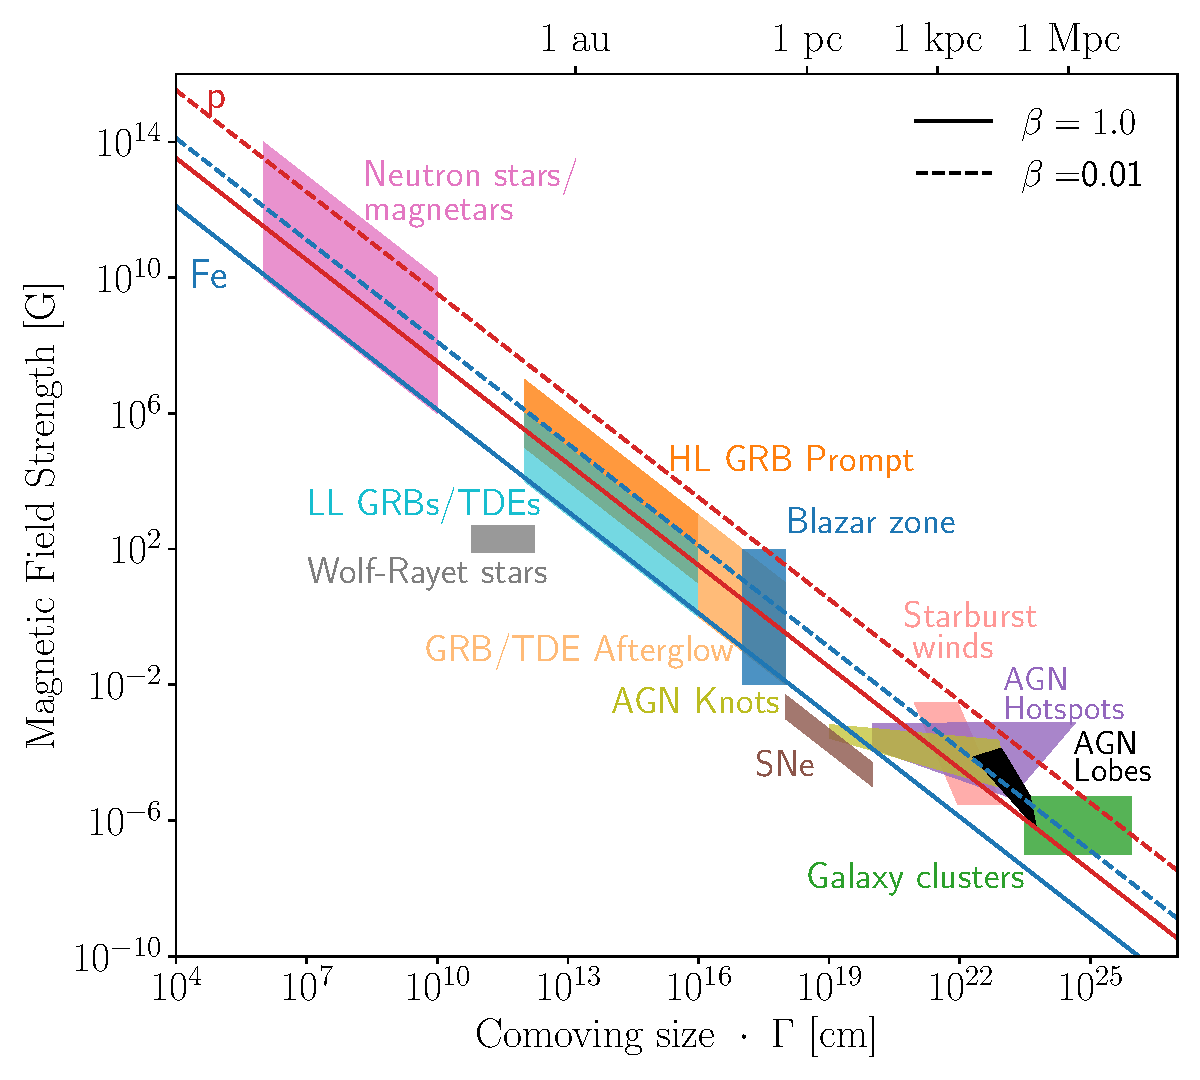
\includegraphics[width = 0.5\textwidth]{C:/Users/henri/OneDrive/Documents/NTNU/Semester 10/Masteroppgave/Plots/hillas.pdf}
    \caption{Hillas criterion for proton (blue line) and iron (red line) accelerated up to $10^{20}eV$ and $10^{21}eV$ respectively}
    \label{fig:hillas_c}
\end{figure}


\subsubsection{Macroscopic Acceleration mechanisms}
In order to accelerate particles to high energies, one needs to have a mechanism that can transfer energy to the particles. This usually happens through electromagnetic fields, and there are several ways this is thought to happen.

\textbf{One-shot acceleration}:
The simplest yet still a powerful way of accelerating particles is through what is called one-shot acceleration. In the presence of an ordered electricmagnetic fields, one can continuously accelerate charged particles which will follow the field lines. This can be induced from a rotating magnetic field or a straight electric field, all which create and electromagnetic force on a hypothetical charged particle. 
This could be the feature of some astrophysical objects such as neutron stars and black holes, usually in a quite close proximity to the object in question.% (ref cern paper)


\textbf{Second order Fermi acceleration/Diffusive acceleration}
In regions where one has high variability in the magnetic field strength, one can accelerate particles via scattering. The idea is that charged particles scatter on what can be seen as magnetic clouds and gain energy in the process due to the speed of the clouds. This mechanism is dubbed second order fermi acceleration due to the average energy gain of a particle being proportional to $(\frac{v}{c})^2$. Here $v$ is the speed of the cloud and $c$ is the speed of the particle. This is a slow process due to the proportionality to $v^2$, but as mentioned in \cite{Dermer_2001} can be a viable way of accelerating particles which already have a high energy. In modern times the magnetic mirrors that particles scatter on are thought to be plasma waves. The idea is that particles occupy a background magnetic field $B_0$ with a superimposed fluctuating electromagnetic field which arrise due to cold-plasma waves. The full formalism is described in \cite{BHradiation} at page 361. In trying to shorten the explination on only focuses on the resulting energy gain. The mean rate of change of the momentum of a particle is given as

\begin{equation}
    \left<\frac{dp}{dt}\right> = \frac{1}{p^2}\frac{\partial}{\partial p}\left[p^2D(p)\right] 
\end{equation}

where the real challenge lies in determining the diffusion coefficent $D(p)$ which is a function of the particle momentum and pitch angle. One will follow the approach found in \cite{O_Sullivan_2009} in which one only considers alfvén waves which take a one-dimensional power spectrum $W(k) \propto k^{-q}$, where $q$ is the spectral index and the total internal energy of the waves is given as $\frac{\delta B^2 }{8\pi}= \int_{k_{min}}^{k_{max}} W(k)dk$.   

As given in \cite{O_Sullivan_2009} the diffusion coefficient with current wave spectrum can be given as

\begin{equation}
    D(p) = \beta_a^2 \frac{\delta B^2}{B_0^2}\left(\frac{r_g}{\lambda_{max}}\right)^{q-1} \frac{p^2c^2}{r_g c}
\end{equation}

where $\beta_a = \frac{B}{\sqrt{4 \pi n_p m_p}c}$ is the alfvén speed, $r_g = \frac{pc}{ZeB}$ is the gyroradius of the particle, and $\lambda_{max}$ is the maximum wavelength of the waves, which will be specified when necessary, but if one is following \cite{O_Sullivan_2009} takes the value of $0.1 R$, i.e. a magnitude lower than the radius of the emitting region.

Form here one can estimate the acceleration timescale of a particle in a given region. The timescale is given as

\begin{equation}
    t_{acc} = \frac{p^2}{D(p)}
\end{equation}


\textbf{First order Fermi acceleration}
In regions where one has strong shock fronts, one can accelerate particles to high energies. These environments can be found several places where the interstellar medium is interacting with a powerful source of energy. One of the most famous examples of this is the supernova remnant where one sees a powerful shock front as a result of a supernova explosion.  
The first-order Fermi acceleration happens when particles traverse these strong shock fronts, and when a particle moves through the shock it gains energy proportional to $\frac{v}{c}$. In addition to this, there is a probability that the particle will stay in the accelerating region and 
experience several accelerations. 

In \cite{Dermer_2001} they can derive the relative power of a particle undergoing first-order Fermi acceleration in a relativistic shock, and it is given as 



\begin{equation}
    \dot p = \frac{2p}{t_u} = \frac{2cqB\Gamma}{mc^2 }
\end{equation}


where $t_u$ is the time in the upstream frame, $p$ is the momentum of the particle, $c$ is the speed of light, $q$ is the charge of the particle, $B$ is the magnetic field strength, $\Gamma$ is the Lorentz factor of the shock, and $m$ is the mass of the particle.

\textbf{KI instabilities in jets}
Another method of acceleration which really is diffusive one shot acceleration related to AGN jets is acceleration via the kink instability in jets. The idea of kink instability leading to acceleration is found in \cite{Alves_2018}. Kink instability is a hydrodynamic instability that arises in jets when the magnetic field is not aligned with the jet. If a perturbation is introduced to the jet, the resulting force on the jet structure will magnify the perturbation. This will lead the jet to a much more complicated structure, and twist the magnetic field lines. See figure \ref{fig:kink_instability} for an illustration. The paper argues that a highly tangled magnetic field and a large scale inductive electric field which is found throughout the kink-unstable region will lead to rapid energization of particles. 

\begin{figure}
    \centering
    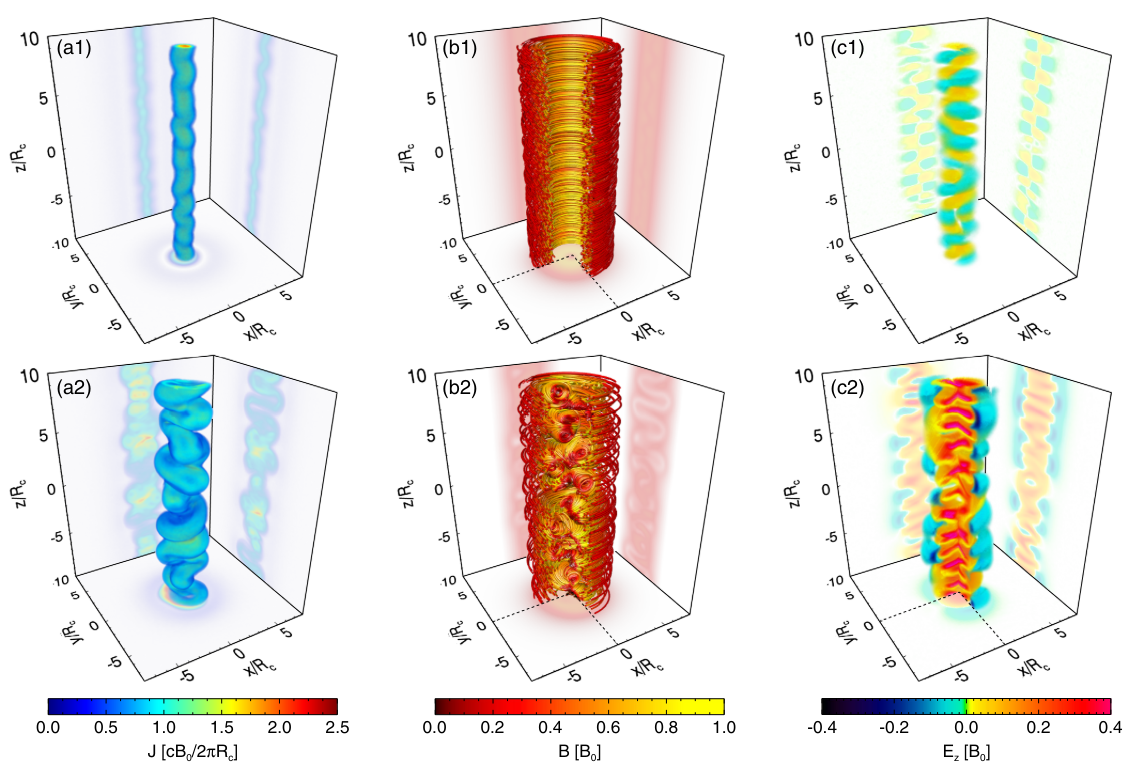
\includegraphics[width = 0.8\textwidth]{C:/Users/henri/OneDrive/Documents/NTNU/Semester 10/Masteroppgave/Plots/KI_instability.png}
    \caption{Simulations from \cite{Alves_2018} showing the evolution of kink instability in a jet. The upper panels shows the before the KI instability has been amplified, and the lower panel shows the jet after the instability has been amplified. From left to right the panels show, Current density, magnetic field lines, and axial electric field. }
    \label{fig:kink_instability}
\end{figure}

\subsection{UHECRs}

UHECRs are charged particles that are bombarding the Earth with energy exceeding 1 exaelectronvolt ($10^{18}$ eV) according to \cite{Alves_Batista_2019}. The origin of 
these particles is still a mystery but due to their high energies, they are thought to be extragalactic in origin.
The composition of UHECRs ranges from protons to heavier nuclei such as helium or iron, and when these particles interact with the atmosphere they produce a shower of secondary particles.
The air showers could also give extra information such as direction, but due to the nature of UHECRs, the location of their source is
difficult to pinpoint. This is because UHECRs are charged particles and therefore are deflected by the magnetic fields they encounter.

\subsubsection{Production and Energy loss}
The requirements to produce a UHECR are a charged particle and a powerful accelerator. But in order to
model them sufficiently one needs to take into account their journey to the Earth. Both during the acceleration and during the journey to Earth, the UHECRs will lose energy. 
The important parameters for this energy loss are its composition and its environment. In addition, as mentioned before, the interstellar magnetic field will also deflect the particles and therefore the direction of the particle will be changed. 
These effects are important parameters since they limit the 
distance a particle can travel before it loses too much energy, and therefore limits the local volume in which high energy cosmic rays can be produced. 
Here I will briefly discuss the different energy loss mechanisms.

\newpage
\chapter{Active Galactic Nuclei}
%\section{Active Galactic Nuclei}
\label{sec:AGN}






Active Galactic Nuclei (AGN) are an interesting topic in astrophysical studies, and 
since their discovery, there has been rapid advancement in understanding these phenomena.
Today, AGN are known to be among the brightest entities in the night sky,
but they only gained significant attention in the early 1950s. 
This shift occurred with the arrival of new radio observations, which revealed a new type of quasi-stellar
object through the discovery of the Quasars.

Initially, these luminous objects, characterized by broad, 
unidentifiable spectral lines, were enigmatic to scientists. 
However, with the identification of more sources and their optical parts, 
it became clear that these were not stars but a distinct class of celestial objects. 
Furthermore, research done by M. Schmidt on one of the emission lines from 
Quasar 3C 273 opened the interpretation of these celestial objects. 
He found that the emission lines of quasars were similar to hydrogen, but were redshifted by a factor of 0.158,
an exceptionally high value at the time according to \cite{Shields_1999}. Observations at the same time also revealed significant 
variability in quasar luminosity, suggesting that these objects were no larger than one light year across. 
These observations lead to the speculation of super luminous objects located very far away from Earth. The problem was that such objects
had no reasonable explanation at the time. %It was not until the mid 1960 early 1970s when modern cosmology was afoot that more of these issues were resolved.

Observation of the surrounding galaxy of AGN with matching redshift and observation of gravitational lensing cemented 
the distances of these objects. In addition, the modern view of black holes which had only been a theory in the 1950s came to
fruition and the idea of accretion allowed for the modern model of an AGN to be born. This modern perspective views AGN as supermassive black holes that
accrete matter from surrounding gas. In addition to this the modern view of AGN also include jets, torus, and different emitting regions that are used to classify AGN.

In the most recent times, a landmark achievement was achieved in March 2021, when scientists associated with the Event Horizon Telescope project 
presented the first image of the supermassive black hole at the center of the Messier 87 galaxy, located 55 million light-years away.
This image, showing a bright ring surrounding a dark central region, aligns with predictions for an accreting supermassive black hole, 
increasing our confidence in the modern model. In addition, the 2020 Nobel Prize in physics was awarded to Roger Penrose, Reinhard Genzel, and Andrea Ghez for their work on black holes, 
further cementing the importance of these objects in modern astrophysics.





\section{AGN structure and classification}


The modern view of AGN is a unified model that combines the different categories of powerful luminous objects cataloged in the mid to late 20th century. 
These distinctions that astronomers made still
have value, but to understand an AGN it is important to get a picture of the unified structure.

An active galactic nucleus is defined as a galaxy center containing a massive accreting black hole. This mass according to \cite{Netzer_2015} 
is defined as $M_{BH} > 10^5 M_\odot$. AGN also have an Eddington ratio exceeding
the limit of $L_{\rm AGN}/ L_{\rm Edd} = 10^{-5}$, where $L_{\rm AGN}$ is the bolometric luminosity, and $L_{\rm Edd}$ is the Eddington luminosity for a solar 
composition gas. These definitions help constrain what galaxies might contain an AGN, where it excludes the Milky Way 
by these criteria, but it fails to capture the full structure definition of an AGN. 
Therefore, the structure of most AGN will include several of the following components, first summarized then expanded upon: 


\begin{itemize}
    \item A close rotational dominated accretion disc around the SMBH. %The thickness defining this accretion flow will distinguish different AGN. 
    %One example is an optical thin accretion disk that sometimes becomes advection-dominated.
    %These flows will be referred to as radiation inefficient accretion flows(RIAF) due to the special nature of the disk.
   \item High-density gas clouds that are said to be dust-free moving at high velocities close to the black hole, in the so-called broad line region(BLR)
    \item Low-density gas clouds that move at lower velocities further away from the black hole in the so-called narrow line region(NLR)
    \item A structure of dust that is responsible for the obscuration of the central region of the AGN. This is called the torus due to its theorized shape. 
     It lies at a luminosity-dependent distance from the SMBH, but according to \cite{Netzer_2015} this is around 0.1 - 10 pc depending on the luminosity.
    \item A corona of hot electrons that is thought to be responsible for the X-ray emission seen in AGN. This is thought to be located above the accretion disk. 
    \item A relativistic jet that is thought to be powered by the accretion disk. This is not always present but is a common feature of AGN.
\end{itemize}

The reader is directed to figure \ref{fig:my_label} for a visual representation of the different components.


\begin{figure}
    \centering
    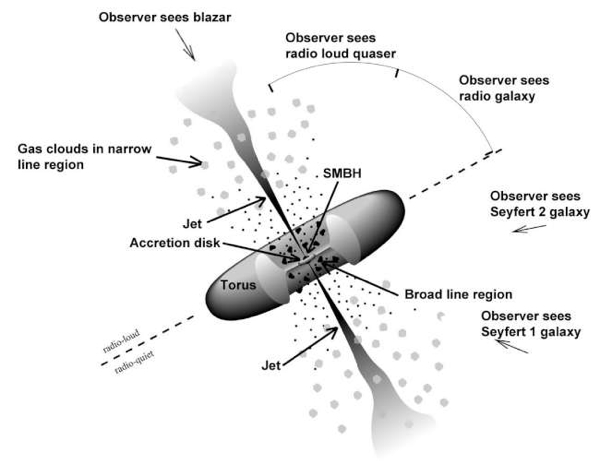
\includegraphics[width = 0.7\textwidth]{C:/Users/henri/OneDrive/Documents/NTNU/Semester 10/Masteroppgave/Plots/unified model agn.jpg}
    \caption{AGN unification}
    \label{fig:my_label}
\end{figure}

\subsection{Accretion disk}
An accretion disk is a natural consequence of the conservation of angular momentum. In the case of infalling 
matter coming close to a supermassive black hole, the matter could have some angular momentum. With this the gas should orbit the black hole at some stable distance but, due to radiative processes, fluid viscosity, and gravitational turbulence, 
the matter will lose angular momentum and spiral inwards. The inward spiral will eventually allow the matter to fall into the black hole. 
This process of inspiral is what is called accretion and the forces acting on the matter to cause the inspiral 
will also in the same process heat it up to high energies causing it to radiate. The radiation is closely linked to the 
infalling matter that is accreted onto the black hole and one can express the total luminosity of the accretion disk as 

\begin{equation}
    L_{acc} = \eta \dot{M}c^2.
    \label{eq:accretion_luminosity}
\end{equation}

Here $\eta$ is the efficiency of the accretion process, $\dot{M}$ is the mass accretion rate and $c$ is the speed of light.

%The efficiency of the accretion disk is a function of the spin of the black hole and the radius of the innermost stable circular orbit (ISCO).
%The ISCO is a counter-intuitive term in classical mechanics but in general relativity the maximum speed of a particle 
%in addition to an energy term when calculating the orbit set bounds for how close a particle can be to 
%a black hole without spiraling in. %without going into too much detail the ISCO will be a solution of this equation based on the black holes mass and spin $a$

%\begin{equation}
%    6\frac{M}{r_{ISCO}}-8\frac{aM^(\frac{1}{2})}{r^{3/2}_{ISCO}}+3\frac{a^2}{r_{ISCO}^2} = 1.
%    \label{eq:ISCO}
%\end{equation}
%It is clear from \ref{eq:ISCO} that for a non-rotating black hole the ISCO takes the radius of $6M$, the result obtained from the calculation using the Swarzschild metric.


%The accretion disk also has a bound for its maximum luminosity. As calculated for stars the Eddington
%luminosity sets a maximum strength for the radiation pressure of the accretion disk. This is given as



%\begin{equation}
%    L_{Edd} = \frac{4\pi G M m_p c}{\sigma_T}
%    \label{eq:eddington_luminosity}
%\end{equation}

The heating of the accretion disc will lead to thermal radiation from the disc and this radiation will be
proportional to the temperature of the disc. This temperature is radially dependent and if one assumes an optically thick but geometrically thin disk also called a Shakura-Sunuaev disk
one can express the radiative surface energy flux taken from \cite{BHradiation}(p. 106) as 

\begin{equation}
    \frac{dE}{dAdt}= F_{rad}(r) = \frac{3GM\dot{M}}{8\pi r^3}\left(1-\beta\sqrt{\frac{r_{\rm ISCO}}{r}}\right)
\end{equation}

Here $\beta$ is a constant that relates the fraction of angular momentum captured by the black hole, and $r_{\rm ISCO}$ is the radius of the innermost stable circular orbit. 
The temperature of the disk lie between $10^5 - 10^2$ K with emission in the optical, UV to soft X-ray range according to \cite{scholarpedia_accretion_discs}.


\subsection{Corona and X-ray emission}
From highly varying X-ray observations of AGN, it became indicative that there was a source of X-rays located close to the black hole. 
The most contemporary idea is that a corona of energetic particles is located above the accretion disk, and through inverse Compton scattering
of the optical/UV photons that arise from the accretion disk produce the seen x-ray emission. 

Inverse Compton scattering is the process of a photon gaining energy from a nearby relativistic particle. Due to the increase in efficiency 
of up scattering a photon with an electron compared to a proton, the corona x-ray emission is thought to be dominated by electrons. The process is as follows

\begin{equation}
    e^- + \gamma \rightarrow e^- + \gamma 
\end{equation}





%\subsection{Emmision lines}
%When a particle is photionized by the continuum radiation of a source it will emit a photon when it returns to its ground state. 
%This photon will have a specific wavelength that is determined by the energy difference between the two states.
%This wavelength is called the emmision line of the particle. When looking a dynamical systems with high velocities 
%the doppler shift of these emmision lines becomes important since it will affect the observed spectra of the source.

%https://lweb.cfa.harvard.edu/~pberlind/whipple/agn.html



\subsection{Broad and narrow line region}

Broad emission lines in the case of AGN are formed from the high-density gas clouds located close to the central black hole. The 
high-density parameter is inferred from the fact that one only sees broad emission from permitted line transitions (e.g. hydrogen Lyman and Balmer,
iron, and magnesium). High densities allow for collisional de-excitation and in doing so prohibit so-called forbidden transitions.
The broadening is an indication that these gas clouds are moving at huge velocities around the massive objects. This implies that they are located close to the black hole and receive the name the broad line region

Narrow emission lines are on the other hand formed in low-density gas clouds. The low densities are inferred from the fact that one sees
both permitted and forbidden line transitions. They are narrow lines due to their velocities being substantially lower than the innermost gas clouds, and from here are thought to be located further away from the black hole, in the narrow line region. 


\subsection{Dust torus}
%https://www.sciencedirect.com/science/article/pii/S0032063315000483#:~:text=This%20model%20proposes%20that%20all,collimating%20the%20radiation%20that%20escapes

The dust torus is a structure of dust that is thought to be located quite close to the black hole (0.1 - 10 pc). The main argument for the existence of this structure is the obscuration of the central region of the AGN. This obscuration 
is part of the unification scheme of AGN and was backed by the detection of polarized broad lines in AGN with their central core obscured. This polarization is what we would expect if some dust was obscuring the central region since the only light one sees is 
the light that is scattered into the line of sight according to \cite{MASON201597}. Further, the same study on the dust torus have also says that the torus is not uniform but clumpy and quite dynamic with both in and outflows of matter depending on the state of the central engine. 





\subsection{Jets}
\label{sec:jets}

A jet is a highly collimated outflow of plasma. The origin of the plasma is thought to be the accretion disk and the hot corona above it. These regions that have a high density of charged particles will under the influence of a magnetic field be accelerated and collimated into a jet-like structure.
The energy mechanism which powers the jet is not fully understood, but the most prevalent theory is the Blandford-Znajek process. It says that the rotation of the accretion disk induces a magnetic field that will interact with a rotating black hole, effectively extracting energy from the black hole and supplying it to the jet. 
The jet structure extends far beyond the local area of the AGN maintaining a stable configuration over these distances. The classification of these jets is usually divided into two groups according to \cite{walg2013relativistic}, FRI and FRII. They are differentiated by their luminosity where FRI jets are less luminous and have a more diffuse structure while FRII jets are more luminous and have a more stable structure reaching further out.
To add to this distinction it is thought that FRII jets are a product of an efficient accretion disk while FRI jets are a product of an inefficient accretion disk. This is discussed in \cite{Wei-Hao_2003} where they show that radio quiet and Seyfert 1 galaxies have lower accretion efficiency while radio loud galaxies have higher accretion efficiency. 
Beyond the energy and their structure, the jets are also notable for their emission of non-thermal radiation such as synchrotron and inverse Compton radiation. %Lastly, due to their ability to accelerate particles they are also thought to be a possible source of UHECRs and neutrinos.







\section{Types of AGN}

Before the unification of the AGN astronomers named the puzzling objects based on their observational properties. These 
names are still used to this day and are useful since their observational properties are important parameters for further study. 
The different classifications are important in understanding which objects could have the potential to produce the different observables one 
looks for in the night sky. Therefore, it seems appropriate to
discuss some different types of AGN and their observational properties. The classification in this section is heavily based on \cite{Astrobites}.

\textbf{Type I and II AGN}:
One distinguishes type I and type II AGN based on the presence of broad emission lines. In other words, this distinction is
a matter of a visible nucleus or not. Type I refers to sources whose nucleus is exposed to the observer and whose spectrum
has both narrow and broad emission lines. Type II refers to sources whose nucleus is obscured by a torus and therefore mainly has narrow emission lines.

\textbf{Blazars}:
The most extreme class of AGN. These sources are distinguished by their relativistic jets that are pointed towards the observer. 
This jet produces both synchrotron and Inverse Compton gamma rays and are extremely variable over short timescales. The
emission is also highly polarized. Often and including in this report one divides Blazars into subgroups based on the 
emission lines. The two most common are BL Lacs and Flat spectrum radio quasars (FSRQs). The difference between the two is the
presence of broad emission lines, where BL Lacs have no broad emission lines while FSRQs do. 
In addition, the distinction comes from the type of jet structure thought to be associated with the source. FRI jets for Bl Lacs and FRII for FSRQs. 

\textbf{Radio galaxies}:
Jetted AGN that as the name suggests are very bright in the radio band. They usually refer to AGN viewed edge-on, where the
torus might block the emissions from the accretion disk. The orientation of Radio galaxies gives way to strong 
synchrotron radiation, and they are often used to study the jet structure of AGN. 

\textbf{Seyfert galaxies}:
Spiral galaxies that have a bright nucleus. They are bright in the optical band and have a smaller active region 
than radio galaxies. They are often divided into two groups Seyfert I and Seyfert II where the distinction comes from type I and II. 
The galaxies also show quite high variability indicating a small emitting region. 

\textbf{Compton thin AGN}: 
A way of distinguishing AGN that can be quite useful. These AGN have lower absorption compared to Compton-thick AGN, which allow more X-rays to escape making them easier to identify. 

\textbf{Compact symmetric objects}:Compact symmetric objects were thought to be a subclass of radio galaxies that previously were thought to be young radio galaxies, but recent studies have shown that they are a distinct class of AGN and the main topic of this thesis, more on them in section \ref{sec:CSO}.

%https://iopscience.iop.org/article/10.1086/305813/fulltext/37493.text.html#:~:text=,line%20time%20delays%2C%20or%20lags


All these different distinctions are a help in understanding what processes one might be observing. The different
dominant bands indicate different processes being in the line of sight, and by considering the modern structure of 
AGN one can then try to determine the underlying dynamics.  

\newpage

\chapter{Probing Hadronic acceleration sources}
%\section{Probing hadronic acceleration sources}
%In this section one will look at different observables and methods of probing extra galactic sources as potential candidates for the origin of the UHECRs and/or neutrinos. The goal is to constrain our list of candidates by applying known effects and theoretical models to observed data. In brief one will be discussing, The hillas criterion, the anisotropy of the UHECRs and neutrinoes, "the emissivity of our sources in UHECRs and neutrinos", and a comprehensive time scale analysis of the sources.
This section outlines some different methods and observables used to probe hadronic accelerators as potential candidates for the origin of the UHECRs and/or neutrinos. The goal is to constrain our list of candidates by applying known effects and theoretical models to observed data, and to discuss the implications of these constraints. In brief, we will be discussing the density of sources, the spectral energy distribution, the magnetic field constraints, and a time scale analysis used to estimate the maximum energy attainable by ions.

\section{Density of sources}
\label{sec:prevalence_of_sources}

Due to the seemingly isotropic distribution of extra-galactic UHECRs, especially at semi-low energies as discussed in section \ref{sec:high_energy_particles} one can put limits on the density of sources. In \cite{ThePierreAugercollaboration_2013} they quote a density larger than $(0.06-5) 10^{-4} \rm{Mpc^{-3}}$ at a $95\% $ confidence level. This density, although not exceedingly large, would still dampen the idea of singular but powerful sources. Therefore, for any source to be considered, one needs to consider its density as well. 

To calculate the density of sources in the Universe there are several methods. The most common method for sources such as AGN is to use the luminosity function (LF) of the source.
The luminosity function is a function that describes the number of sources per unit volume and luminosity. Typically, the focus is on the differential luminosity function, which is defined as
\begin{equation}
    \frac{d\Psi(L,z)}{dL} = \frac{d^2N(L,V_c(z))}{dLdV_c(z)}.
\end{equation}

One also can change the differential of the comoving volume into a term only depending on the redshift assuming the source population is spread isotropically and by multiplying with the differential comoving volume element. This 
transformation goes as follows, 

\begin{equation}
    \frac{d^2N(L,V_c(z))}{dLdV_c(z)}\frac{dV_c(z)}{dz} = \frac{N(L,z)}{dLdz}.
\end{equation}

To effectively determine the LF, it's typical to divide it into two distinct components: a local term and a time evolution term.
This approach involves taking the local luminosity function, calculated at a redshift 
$z=0$, and then scaling it with a function that accounts for the change in redshift. 
The exact form of the total LF varies based on the source object, but it generally falls into two categories derived from the method of incorporating the growth term into the local LF.
These methods are selected based on which best represents the observed evolution.

The two distinctions are the Pure Density Evolution (PDE) and the Pure Luminosity Evolution (PLE). 
The PDE model modifies the local density function to reflect changes over time, 
while the PLE model adjusts the local luminosity. The evolution is better represented by their equations and is given as 

\begin{equation}
\frac{d\Psi(L,z)}{d(L)} = 
    \begin{cases}
        \frac{d\Psi(L/e(z),z=0)}{d(L)} \quad (PLE)\\
        \frac{d\Psi(L,z=0)}{d(L)}e(z) \quad (PDE)\\
    \end{cases} .
\end{equation}

For some sources which lack observational data, it can be difficult to estimate a full luminosity function. Due to the lack of observation or a big bias in the catalogue selection, different sources are not constrained enough and therefore one must rely on simpler estimates of their densities. One such method given that the lifetime of a source is known is via probability. The density is estimated by calculating the required density one needs to produce the observed amount of sources, or in the worst case one source given its average lifetime. This will in most cases serve as a lower limit, and give us a starting point for further analysis.  

In order to do so, one defines the probability of seeing a source that has a lifetime $t_l $ up to a horizon $t(z)$ as 

\begin{equation}
    p = \frac{t_l}{t(z)}.
\end{equation}
The horizon is the redshift at which one stops finding appreciable number of the source. The required density such that one observes a source at present time can then be estimated as 

\begin{equation}
    n = \frac{1}{p V(z)} 
\end{equation}

Where $V(z)$ is the comoving volume of the Universe up to the horizon.
The calculation is crude, but allows us to make lower limit estimates on sources where the Luminosity function is not defined. An example of this is seen in section \ref{sec:prevalence} where we estimate the density of CSOs.


\section{SED broad band analysis}
The spectral shape of emitting galaxies and galaxy cores tells us a lot about the underlying dynamics, and with this information we can start to peel away the complex layers. The spectral energy distribution (SED) of a source is a plot of the photon energy emitted by the source as a function of frequency. In Figure \ref{fig:AGN_SED} one can see a model of a typical SED of an AGN in which the jet components, that is to say the synchrotron and inverse Compton components, are not dominant. The different components of the AGN are visible in the plot, and understanding how different components are created and contribute to the nearby environment will give us a better understanding of what observables we might expect from sources such as these. The following section will outline the different components of the SED and how they are modelled.

\begin{figure}
    \centering
    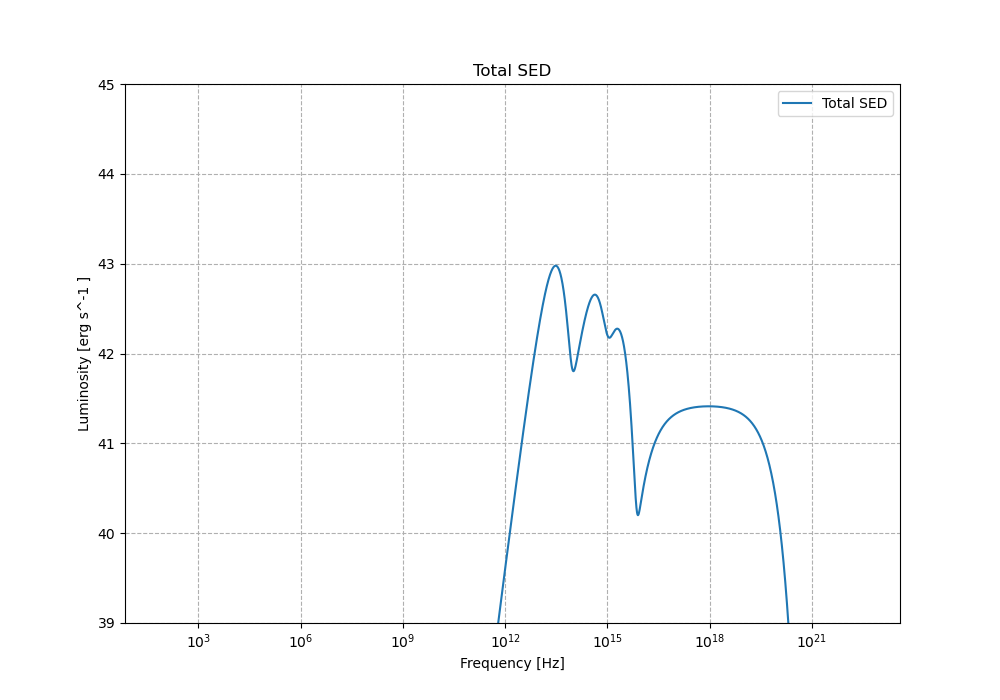
\includegraphics[width=0.9\textwidth]{C:/Users/henri/OneDrive/Documents/NTNU/Semester 10/Masteroppgave/Plots/SED.png}
    \caption{The spectral energy distribution of an AGN viewed without beaming from the jet. The different components of the AGN are visible in the plot.}
    \label{fig:AGN_SED}
\end{figure}

%\subsection{X-ray energy budget}
%The X-ray energy budget of especially Active galactic nuclei is often used as a probe for UHECRs and neutrino emissivity. This makes the X-ray Luminosity of AGN an interesting parameter that warrants further analysis. In this sense the X-ray luminosity is often used a proxy for the total energy budget of escaping particles, but a true relation between the two is not known. The X-ray luminosity of an AGN usually has two sources of emission, the corona, and IC scattering of the synchrotron radiation in the jets. In both cases the main mechanism is thought to be Inverse Compton scattering and for that one requires relativistic electrons. Requiring relativistic electrons is a good indicator that there might be relativistic protons present as well, and following that logic one can start to estimate the energy budget of the protons. 

%\subsection{Radio luminosity}
\subsection{Core photon fields around AGN}
\label{sec:photon_fields}

In order to determine the photon fields around AGN cores we follow \cite{Ghisellini_2009} which describes the photon fields surrounding a Blazar. The photon fields separate into different contributions from the different regions of a classic AGN as discussed in section \ref{sec:AGN}. 
The different core regions of an AGN are the accretion disk, the broad line region, the torus, and the X-ray corona. 

\textbf{Accretion disk:} The photon field emerging from an accretion disk is calculated by assuming a black body spectrum at each ring of a Shakura-Sunyaev disk and summing up its contributions. The temperature of 
each ring in the disk is given by 

\begin{equation}
    T(R) = \left(\frac{3 R_{S} L_{d}}{16 \pi R^3 \eta \sigma_{\mathrm{SB}}} \left(1-\left(\frac{3 R_{S}}{R}\right)^{\frac{1}{2}}\right) \right)^{\frac{1}{4}}
\end{equation}

Each ring of the accretion disk is assumed to be emitting as a black-body spectrum, which is defined as

\begin{equation}
    \label{eq:BB}
    I(\nu) = \frac{2 h \nu^3}{c^2} \left(\frac{1}{\exp\left(\frac{h \nu}{k_B T}\right) - 1}\right).
\end{equation}

By integrating the intensity over all annuli of the disk we can find the total flux of the disk and from there the total energy density of the disk per frequency.

The resulting spectral energy density as seen in the comoving frame of an observer at $R$ is then given by

\begin{equation}
    u_d'(\nu') = \frac{2\pi}{c} \int_{\mu_d}^1 I'(\nu')\delta^{-2} d\mu
\end{equation}
where $\mu_d$ is the cosine of the angle between the location on the disk and the normal of the disk with respect to the observer, and $\delta = \Gamma(1-\beta \mu)$ is the Doppler factor. 

\textbf{X-ray corona:} The photon field from the X-ray corona is assumed to be a power law spectrum with a cut off at high energies. Its total energy emitted is related to the disk luminosity 
by the equation $L_{cor} = f_X L_d$ where $f_X$ is the fraction of the disk luminosity that is emitted by the corona. The spectral energy density of the corona is then given by 

\begin{equation}
    U_{cor}(\nu) = D(R)\left(\frac{\nu}{\nu_0}\right)^{-\alpha} \exp\left(-\frac{\nu}{\nu_{cut}}\right)
\end{equation}

The factor $D(R)$ is a scaling factor that incorporates the position of the observer. The integral of the spectral energy density over all frequencies should equate to the total energy density in X-ray at the location of the observer.

The energy density of X-ray around the central engine is given by

\begin{equation}
    \text{UX'}(R) = \frac{f_{X} L_{d} \Gamma^2}{\pi (R_{X})^2 c} \left(1 - \mu_{X} - \beta(1 - \mu_{X}^2) + \frac{\beta^2 (1 - \mu_{X}^3)}{3}\right)
\end{equation}
where
\[
\mu_{X} = \left(1 + \frac{R_{X}^2}{R^2}\right)^{-0.5}.
\]

Here $f_{X}$ is the fraction of the disk luminosity that is emitted by the X-ray corona, $L_{d}$ is the disk luminosity, $\Gamma$ is the Lorentz factor of the jet, $R_{X}$ is the size of the X-ray corona, $\beta$ is the velocity of the observer in units of the speed of light.
In short, the X-ray energy density stays constant until the observer is further away where it will decrease as $1/R^2$ which is to be expected.

\textbf{Broad line region:} The broad band field is assumed to be emitting a black body spectrum as in equation \ref{eq:BB} which peaks at the Lyman-alpha line. The Lyman-alpha line is a spectral line of hydrogen when the atomic electron transitions from the $n=2$ to the $n=1$ orbital.
Similarly to the X-ray corona, the spectral energy density is scaled to the region of interest and the total energy density as a function of distance is given by: 

\begin{equation}
    \label{eq:UBLR}
    \text{UBLR'}(R) = 
    \begin{cases}
    \frac{17}{12}\frac{f_{\text{BLR}} L_{d} \Gamma^2}{4\pi R_{\text{BLR}}^2 c} & \text{if } R \leq R_{\text{BLR}}, \\
    \frac{f_{\text{BLR}} L_{d} \Gamma^2}{4 \pi R_{\text{BLR}}^2 c \beta 3} \left[2 (1 - \beta \mu_{\text{IR1}})^3 - (1 - \beta \mu_{\text{IR2}})^3 - (1 - \beta)^3\right] & \text{if } R \geq 3R_{\text{BLR}}, \\
    a R^b & \text{otherwise},
    \end{cases}  
\end{equation}
where 
\begin{align*}
    \mu_{\text{IR1}} &= \left(1 + \frac{R_{\text{BLR}}^2}{R^2}\right)^{-0.5}, \\
    \mu_{\text{IR2}} &= \left(1 - \frac{R_{\text{BLR}}^2}{R^2}\right)^{-0.5}, \\
    %b &= \log\left(\frac{\text{UBLR}(3R_{\text{BLR}}, R_{\text{BLR}}, f_{\text{BLR}}, L_{d}, \Gamma)}{\text{UBLR}(R_{\text{BLR}}, R_{\text{BLR}}, f_{\text{BLR}}, L_{d}, \Gamma)}\right) / \log(3), \\
    %a &= \frac{\text{UBLR}(R_{\text{BLR}}, R_{\text{BLR}}, f_{\text{BLR}}, L_{d}, \Gamma)}{R_{\text{BLR}}^b}.
\end{align*}

\textbf{Torus:} There is also assumed to be a dusty torus around the AGN emitting in infrared. The spectral energy density of the torus is also given by 
a black body spectrum given in equation \ref{eq:BB}. The total energy density of the torus has the same relations 
as the BLR for $R>R_{IR}$ but with the relevant parameters for the torus. For $R<R_{IR}$ the energy density is given as

\begin{equation}
    \text{UIR'}(R) = 
    \begin{cases}
    \frac{f_{\text{IR}}L_d \Gamma^2}{4 \pi R_{\text{IR}}^2 c} & \text{if } R \leq R_{\text{IR}}, \\
    \end{cases}
\end{equation}

\subsection{Non-core photon fields}
\label{sec:non_core_photon_fields}
In addition to the core photon fields we will model the photon field from relativistic electrons occupying a magnetic field, i.e. Synchrotron radiation, Synchrotron self Compton radiation, and Inverse Compton radiation of the core fields. The information and derivation of these subsections are taken from \cite{BHradiation}. We note lastly that all calculations below are done in the comoving frame of the source, and one must transform the results to the observer frame if one wishes to estimate observed flux quantities.

\begin{figure}
    \centering
    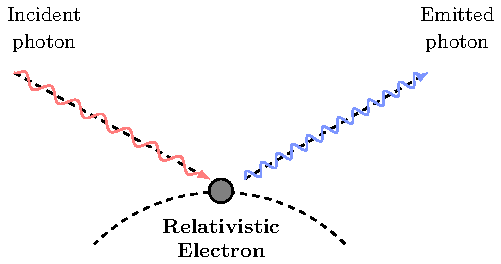
\includegraphics[width=0.7\textwidth]{C:/Users/henri/OneDrive/Documents/NTNU/Semester 10/Masteroppgave/Plots/Inverse_compton.pdf}
    \caption{The inverse Compton scattering process. The process is the scattering of a low energy photon by a relativistic electron. The scattered photon will have a higher energy than the original photon. Image taken from \cite{BennumAlfred}}
\end{figure}

\textbf{Synchrotron radiation:} 
\label{sec:synchrotron_radiation}
For a given population of relativistic electrons that occupy energies between $\gamma_{min}$ and $\gamma_{max}$ in a magnetic field $B$, the movement of the electrons through the magnetic field will cause them to spiral, and in turn emit synchrotron radiation. For relativistic particles at pitch angle $\pi/2$ to the magnetic field, the spectral energy radiated per revolution at $\omega = 2\pi \nu$ around the magnetic field is given by

\begin{equation}
    I(\omega) = \frac{2 e^2 \omega}{\sqrt{3}\gamma^2 \omega_L c} \int_{2\omega/3\omega_L\gamma^2 }^{\infty} K_{5/3}(\xi)d\xi  
\end{equation}

where $\omega_L = eB/mc$ is the Larmor frequency.

The radiated power at the frequency $\nu$ is $P(\nu) = 2\pi P(\omega) = \omega_L I(\omega)$ which allows us to write the power radiated by an electron at frequency $\nu$ as

\begin{equation}
    P(\nu) = \frac{\sqrt{3} e^3 B}{m c^2} \left(\frac{\nu}{\nu_c}\right) \int_{\nu/\nu_c}^{\infty} K_{5/3}(\xi)d\xi = \frac{\sqrt{3} e^3 B}{m c^2} F\left(\frac{\nu}{\nu_c}\right)
\end{equation}

where $\nu_c = \frac{3\gamma^2}{2}\left(\frac{eB}{2\pi m_e c}\right)$ is the critical frequency.

We will now skip a few steps for brevity, but if one is interested, one can find the full derivation in \cite{BHradiation} on page 126. Then for a distribution $N(\gamma)$ of electrons where the average distribution of electrons is static, and averaged over all pitch angles we can write the total power radiated as

\begin{equation}
    P(\nu) = \frac{\sqrt{3} e^3 B}{m c^2} \int_{\gamma_{min}}^{\gamma_{max}} N(\gamma) R\left(\frac{\nu}{\nu_c}\right)d\gamma
\end{equation}

where 

$$
R(\nu/\nu_c = x) =  \frac{x}{2} \int_0^\pi d\theta \sin\theta \int_{x/\sin(\theta)}^{\infty} K_{5/3}(t)dt
$$
\begin{equation}
    = \frac{1}{2}\pi x(W_{0,\frac{4}{3}}(x)W_{0,\frac{1}{3}}(x)-W_{\frac{1}{2},\frac{5}{6}}(x)W_{\frac{-1}{2},\frac{5}{6}}(x))
\end{equation}
Here the $W$ functions are the Whittaker functions, these are defined in the appendix. 

In addition to emitting synchrotron radiation, the same electrons can also absorb the radiation. This is called synchrotron self-absorption, and the relation between the full synchrotron power and the observed synchrotron power for a sphere due to self-absorption is

\begin{equation}
P(\nu)_{\text{SSA}} = P(\nu)_{\text{syn}}\frac{3 u(\tau_{\nu})}{\tau_{\nu}}
\end{equation}
where $\tau_{\nu} = 2 \kappa_{\nu} r_b$ is the frequency-dependent optical depth, and 
$u(\tau_{\nu}) = \frac{1}{2}\left(1- \frac{2}{\tau^2}[1-(1+\tau)\exp{-\tau}]\right)$. The parameter of interest is the frequency-dependent self-absorption coefficient $\kappa_{\nu}$ which can be estimated via a delta approximation as 

\begin{equation}
    \kappa_{\nu, approx} = -\frac{\pi}{36} \cdot \frac{c r_e}{\nu} \left[\gamma^2 \frac{d}{d\gamma}\left(\frac{n(\gamma)}{\gamma^2}\right) \right]_{\gamma = \sqrt{\frac{\nu}{2 \nu_B}}}
\end{equation}

where $\nu_B = \frac{e B}{2 \pi m_e c }$ is the critical frequency of the magnetic field.

\textbf{Synchrotron self Compton radiation:}
In addition to radiating synchrotron radiation, non-thermal electrons also have the ability to Compton scatter on the same radiation that they emit. This radiation is called synchrotron self Compton radiation (SSC). In order to calculate the resulting radiation, We must first calculate the energy density of the synchrotron radiation. For a given sphere of emitting electrons, the average energy density of the synchrotron radiation is given as

$ u(\nu) = \frac{1}{4 \pi R^2 c} P(\nu) $
    
We again skip some steps and define the SSC luminosity as

\begin{equation}    
\epsilon_s J_{\text{SSC}}(\epsilon_s) =  \frac{3}{4} \sigma_T c \epsilon_s^2 \int_0^{\infty} d\epsilon \frac{u_{\text{syn}}(\epsilon)}{\epsilon^2} \int_{\gamma_{min}}^{\gamma_{max}} d\gamma \frac{N_e(\gamma)}{\gamma^2} F_C(q,\Gamma)
\end{equation}

where $\sigma_T$ is the Thomson cross section, $\epsilon_s$ is the energy of the SSC photon in dimensionless units: $\epsilon = \frac{h\nu}{m_e c^2}$, $u_{\text{syn}}$ is the energy density of the synchrotron radiation, $N_e$ is the electron distribution, and 

$$
F_c = \left(2q\ln (q) + (1+2q)(1-q) + \frac{1}{2}\frac{\Gamma q}{1+ \Gamma q}(1-q)\right)\times H\left(q; \frac{1}{4\gamma^2},1\right),
$$
$$
q = \frac{\epsilon_s}{\gamma \Gamma(1-\epsilon_s/\gamma)}, \quad \Gamma = 4\gamma \epsilon
$$

\textbf{Inverse Compton radiation:}

The last photon field to study is the inverse Compton radiation, which is similar to the SSC radiation but instead of scattering on the synchrotron radiation, the electrons scatter on the photon fields from the core. The biggest difference here is the angular dependency on the incoming photon field. For SSC we assumed that the synchrotron radiation was isotropic, but for IC we must take into account that the radiation comes from a narrow angle. For simplicity, we assumes that the external photon density follows this distribution 

\begin{equation}
    u_{ext}(\epsilon,\theta) = K u_{ext}(\epsilon)(1-\cos \theta)^4  
\end{equation}

where $K$ is a normalization constant. We then give the luminosity of the IC radiation as

\begin{equation}
    \epsilon_s J_{\epsilon}^{\text{EC}} = c \pi r_e^2 \epsilon_s^2 \int d\Omega \int_0^{\epsilon_{ext}^{\text{high}}} d\epsilon_{ext} \frac{u_{ext}(\epsilon_{ext}, \Omega)}{\epsilon{_ext}^2} \int_{\gamma_{\text{low}}}^{\infty} d\gamma \frac{N_e'(\gamma)}{\gamma^2} \Xi_C.
\end{equation}

where $r_e$ is the classical electron radius, $\epsilon_s$ is the energy of the IC photon, $u_{ext}$ is the energy

\section{Magnetic field constraints}
For acceleration in astrophysical sources one usually requires a relatively strong magnetic field. In this section, we will outline some methods for estimating the magnetic field strength in astrophysical sources based on their radio observations, namely the equipartition method and the synchrotron self-absorption method.

\subsection{Equipartition}
\label{sec:equipartition}
The most well-known estimate for magnetic field strength in astrophysical sources is through the equipartition argument. The fact that we observes synchrotron radiation implies that a source of relativistic electrons with energy density $U_e$ 
possess a magnetic field with energy density $U_B$. The question that one aims to answer with the equipartition argument is what is the minimum total energy in both relativistic particles and magnetic fields required to produce the observed synchrotron radiation of a given frequency. The total energy in relativistic particles and magnetic fields of a volume $V$ is given as

\begin{equation}
    U_{tot} = U_p + U_B = V(u_p + u_{mag})
\end{equation}

Here $u_p$ is the energy density of all relativistic particles, i.e., electrons, protons, and heavier ions ($Z>1$). Ions emit very little synchrotron radiation for a given energy $E$ compared to electrons, so little is known about their energy density; therefore, it is common to assume

\begin{equation}
    u_p = \eta u_e
\end{equation}

where $\eta$ is a constant $>1$ and $u_e$ is the energy density of the relativistic electrons. In order to estimate the energy density of the electrons, we assumes their distribution as a power law $n(E) \propto E^{-\delta}$, and their energy density becomes

\begin{equation}
    u_e = \int_{E_{min}}^{E_{max}} n(E) E dE = K \int_{E_{min}}^{E_{max}} E^{1-\delta }dE
\end{equation}

The radiated power of an electron peaks strongly around the critical frequency $\nu_c$, and following \cite{2013Wilson} Chapters 10.8 and 10.10, we can then write a relation between a frequency $\nu$ and energy $E$ as

\begin{equation}
    \nu = \frac{3}{2}\frac{eB}{m_e^3 c^5}E^2.
\end{equation}

This allows for the particle energy density to be written as

\begin{equation}
    \label{eq:energy_density_particles}
    u_p = K \frac{\eta}{1-2n} \left(\frac{e}{m^3c^5}\right)^{n-1/2}\left(\nu_{max}^{1/2-n}-\nu_{min}^{1/2-n}\right) B^{n-1/2} = K G B^{n-1/2}
\end{equation}
by introducing the constant $n = \frac{1}{2}(\delta -1 )$. 

The energy density of the magnetic field is given as

\begin{equation}
    u_{mag} = \frac{B^2}{8\pi}
\end{equation}

To move further, one wishes to eliminate the factor $K$ from our equations and relate it to observed properties. \cite{2013Wilson} gives the emissivity of a synchrotron source for tangled magnetic fields as

\begin{equation}
    \epsilon(\nu) = b(n)K \frac{e^3}{m c^2}\left[\frac{3 e}{4 \pi m^3 c^5}\right]^{n} B^{n+1} \nu^{-n} = H K B^{n+1} \nu^{-n},
\end{equation}

where $b(n)$ is a function of the spectral index $n$ given in the appendix. The observed flux density of a source with volume $V$ and at distance $R$ is given as

\begin{equation}
    \label{eq:flux_density_eq}
    S(\nu) = \frac{V}{R^2} \epsilon(\nu) \propto B^{n+1} \nu^{-n}
\end{equation}

Using this relation, we can then write the total energy density while inserting equation \ref{eq:flux_density_eq} as $K$ in equation \ref{eq:energy_density_particles} as

\begin{equation}
    U_{tot} = \frac{G}{H}R^2(S_v\nu^n)B^{-3/2} + \frac{V B^2}{8\pi}
\end{equation}

One then argues that $U_{tot}$ should have a minimum value, and given that we has measurements on distance, volume, and flux density, we can then estimate the magnetic field strength. The magnetic field strength will then be

\begin{equation}
    B_{eq} = \left(\frac{6\pi G}{H}\frac{R^2}{V}S_\nu \nu^n\right)^{2/7}
\end{equation}
This relationship between $U_B$ and $U_e$ at this minimum is very near the equipartition value, which is why this method is often called as such.


\subsection{Synchrotron self absorption}
\label{sec:SSA}

The theory of synchrotron self-absorption is a tool used previously for estimating magnetic field strength in spherically symmetric synchrotron sources. Synchrotron self-absorption is the process where the synchrotron radiation is absorbed by the same electrons that produced it as seen in section \ref{sec:synchrotron_radiation}, and the effect of this is that any given volume of emitting plasma that radiates synchrotron radiation will have a frequency below which the plasma is opaque. This frequency at which this happens is called the turnover frequency, and one aims to show how one can estimate the magnetic field strength in the emitting plasma based on this shape of the spectrum at this frequency. The concept was first introduced by \cite{1983ApJ...264..296M}, but this section relies heavily on \cite{Hirotani_2005} for the derivation. 

%Before we begin the derivation it is fitting to understand the spectrum of synchrotron radiation from a plasma. The spectrum is characterized by the peak frequency, also called the turnover frequency $\nu_m$, the peak flux density $S_m$, and naturally the spectral index $\alpha$. One referse the reader to image \ref{fig:synchrotron_spectrum} for a simple view of the synchrotron speaktrum in question. 

\begin{figure}
    \centering
    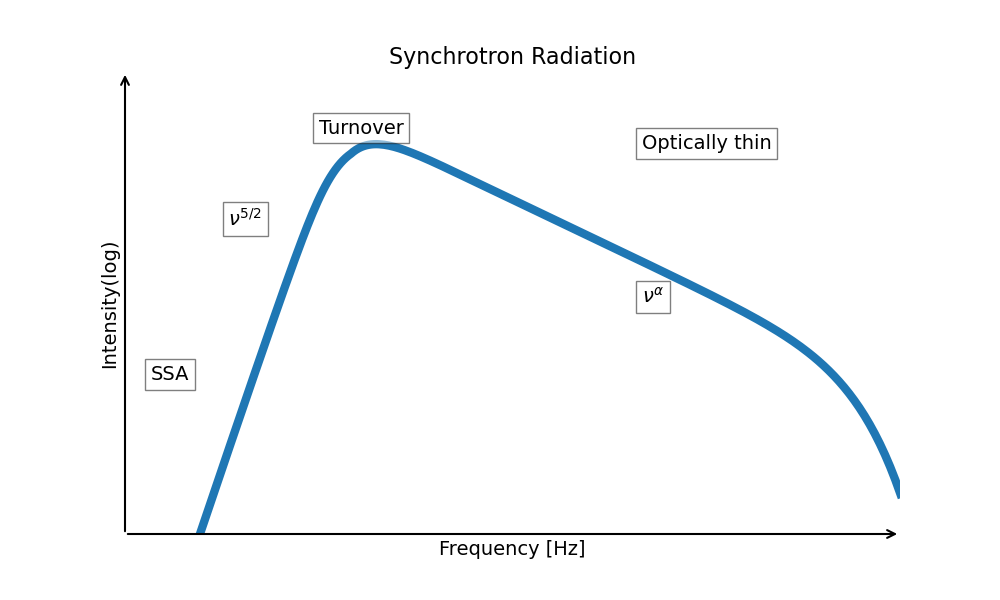
\includegraphics[width=0.75\textwidth]{C:/Users/henri/OneDrive/Documents/NTNU/Semester 10/Masteroppgave/Plots/Synchrotron_radiation.png}
    \caption{Typical synchrotron spectrum of a Giga hertz peaked galaxy (GHP). Later on we will see that GHP galaxies and CSO occupy the same niche. Image similar to one from Group of Active Galactic Nuclei investigation at https://www.sao.ru/hq/giag/gps-en.html }
    \label{fig:synchrotron_spectrum}
\end{figure}

In order to estimate the magnetic field strength we must assume that it is uniform and that the electron density is also uniform. From here the transfer equation for escaping synchrotron radiation is given in \cite{Hirotani_2005} and the specific intensity can be written as 

\begin{equation}
    I_\nu = A(\alpha) \nu^{'\frac{5}{2}}[1-\exp(-\alpha_{\nu}'x_0' )] 
\end{equation}
where 

\begin{equation}
    A(\alpha) = \frac{3}{2}^{-\alpha}\frac{e}{c}\frac{a(\alpha)}{C(\alpha)}\left(\frac{e}{2\pi m_e c}\right)^{-3/2}B^{-1/2}
\end{equation}

where $x_0'$ is the thickness of the emitting plasma along the observer's line of sight. The coefficients $a(\alpha)$ and $C(\alpha)$ are tabulated values that depend on the spectral index $\alpha$, not to be confused with the absorption coefficient $\alpha_{\nu}$, and any value denoted with a $'$ is in the comoving frame. 

Imagining an observer at a distance $D$ with angle $\theta$ from the blob of plasma (as seen in Figure \ref{fig:Radiative_transfer}), one can define the fractional thickness, which is a Lorentz-invariant quantity, as

\begin{equation}
    \frac{x_0'}{2R'} = \cos(\theta + \xi) = \sqrt{1-\left[\frac{\sin(\theta)}{\sin(\theta_d/2)}\right]^2}
\end{equation}

Determining that $\tau(0) \equiv  \alpha'2R'$ is the optical depth for $\theta = 0$, one can then get the full specific intensity as

\begin{equation}
    I_\nu(\theta) = \left( \frac{\delta}{1+z}\right)A(\alpha)\nu^{\frac{5}{2}}\left(1-\exp \left(-\tau(0)\sqrt{1-\left[\frac{\sin(\theta)}{\sin(\theta_d/2)}\right]^2}\right)\right)
\end{equation}

The shape of the blob is assumed to be spherical, and one can integrate the specific intensity over the entire blob to get the total flux density as

\begin{equation}
    \label{eq:flux_density}
    S_\nu = 2\pi \int_0^{\theta_d/2} I_v(\theta)\cos(\theta)\sin(\theta) = \pi \sin^2(\frac{\theta_d}{2})(\frac{\delta}{1+z})^{1/2}A \nu^{5/2} \int_0^1[1-\exp(-\tau(0)\sqrt{1-x^2})]dx
\end{equation}
where $x \equiv \left[\frac{\sin(\theta)}{\sin(\theta_d/2)}\right]^2$.
Here we insert what we know about the synchrotron spectrum and the turnover frequency $\nu_m$, notably that the derivative is zero at $\nu_m$. We derive the flux density with respect to frequency and set it equal to zero to find the equation that relates $\tau_\nu(0)$ and $\alpha$ at the turnover frequency. In order to do this, one needs to know the relation between the absorption coefficient and frequency. This is given also in \cite{Hirotani_2005} as 
\begin{equation}
    \alpha_\nu' = C(\alpha) r_e^2 k_e^*\frac{\nu_0}{\nu'}(\frac{\nu_B}{\nu'})^{(-2\alpha +3)/2}
\end{equation} 

where $\nu_e \equiv c/r_e$ is the electron frequency, $r_e \equiv e^2/(m_e c^2)$, and  
$\nu_B \equiv eB/(2\pi m_e c)$ is the cyclotron frequency. 

Having the solution for $\tau_\nu(0)$ as a function of $\alpha$, we denotes the solution at the turnover frequency as $\tau_m(0)$. This is a tabulated value and the table from \cite{Hirotani_2005} is found in the appendix.

Using this solution, we can inversely solve equation \ref{eq:flux_density} for the magnetic field strength $B$ and obtain with the small angle approximation 

\begin{equation}
    B =   10^{-5} b(\alpha) \left(\frac{S_m}{\text{Jy}}\right)^{-2}\left(\frac{\nu_m}{\text{GHz}}\right)^{5}\left(\frac{\theta_d}{mas}\right)^{4}\left(\frac{\delta}{1+z}\right) \text{G}.
\end{equation}
Here $\theta_d$ is the angular diameter of the source given in milliarcseconds(mas), and $S_m$ is the peak flux density of the source given in Jansky (Jy), and $\nu_m$ is the peak frequency of the source given in Giga Hertz (GHz). 
Where $b(\alpha)$ is a tabulated value as well but arises from 

\begin{equation}
    b(\alpha) = 3.98 \times 10^{3} \left(\frac{3}{2}\right)^{-2\alpha} \left[\frac{a(\alpha)}{C(\alpha)}\right]^{2} \left[\int_0^1[1-\exp(-\tau(0)\sqrt{1-x^2})]dx\right]^2
\end{equation}



\begin{figure}
    \centering
    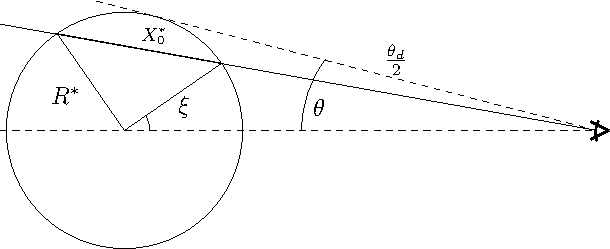
\includegraphics[width=0.7\textwidth]{C:/Users/henri/OneDrive/Documents/NTNU/Semester 10/Masteroppgave/Plots/Radiative_transfer_SSA.pdf}
    \caption{Schematic view of the radiative transfer in a spherical ball of plasma. Image inspired by image from \cite{Hirotani_2005}}
    \label{fig:Radiative_transfer}
\end{figure}

\subsection{Deviation from SSA and Equipartition}
If one calculates the magnetic field using both SSA and Equipartition one expects to not get the exact same results, but given a big discrepancy one cannot assume all the fault lies in only the measurements. In \cite{10.1093/mnras/stt2217}, who used SSA and equipartition calculations for a small sample of CSOs, they also found a discrepancy between the two methods. The SSA had a significantly higher value for the magnetic field. This they argue can, and the weight is on can here, be induced by a free-free absorption effect in the source. Free-free absorption is the absorption of radiation by an electron who is in proximity to an ion. The absorption is a result of the electron being accelerated by the ion and the radiation emitted by the electron is absorbed by the ion. The effect of free-free absorption would shift the spectral peak in SSA to a higher frequency and thus give a higher magnetic field strength in our calculations. This would be a good indicator that the source is harboring ions, which one needs for UHECRs acceleration.

\section{Time-scales analysis}
\label{sec:time_scales}

In order to probe what type of sources could be responsible for the observed UHECRs and neutrinos one can use the relevant time-scales as a measure. The timescales of a source will act as an indicator of the dominant processes in the source and give us an upper boundary for what we could expect of escaping particles. The dominant timescales of a source will be source specific, so further on we will be looking at the timescales of a typical compact AGN. The relevant timescales are the acceleration timescale, the synchrotron cooling timescale, the dynamical timescale, and the photo-pion cooling timescale.

\textbf{Acceleration timescale:}
One starts by determining the acceleration timescale of a proton undergoing first-order Fermi acceleration, the acceleration mechanisms explained in section \ref{sec:acceleration_mechanisms}. The acceleration timescale is given by the equation
\begin{equation}
    t_{acc} =  \frac{\eta \epsilon}{Z e B c}
\end{equation}
Where $\eta$ is the efficiency of the acceleration process with the most efficient acceleration harboring the value $\eta \approx (1-10)$, $\epsilon$ is the energy of the particle, $Z$ is the charge of the particle, $e$ is the elementary charge, $B$ is the magnetic field strength and $c$ is the speed of light. 
Usually the value of $\eta$ is taken to be 1, which is the most efficient acceleration process.

\textbf{Size estimation/ dynamical timescale:}
\label{sec:size_estimation}

The dynamical timescale is a limit on the source's size and can be estimated several ways. The source's size is important since in order to accelerate particles the source must also be able to contain particles. If one does not have good measurements on the source size, but has good fluence measurements of an attributing light curve, one can estimate the size of the source via the variability. From the variability timescale $t_{var}$ one can estimate the size of the source as

\begin{equation}
    R = \frac{c \Gamma t_{var}}{1+z}
\end{equation}

Another way of estimating the source's size is through telescope measurements. For radio sources, one can achieve sufficient accuracy in measurements to estimate the size of the source. If one has the full width at half maximum of an emitting sphere, one can relate this to the total angular size of a spherical source according to \cite{1983ApJ...264..296M} as $\theta = \theta_{\text{FWHM}} 1.8$. If one then knows the distance to the source one can get the physical/linear size of the source as

\begin{equation}
    D_{\text{size}} = \left(\theta_{\text{FWHM}}1.8 \right) \cdot D_A(z)
\end{equation}

Where $D_A(z)$ is the angular diameter distance to the source at its redshift $z$.

A third method of estimating the size of specifically the radius of our radio lobes is outlined in \cite{W_jtowicz_2020}. They use a relation between the total linear size of an object and the estimated relations between the semi-major axis and the semi-minor axis. The argument is that some AGN which are important for this report have relatively large aspect ratios between their axes, with an estimation equaling $b/a \approx 0.25$. From this, they introduce the effective radius of the radio lobes via

\begin{equation}
    R_{\text{lobe}} = \sqrt[3]{ab^2\frac{3}{4}} \approx 0.18 \times LS = 0.18 \times 2 \times a 
\end{equation}


\textbf{Cooling timescales:}

In the source of AGN there will be an environment of magnetic fields and photon fields that will interact with the particles. An important timescale to consider given this environment is often the synchrotron cooling timescale. This is the timescale for a particle to lose energy due to synchrotron radiation. One will have both synchrotron losses for proton and for electrons, but since one is concerned about UHECRs one will focus on protons. The synchrotron cooling timescale for protons is given by the equation

\begin{equation}
    t_{sync} = \frac{6\pi m_p^4 c^3}{\sigma_T m_e^2 B^2 E}.
\end{equation}

Here, $m_p$ is the proton mass, $m_e$ is the electron mass, $\sigma_T$ is the Thomson cross-section, $B$ is the magnetic field strength, $E$ is the energy of the particle, and $c$ is the speed of light.

The last timescale used in this analysis is the pion production timescale. Due to the photon fields a proton will inhabit while accelerating, one needs to consider the pion production timescale. This is the timescale for a proton to interact with a photon and produce a pion. The equation is given by
\begin{equation}
    t_{p\gamma}^{-1}(\varepsilon_p) = \frac{c}{2\gamma_p^2} \int_{\varepsilon_{th}}^{\infty} d\varepsilon \sigma_{pr}(\varepsilon) k_p(\varepsilon) \int_{\varepsilon/2\gamma_p}^{\infty} d\varepsilon' \varepsilon'^{-2} \frac{dn}{d\varepsilon'}
\end{equation}
where $\varepsilon_p$ is the energy of the proton, $\gamma_p$ is the Lorentz factor of the proton, $\varepsilon_{th}$ is the threshold energy for the interaction, $\sigma_{pr}$ is the cross-section for the interaction, $k_p$ is the photon field, and $dn/d\varepsilon$ is the differential photon density.

In our analysis one will follow \cite{BHradiation} to set up the pion resonance timescale. $\sigma_{pr}$, or the cross-section for the interaction is given by a two-step function, and is given as

\begin{equation}
    \sigma(E) = 
    \begin{cases} 
    340 \mu b, \text{cm}^{-2} & \text{if } 390 m_e c^2 < E < 980 m_e c^2 \\
    120 \mu b \, \text{cm}^{-2} & \text{if } E > 980 m_e c^2 
    \end{cases}
\end{equation}

Additionally, the inelasticity of the interaction, or how much energy is lost per interaction, is given as

\begin{equation}
    K(E) = 
    \begin{cases} 
    0.2 & \text{if } 390 m_e c^2 < E < 980 m_e c^2 \\
    0.6 & \text{if } E > 980 m_e c^2 \\
    \end{cases}
\end{equation}

%\begin{figure}
%    \centering
%    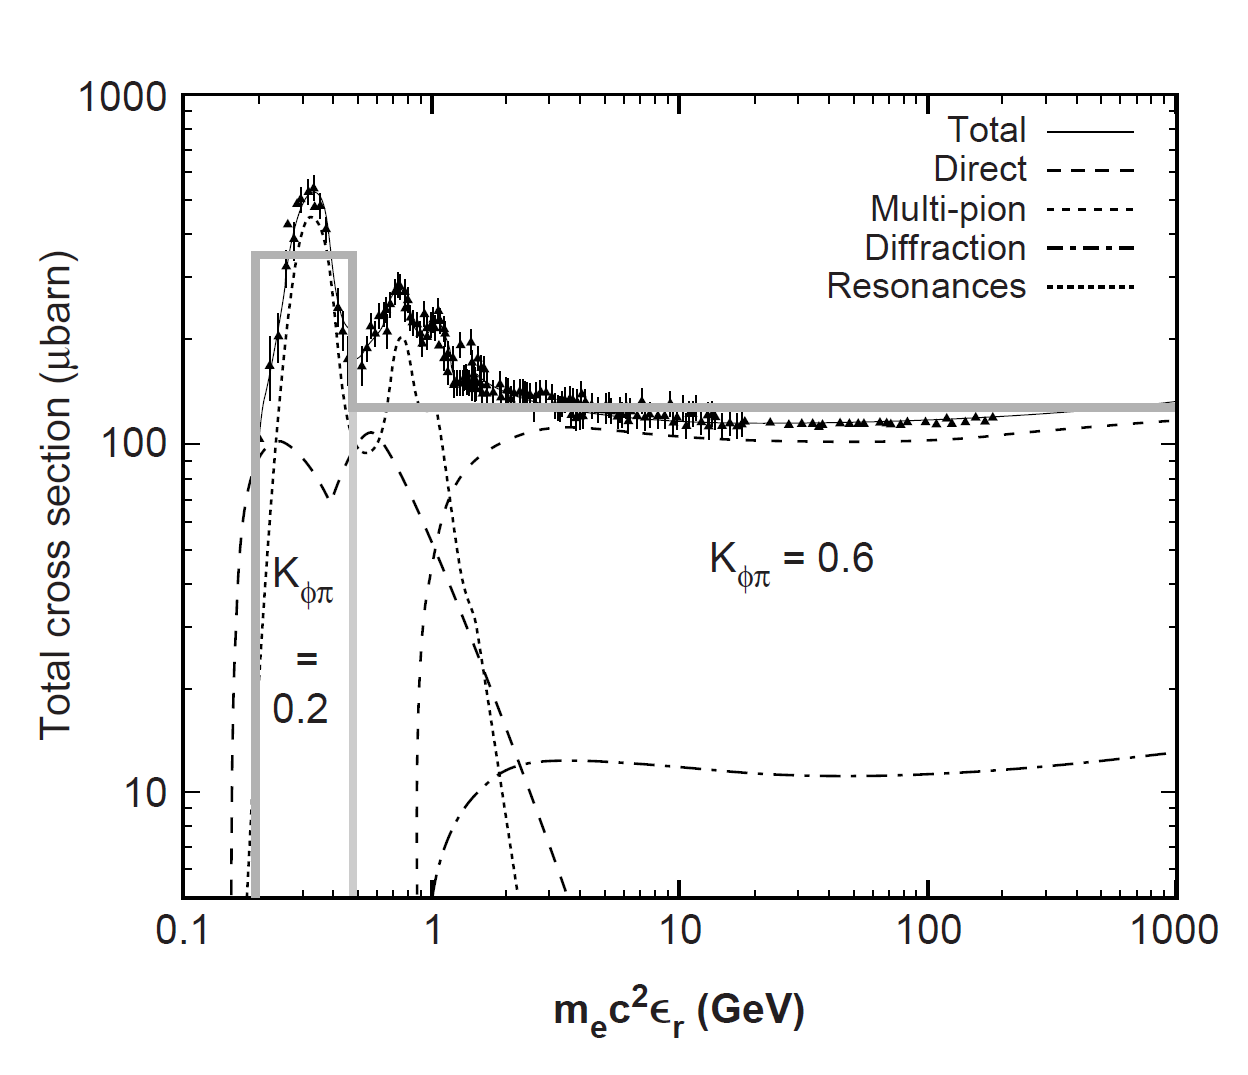
\includegraphics[width=0.5\textwidth]{C:/Users/henri/OneDrive/Documents/NTNU/Semester 10/Masteroppgave/Plots/Dermer_pion_res.png}
%    \caption{Pion resonance cross-section, and the inelasticity of the interaction. Image taken from \cite{BHradiation}}
%    \label{fig:pion_res}
%\end{figure}

%A schematic view of the pion resonance cross-section and the inelasticity of the interaction is shown in Figure \ref{fig:pion_res}. 

The last important parameter in the pion production timescale is the photon field, and one will be using a photon field as described in section \ref{sec:photon_fields}. The specific photon fields will be determined by what source one is looking at and will be clarified in due time.

\newpage

\chapter{Compact symmetric objects}
\section{Compact symmetric objects}
\begin{enumerate}
    \item Introduction to CSOs
    \item What is a CSO
    \item more on the structure of CSOs
    \item The different types of CSOs
    \item The prevalence of CSOs 
    \item CSO as candidates for UHECRs and neutrinos
    \begin{enumerate}
        
       
        \item Hillas criterion, Flux of X-ray compared to diffuse flux of UHECRs and neutrinos 
        \item Kinetic jet power
        \item Timescale analysis
    \end{enumerate}
\end{enumerate}

\subsection*{Introduction to CSOs}

Compact Symmetric Objects have seen a revival the last year with the publication of \cite{kiehlmann2023compact} and \cite{readhead2023compact}. The original discovery of CSOs was in the 1980s when according to \cite{kiehlmann2023compact} Phillips and Mutel discovered a class of compact extragalactic radio galaxies with symmetric radio structures, or harbouring a compact double radio source which was not the core. This was a break from the usual suspects of most jetted-AGN which usually shows great effect of relativistic beaming. Following the discovery of the compact double source more discoveries of CSOs were made, and in the 90s the origial motivation for the CSO classification was given. According to \cite{kiehlmann2023compact} this classification lead to the misidentification of AGNs as CSO and rendering the classification less useful. In the last year the classification has been revisited and a updated list of criteria for CSOs has been given. This paper will follow the new classification of CSOs and use the updated list of CSOs from \cite{kiehlmann2023compact}.

The classification of CSO can be summeraized in four points taken from \cite{kiehlmann2023compact}. 

\begin{enumerate}
    \item Size requirement: No projected radio structure larger than 1kpc. This has an exception to relic regions which might be signs of previous activity. 
    \item Symmetry requirement: Evidence of emission on both sides of the core. 
    \item Variability requirement: The source should not exhibit fractional variablility of $20\%$ or more per year 
    \item relativistic requirement: The source components should not show signs of superluminal motion greater than $v_{app} = 2.5c$ 
\end{enumerate}

The size requirement is a key feature of CSOs since it is what makes them compact, and has previously been used to classify CSOs. Structures larger than 1kpc are often refered to as medium symmetric objects(MSO) and structures larger than that as Large symmetric object(LSO). The reason for these limits is that is approximatley corresponds to the boundary between regions dominated by tge black hold and the region dominated by the galaxy, and region dominated by the galaxy and the region dominated by the extra galactic environment. this then places CSOs in the region where the black hole is the dominant force. In additon to this size requirement, \cite{kiehlmann2023compact} added a caveat. Some CSOs show relic regions which are signs of previous activity. These regions can extend to larger distances than the 1kpc limit, but should not be the dominant feature of the source.

The symmetry requirement also has some caveat. CSOs are object that show any symmetric emission, but not necessarly of similar magnitude. In addition, the placement of the core is either inferred from a compact flat specturm component, or from the symmetry of the radio lobes. In figure \ref{fig:CSO_J0741} one can see how one would determine the core placement from both the flat spectrum component and the symmetry of the radio lobes.

\begin{figure}
    \centering
    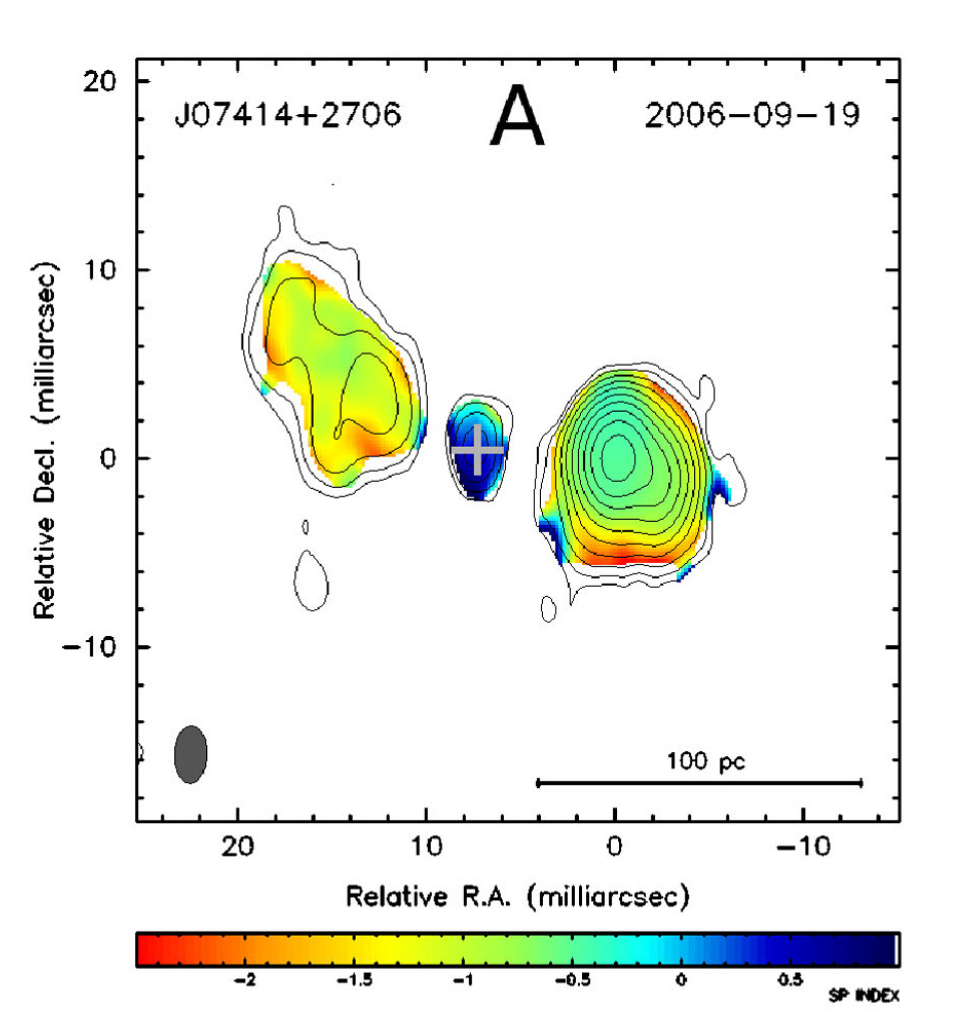
\includegraphics[width=.5\textwidth]{C:/Users/henri/OneDrive/Documents/NTNU/Semester 10/Masteroppgave/Plots/J0741+2706.png}
    \caption{The radio structure of CSO J0741+2706. The core is determined from the flat spectrum component and the symmetry of the radio lobes. Image taken from \cite{Tremblay_2016}}
    \label{fig:CSO_J0741}
\end{figure}

The last two criteria are the newest addition made by \cite{kiehlmann2023compact} and is the best way of separating CSOs from other jetted AGNs. The low variability and lack of relativisitic beaming has always been a key feature of CSOs, but since they were not included in the original classification there have been misidentification. An example quoted in \cite{kiehlmann2023compact} is the source PKS 1543+005 which shows strong variability and additionally the jet is projected on both sides of the core, giving the illusion of a compact double. With these new criteria one can be more certain that the sources in the catalogue are similar enough in nature to be able to make more general statements about them.





%\subsubsection*{Total energy density}
%The total energy density of the photon fields as a function of distance is then seen in figure \ref{fig:photon_fields}. Here one can see that the energy density of the photon fields is constant until the observer is outside the size of the respective regions. From the image it is clear that the biggest contributor to the total energy density becomes the IR torus, but all the regions contribute significantly to the total energy density.

%\subsubsection*{Spectral energy density}
%The spectral energy density of the different regions is of more interest since this is what will determine the effect of pion decay on protons accelerate in the jet or in the lobes. To create the 
%SED one has estimated the dynamical scale of our system and used the total photon densities to scale the SED accordingly. The resulting SED is seen in figure \ref{fig:SED_sep}. The SED are determined also on a number of 
%parameters, all which have taken from the literature. They are seen in table \ref{tab:SED_params}.

%The choice of variables comes from three sources. \cite{bronzini2024investigating} and \cite{kiehlmann2023compact} which both gives the disk luminosity of CSOs sources, and which we set to $10^{43} erg/s$. \cite{Ghisellini_2009} gives the rest of parameters that relate the different regions to the disk luminosity. The biggest caveat here is that these parameters are not specific to CSOs, but to Blazars in which they are based. For the purposes of this analysis one assumes that the parameters are the same for CSOs as for Blazars, and that one would not expect any significant difference. 

\begin{table}
    \centering
    \begin{tabular}{|c|c|}
        \hline
        Parameter & Value \\
        \hline
        $L_{d}$ & $10^{43}$ erg/s \\
        $GM$ & $G 10^{8} M_{\odot}$ \\
        $RS$ & $\frac{2GM}{c^2}$ \\
        $\eta$ & 0.1 \\
        $f_{X}$ & 0.3 \\
        $R_{X}$ & 30$ RS $\\
        $\beta$ & 0.4 $c$\\
        $f_{\text{BLR}}$ & 0.1 \\
        $R_{\text{BLR}}$ & $10^{17} \sqrt{L_{d}/10^{45}}$ cm \\
        $f_{\text{IR}}$ & 0.5 \\
        $R_{\text{IR}}$ & $2.5 10^{18}\sqrt{L_{d}/10^{45}}$ cm \\
        $\Gamma$ & 1.1 \\
        \hline
    \end{tabular}
    \caption{Parameters used to determine the SED of the different regions.}
    \label{tab:SED_params}
\end{table}
\begin{figure}
    \centering
    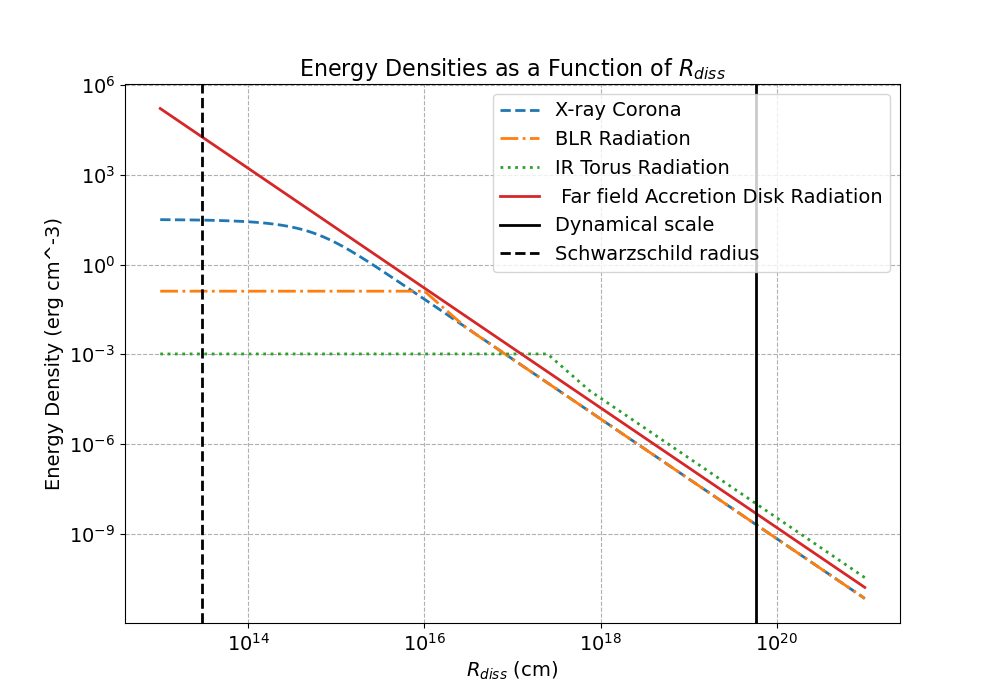
\includegraphics[width=.5\textwidth]{C:/Users/henri/OneDrive/Documents/NTNU/Semester 10/Masteroppgave/Plots/Energy_densities.png}
    \caption{The total energy density of the photon fields as a function radius from central engine.}
    \label{fig:photon_fields}
\end{figure}


\begin{figure}
    \centering
    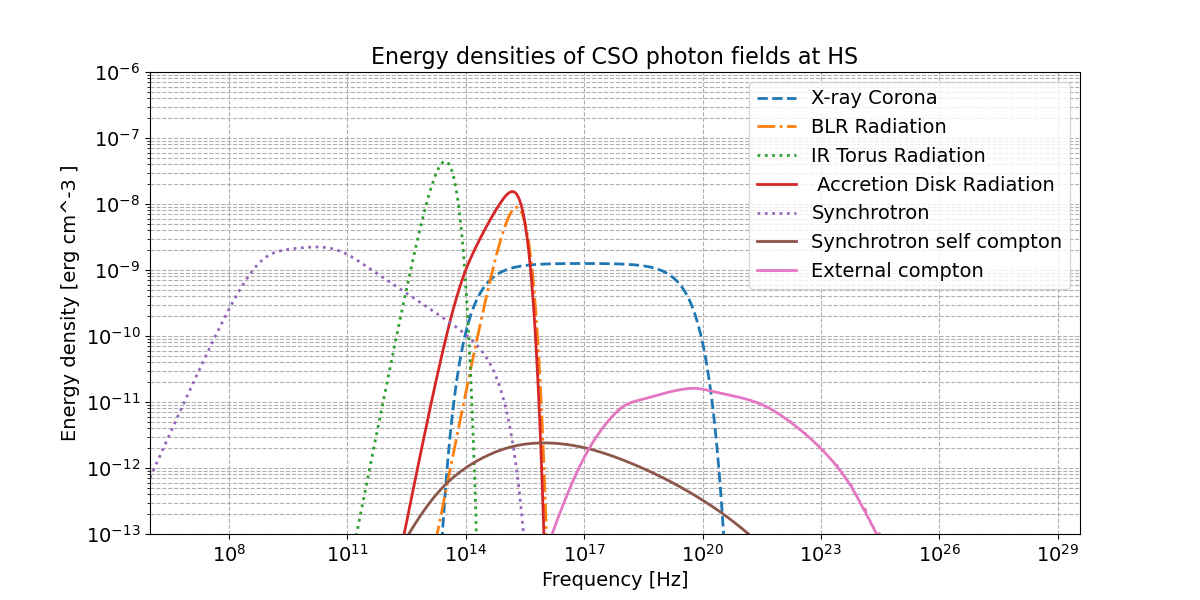
\includegraphics[width=.5\textwidth]{C:/Users/henri/OneDrive/Documents/NTNU/Semester 10/Masteroppgave/Plots/SEDs_sep.png}
    \caption{The spectral energy density at distance R}
    \label{fig:SED_sep}
\end{figure}

\begin{figure}
    \centering
    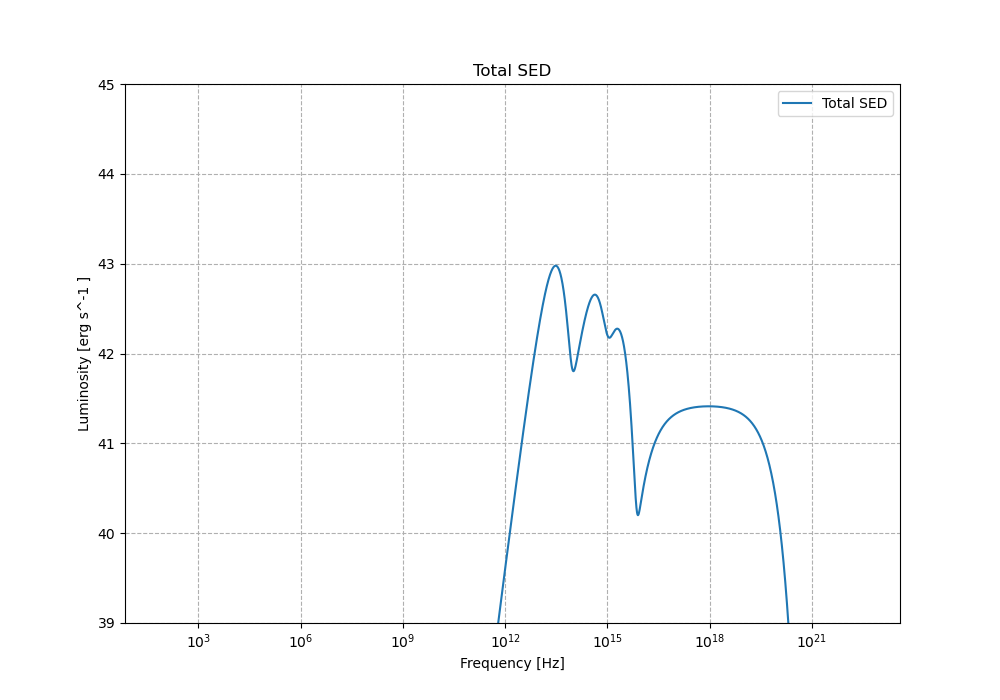
\includegraphics[width=.5\textwidth]{C:/Users/henri/OneDrive/Documents/NTNU/Semester 10/Masteroppgave/Plots/SED.png}
    \caption{Luminosity of the different components of the CSO that are close by the central engine. Missing synchrotron and IC part which is most prominent }
    \label{fig:Lum_SED}
\end{figure}

\subsection{Sub Classification of CSO}
Moving further along the classification of CSOs one now realises that there are two types of CSOs. CSO 2 and CSO 1. In CSO 2 sources one consider it edge brightened where there is significant luminosity in the radio lobes compared to the core. In CSO 1 sources one consider it edge dimmed where the luminosity of the radio lobes are significantly lower than that of the core. The origin of the two types of CSOs are thought to be the same, where CSO 1s represent failed CSO 2s. One will get back to the origin later in the report.

The fact of the matter is that also the CSO 2 class can further be subdivided. This extra subdivsion into CSO 2.0, 2.1, and 2.2 is on the basis of its morphology. In the number of Compact symmetric objects which succeed into becoming CSO 2s will go through different phases all with different characteristics. In figure \ref{fig:CSO_2_morphology} one can visualise the different phases of CSO 2 sources. The phases can analogously be compared to the different phases of shock evolution in supernovae.

\begin{figure}
    \centering
    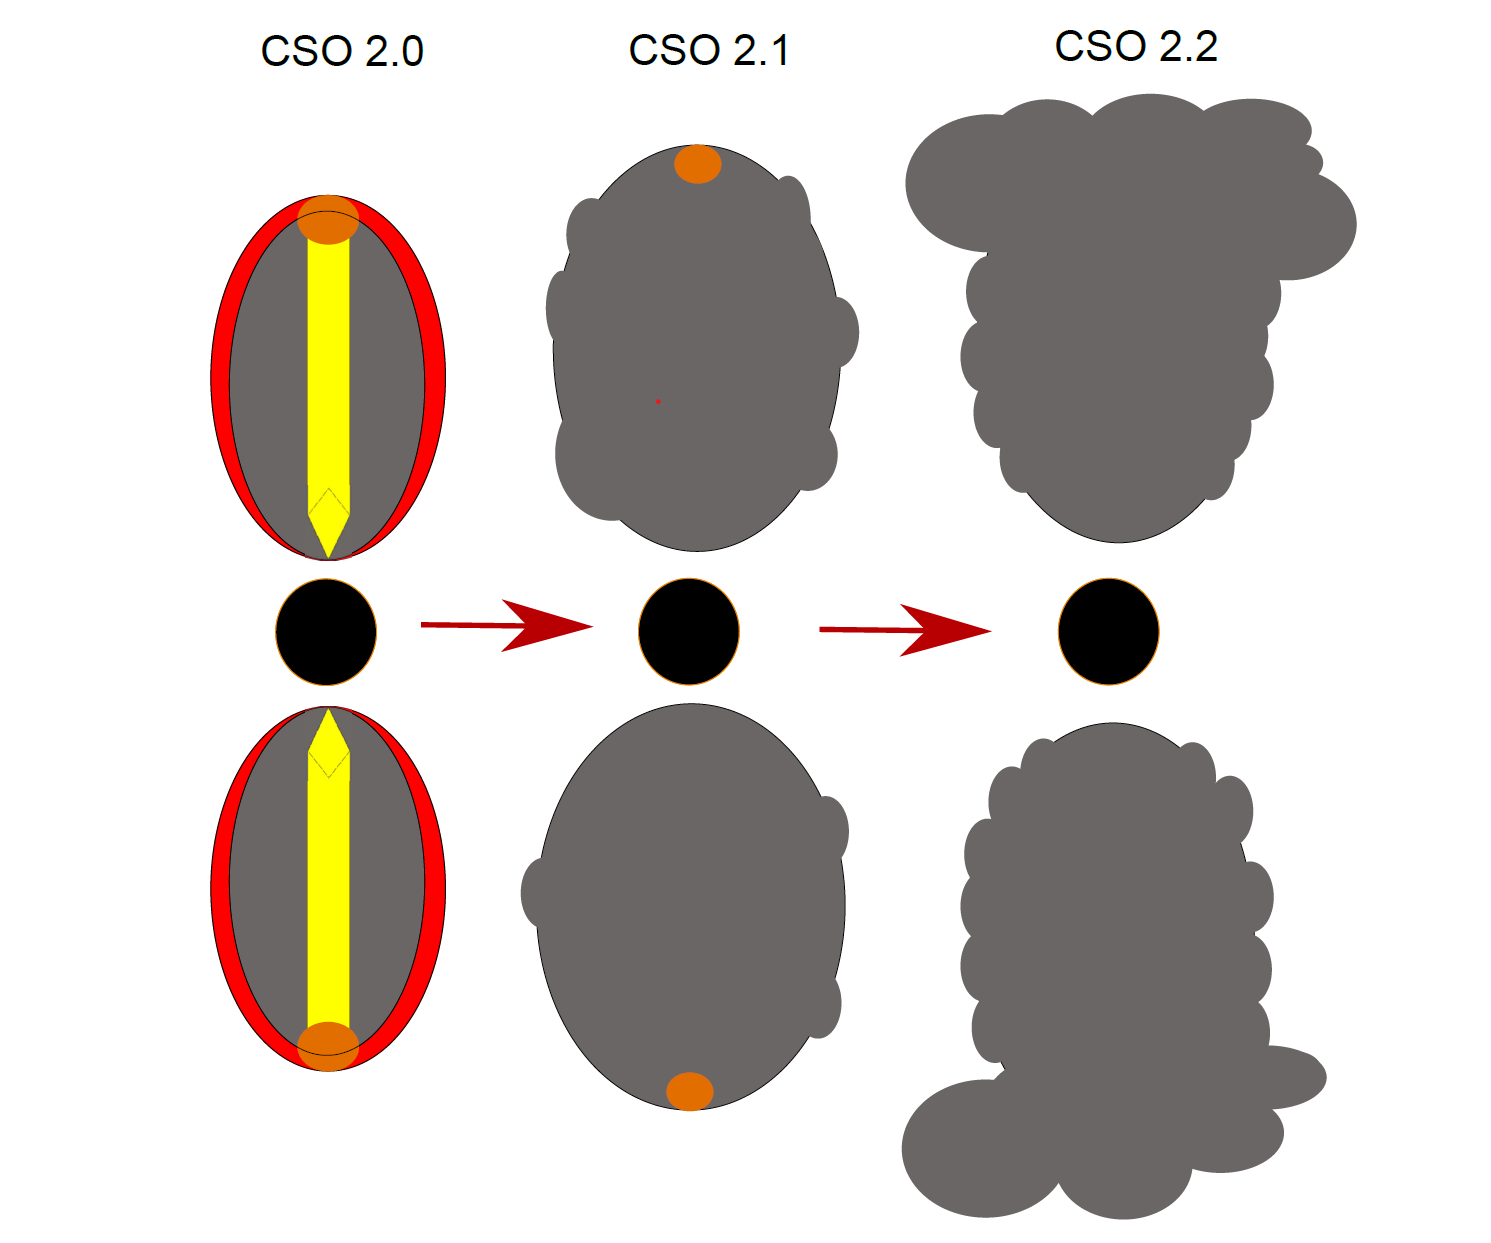
\includegraphics[width=.8\textwidth]{C:/Users/henri/OneDrive/Documents/NTNU/Semester 10/Masteroppgave/Plots/CSO_morphology.png}
    \caption{The different phases of CSO 2 sources. Image taken from \cite{sullivan2024smallscale}}
    \label{fig:CSO_2_morphology}
\end{figure}

\textbf{CSO 2.0}: According to \cite{sullivan2024smallscale} the CSO 2.0 phase evolves analogously to FRII radio galaxies. The edge-brightened lobes which contain prominent hot spots are similar to typical features of a relativitic jet pushing into the ambient medium. As \cite{sullivan2024smallscale} points out, classical jet models entail the jet collides with the ambient medium and forms two shock front, the forward shock and the reverse shock. From shock models the jet power $L_j$ is what determines the velocity of the forward shock, and in \cite{sullivan2024smallscale} the shock model used gives values similar to observation of CSO 2.0 lobe velocity($v_c = 0.2c$) and mach number of approximately $200$.

\textbf{CSO 2.1}: The mid life or CSO 2.1 is the transition of relativistic jet propagation into the sonic of subsonic regime. The category is often hard to define and is often contaminated by a  mix of CSO 2.0 and CSO 2.2. Nevertheless, it remains a separate category since there is still power in the hotspots and the lobes continue to expand but decelerate. 

\textbf{CSO 2.2}: The late life of CSOs or CSO 2.2 is the phase where the jet has decelerated to transonic speeds and the lobes are no longer expanding vertically as a result of jet pressure. The lobes are still expanding due to convectively rising turbulent plumes. When the plumes and the ambient densities are equal the lobes will stop expanding vertically and start expanding horizontally. \cite{sullivan2024smallscale} compares it to the characteristic mushroom cloud of volcanic which in this author's opinion paints a very nice image. 

This separation of CSOs will become important since certain enviroments are more favourable for the production of UHECRs and neutrinos. The most promising candidate are CSO 2.0 sources since they have the highest jet power and the highest velocity of the lobes. 

\subsection{Origin of CSOs/Fueling}
According to \cite{readhead2023compact} a possible method of fueling these objects is through tidal disruption events. Due to the short lifetime of these objects continued discrete fueling events become a good candidate for the ignition of the jets. Energetically one would assume that one needs a massive star to be able to fuel the CSO $2$ jets, but it is argued in \cite{sullivan2024smallscale} that this might not be the only solution. They argue that smaller mass stars which encounter the black hole could have sufficient magnetic flux to ignite the extraction of the black holes angular momentum. The method proposed in \cite{Blandford_1977} relate the extraction of black hole angular momentum  to the jet power via 

\begin{equation}
    L_j = \frac{1}{6\pi c} \Omega_{BH}^2 \Phi_{BH}^2
\end{equation}

After the TDE one expects the magnetic flux to disperse around the BH as $\Phi_{BH} \approx \Phi_{\star} \left(\frac{R_{H}}{R_{p}}\right)^2$ where $R_{H}$ is the black hole horizon and $R_{p}$ is the pericenter radius of the stellar encounter. In addition, the magnetic field could be amplified via strong dipolar dynamo action or magneto-rotational instability. The magnetic field could be strong enough to match the jet powers one observes in CSOs today even though the original stellar mass was low.The caveat here is that amplification of the magnetic field is required to reach sufficient levels.  


%It is argued in \cite{sullivan2024smallscale} that the introduction of external magnetic flux into an already existing seed field, created by possibly the accretion disk will lead to amplification of the magnetic field through extration of black hole angular momentum, \cite{Blandford_1977}. 

Along with the energetics one can put simple tests on this hypothosis by looking at the fallback time of debris onto a central black hole. This is also done in \cite{sullivan2024smallscale} which quote the fallback time as 

\begin{equation}
    t_f = 0.5 \text{yr}\left(\frac{M_{\rm BH}}{10^8 M_{\odot}}\right)^{1/2}\left(\frac{M_\star}{M_{\odot}}\right)^{-1}\left(\frac{R_\star}{R_{\odot}}\right)^{3/2}
\end{equation}

For the TDE hypothesis to be correct one would expect the fallback time to be of the order of the lifetime of the CSO 2.0, which is $t_f \approx 1000$ years. From the equation above red giants become a good candidate as they have a large radius and a low mass, and with a SMBH of $10^8 M_{\odot}$ the fallback time is of the order of $1000$ years.

Small sizes and finite lifetime are good indicators for transient events, and this is quoted in \cite{sullivan2024smallscale}


%From the papers of \cite{kiehlmann2023compact} to \cite{readhead2023compact}, and from \cite{sullivan2024smallscale} there is a clear quite new classification of CSOs. The classification is based on firstly CSOs being edge brightened or edge dimmed. Edge brightened sources which will onwards be refered as CSO 2s are bright in radio in their lobes, and CSO 1s or edge dimmed are thought to be CSOs that have stalled. 

%The big picture on CSOs is that they are a group of very short-lived sources that are ignited by transient events. Saying if the ignition of their jets are due to transient event such as tidal disruption event are covered in \cite{sullivan2024smallscale} and for the purposes of this study not necessary to discuss, but start a very interesting conversation. CSOs are then symmetric with the expansion of their jets into the interstellar medium visible from radio telescope. The symmetry of the jets is a key feature of CSOs and makes them unique in the sense of jetted-AGN since they have little to no features of relativistic beaming.   


\subsection{Catalouge of Bona fide CSO}
With the new criterias for CSOs \cite{kiehlmann2023compact} begun compiling a bone fide list of Compact symmetric objects. This new catalogue will serve as the testing grounds for their ability to produce UHECRs and neutrinos. The catalogue is a list of 79 sources which are somewhat split between the four different subclasses as seen in table \ref{tab:CSO_class} where only the CSO with a spectroscopic redshift have been given a class. The full source catalogue is listed in table \ref{tab:CSO_sources}.
%In order to study these sources there will always be a need for observational data. This fact combined with the fact that CSOs are a somewhat new class of AGN mean that there are no large catalogues of pure CSOs, and that many other catalogues misnomer sources as CSOs. This chapter will rely heavilly on \cite{kiehlmann2023compact} in which this is discussed and where they define a bona fide catalogue of 79 CSOs. The catalogue will allow us as it has in this paper to say more concrete information about the sources we are studying.
\begin{table}[H]
    \centering
    \caption{Catalouge of bona fide CSOs. Data taken from \cite{kiehlmann2023compact}}
    \label{tab:CSO_sources}
    \begin{tabular}{@{}ccccccccc@{}}
        \toprule
        ID & R.A. & Dec. & z & Ang\_size & Lin\_size & $\nu_t$ & $S_\nu$ & Class \\ \midrule
        J0000+4054 & 00:00:53.08 & +40:54:01.81 & nan & 124.0 & nan & 0.323 & 2.06 & nan \\
        J0003+4807 & 00:03:46.04 & +48:07:04.14 & nan & 16.2 & 0.139 & 2.123 & 0.348 & nan \\
        J0029+3456 & 00:29:14.24 & +34:56:32.25 & 0.517 & 29.1 & 0.180 & 0.8 & 2.0 & 2.1 \\
        J0111+3906 & 01:11:37.32 & +39:06:28.10 & 0.66847 & 8.0 & 0.056 & 4.0 & 1.33 & 2.0 \\
        J0119+3210 & 01:19:35.00 & +32:10:50.06 & 0.0602 & 100.0 & 0.115 & 0.4 & 4.0 & 2.2 \\
        J0131+5545 & 01:31:13.82 & +55:45:12.98 & 0.003649 & 23.0 & 0.016 & 0.657 & 0.31 & 2.2 \\
        J0132+5620 & 01:32:20.45 & +56:20:40.37 & nan & 12.2 & 0.104 & 3.42 & 0.6 & nan \\
        J0150+4017 & 01:50:19.61 & +40:17:30.02 & nan & 103.0 & 0.882 & 0.4 & 2.0 & nan \\
        J0204+0903 & 02:04:34.76 & +09:03:49.26 & nan & 33.0 & 0.282 & 1.3 & 2.0 & nan \\
        J0237+4342 & 02:37:01.21 & +43:42:04.18 & nan & 120.0 & nan & 0.3 & 0.868 & nan \\
        J0402+8241 & 04:02:12.68 & +82:41:35.13 & nan & 72.0 & 0.616 & 0.4 & 0.4 & nan \\
        J0405+3803 & 04:05:49.26 & +38:03:32.24 & 0.05505 & 42.0 & 0.044 & 0.07 & 5.5 & 2.0 \\
        J0425-1612 & 04:25:53.57 & -16:12:40.23 & nan & 99.8 & 0.854 & 0.363 & 1.449 & nan \\
        J0427+4133 & 04:27:46.05 & +41:33:01.10 & nan & 7.0 & 0.060 & 3.3 & 0.74 & nan \\
        J0440+6157 & 04:40:46.90 & +61:57:58.57 & nan & 30.0 & 0.257 & 1.7 & 0.24 & nan \\
        J0706+4647 & 07:06:48.07 & +46:47:56.45 & nan & 63.0 & 0.539 & 0.777 & 1.81 & nan \\
        J0713+4349 & 07:13:38.16 & +43:49:17.21 & 0.518 & 35.0 & 0.217 & 1.9 & 2.09 & 2.0 \\
        J0735-1735 & 07:35:45.81 & -17:35:48.50 & nan & 28.8 & 0.246 & 1.4 & 3.0 & nan \\
        J0741+2706 & 07:41:25.73 & +27:06:45.42 & 0.772139 & 26.0 & 0.193 & 1.0 & 1.05 & 2.0 \\
        J0754+5324 & 07:54:15.22 & +53:24:56.45 & nan & 26.0 & 0.223 & 1.24 & 0.634 & nan \\
        J0825+3919 & 08:25:23.68 & +39:19:45.76 & 1.21 & 70.7 & 0.591 & 0.517 & 1.77 & 2.1 \\
        J0832+1832 & 08:32:16.04 & +18:32:12.12 & 0.154 & 30.7 & 0.081 & 1.5 & 1.2 & 1 \\
        J0855+5751 & 08:55:21.36 & +57:51:44.09 & 0.025998 & 75.0 & 0.039 & 0.3 & 1.5 & 2.1 \\
        J0906+4124 & 09:06:52.80 & +41:24:30.00 & 0.0273577 & 11.1 & 0.006 & 1.5 & 0.06 & 1 \\
        J0909+1928 & 09:09:37.44 & +19:28:08.30 & 0.027843 & 14.7 & 0.008 & 6.0 & 0.12 & 1 \\
        J0943+1702 & 09:43:17.23 & +17:02:18.97 & 1.601115 & 20.4 & 0.175 & 4.0 & 0.4 & 2.0 \\
        J1011+4204 & 10:11:54.18 & +42:04:33.38 & nan & 115.0 & 0.984 & 0.424 & 1.16 & nan \\
        J1025+1022 & 10:25:44.20 & +10:22:30.00 & 0.045805 & 19.8 & 0.018 & 1.0 & 0.09 & 1 \\
        J1035+5628 & 10:35:07.04 & +56:28:46.79 & 0.46 & 38.0 & 0.221 & 1.3 & 1.87 & 2.0 \\
        J1042+2949 & 10:42:36.51 & +29:49:45.15 & nan & 45.0 & 0.385 & 0.7 & 1.0 & nan \\
        J1111+1955 & 11:11:20.07 & +19:55:36.01 & 0.299 & 15.5 & 0.068 & 1.305 & 1.1 & 2.0 \\
        J1120+1420 & 11:20:27.81 & +14:20:54.97 & 0.362 & 101.0 & 0.507 & 0.5 & 3.89 & 2.0 \\
        J1135+4258 & 11:35:55.99 & +42:58:44.65 & nan & 29.0 & 0.248 & 1.0 & 1.45 & nan \\
        J1148+5924 & 11:48:50.36 & +59:24:56.36 & 0.01075 & 54.8 & 0.012 & 6.149 & 0.573 & 1 \\
        J1158+2450 & 11:58:25.79 & +24:50:18.00 & 0.203 & 46.0 & 0.152 & 2.0 & 1.25 & 2.2 \\
        J1159+5820 & 11:59:48.77 & +58:20:20.31 & 1.27997 & 70.2 & 0.591 & 0.6 & 1.9 & 2.0 \\
        J1204+5202 & 12:04:18.61 & +52:02:17.62 & nan & 54.0 & 0.462 & 0.7 & 1.4 & nan \\

        \bottomrule
    \end{tabular}
\end{table}

\begin{table}
    \centering
    \begin{tabular}{@{}ccccccccc@{}}
        \toprule
        ID & R.A. & Dec. & z & Ang\_size & Lin\_size & $\nu_t$ & $S_\nu$ & Class \\ \midrule
        J1205+2031 & 12:05:51.50 & +20:31:19.00 & 0.02378857 & 22.0 & 0.010 & 1 & 0.14 & 2.1 \\
        J1220+2916 & 12:20:06.82 & +29:16:50.72 & 0.002 & 46.8 & 0.002 & 0.074 & 0.65 & 1 \\
        J1227+3635 & 12:27:58.72 & +36:35:11.82 & 1.975 & 58.8 & 0.499 & 1.2 & 2.14 & 2.0 \\
        J1234+4753 & 12:34:13.33 & +47:53:51.24 & 0.373082 & 27.4 & 0.140 & 1.4 & 0.36 & 2.1 \\
        J1244+4048 & 12:44:49.19 & +40:48:06.15 & 0.813586 & 70.0 & 0.529 & 0.405 & 2.03 & 2.2 \\
        J1247+6723 & 12:47:33.33 & +67:23:16.45 & 0.107219 & 5.0 & 0.010 & 1.16 & 0.36 & 2.0 \\
        J1254+1856 & 12:54:33.27 & +18:56:01.93 & 0.1145 & 4.14 & 0.008 & 6.0 & 0.13 & 1 \\
        J1311+1658 & 13:11:23.82 & +16:58:44.22 & 0.081408 & 27.0 & 0.041 & 0.447 & 0.824 & 1 \\
        J1313+5458 & 13:13:37.85 & +54:58:23.91 & 0.613 & 57.0 & 0.384 & 0.555 & 1.65 & 2.2 \\
        J1326+3154 & 13:26:16.51 & +31:54:09.52 & 0.36801 & 68.0 & 0.345 & 0.5 & 7.03 & 2.2 \\
        J1335+5844 & 13:35:25.93 & +58:44:00.29 & nan & 12.9 & 0.110 & 4.9 & 0.9 & nan \\
        J1347+1217 & 13:47:33.36 & +12:17:24.24 & 0.121 & 100.0 & 0.215 & 0.4 & 8.86 & 2.2 \\
        J1400+6210 & 14:00:28.65 & +62:10:38.59 & 0.431 & 67.6 & 0.378 & 0.5 & 6.56 & 2.2 \\
        J1407+2827 & 14:07:00.40 & +28:27:14.69 & 0.077 & 11.0 & 0.016 & 4.9 & 3.0 & 2.1 \\
        J1413+1509 & 14:13:41.66 & +15:09:39.51 & nan & 15.0 & 0.128 & 2.5 & 0.47 & nan \\
        J1414+4554 & 14:14:14.85 & +45:54:48.73 & 0.186 & 30.5 & 0.094 & 0.693 & 0.396 & 2.1 \\
        J1416+3444 & 14:16:04.18 & +34:44:24 & nan & 81.0 & 0.693 & 0.7 & 2.1 & nan \\
        J1434+4236 & 14:34:27.86 & +42:36:20.06 & 0.452 & 68.3 & 0.393 & 0.074 & 1.67 & 2.2 \\
        J1440+6108 & 14:40:17.87 & +61:08:42.88 & 0.445365 & 30.0 & 0.171 & 0.4 & 0.48 & 2.1 \\
        J1443+4044 & 14:42:59.32 & +40:44:28.94 & nan & 123.4 & nan & 0.292 & 1.55 & nan \\
        J1508+3423 & 15:08:05.70 & +34:23:23.00 & 0.045565 & 280.0 & 0.247 & 0.23 & 0.25 & 2.1 \\
        J1511+0518 & 15:11:41.27 & +05:18:09.26 & 0.084 & 10.6 & 0.017 & 0.4 & 0.48 & 2.0 \\
        J1559+5924 & 15:59:01.70 & +59:24:21.84 & 0.0602 & 11.0 & 0.013 & 0.15 & 0.23 & 1 \\
        J1602+5243 & 16:02:46.38 & +52:43:58.40 & 0.105689 & 250.0 & 0.478 & 0.15 & 1.48 & 1 \\
        J1609+2641 & 16:09:13.32 & +26:41:29.04 & 0.473 & 61.3 & 0.362 & 1.1 & 5.44 & 2.1 \\
        J1645+2536 & 16:44:59.07 & +25:36:30.64 & 0.588 & 39.0 & 0.258 & 1.0 & 1.1 & 2.1 \\
        J1723-6500 & 17:23:41.03 & -65:00:36.61 & 0.01443 & 7.0 & 0.002 & 2.7 & 4.48 & 2.1 \\
        J1734+0926 & 17:34:58.38 & +09:26:58.26 & 0.735 & 12.8 & 0.093 & 2.3 & 1.22 & 2.0 \\
        J1735+5049 & 17:35:49.01 & +50:49:11.57 & 0.835 & 8.0 & 0.061 & 6.4 & 0.972 & 2.0 \\
        J1816+3457 & 18:16:23.90 & +34:57:45.75 & 0.245 & 45.5 & 0.174 & 0.44 & 0.983 & 2.1 \\
        J1826+1831 & 18:26:17.71 & +18:31:52.89 & nan & 74.0 & 0.633 & 0.308 & 1.08 & nan \\
        J1826+2708 & 18:26:32.11 & +27:08:07.95 & nan & 41.0 & 0.351 & 1.0 & 0.34 & nan \\
        J1915+6548 & 19:15:23.82 & +65:48:46.39 & 0.486 & 36.0 & 0.216 & 0.5 & 0.83 & 2.1 \\
        J1928+6815 & 19:28:20.55 & +68:14:59.27 & nan & 128.1 & nan & 0.074 & 1.04 & nan \\
        J1939-6342 & 19:39:25.02 & -63:42:45.62 & 0.183 & 42.6 & 0.130 & 1.4 & 15.0 & 2.0 \\
        J1944+5448 & 19:44:31.51 & +54:48:07.06 & 0.263 & 48.8 & 0.196 & 0.778 & 1.77 & 2.0 \\
        J1945+7055 & 19:45:53.52 & +70:55:48.73 & 0.101 & 40.6 & 0.075 & 1.8 & 0.929 & 2.2 \\
        J2022+6136 & 20:22:06.68 & +61:36:58.80 & 0.2266 & 29.0 & 0.104 & 4.086 & 2.64 & 2.1 \\
        J2203+1007 & 22:03:30.95 & +10:07:42.59 & 1.005 & 11.0 & 0.089 & 4.427 & 0.306 & 2.0 \\
        J2327+0846 & 23:27:56.70 & +08:46:44.30 & 0.02892 & 1300.0 & 0.744 & 0.09 & 1.0 & 1 \\
        J2347-1856 & 23:47:08.63 & -18:56:18.86 & nan & 33.4 & 0.186 & 1.8 & 0.66 & nan \\
        J2355+4950 & 23:55:09.46 & +49:50:08.34 & 0.23831 & 90 & 0.337 & 0.7 & 2.93 & 2.2 \\
        \bottomrule

     
    \end{tabular}
\end{table}


\begin{table}
    \caption{Classification of CSOs in the catalogue.}
    \label{tab:CSO_class}
    \centering
    \begin{tabular}{@{}ccc@{}}
        \toprule
        Class & Number of sources & Percentage of total  \\ \midrule
        CSO 1 & 11 & 20.4  \\
        CSO 2.0 & 17 & 31.5  \\
        CSO 2.1 & 15 & 27.8  \\
        CSO 2.2 & 11 & 20.4  \\
        \bottomrule
    \end{tabular}
\end{table}
\newpage

\subsection{Characteristic of CSOs vs linear size}
Radio luminosity is a key feature of CSOs, is a good indicator of magnetic field strength, and allows us 
to probe the radio lobes of CSOs. In figure \ref{fig:Luminosity_size} one can see the radio luminosity at peak frequency of CSOs as a function of linear size. 

\begin{figure}
    \centering
    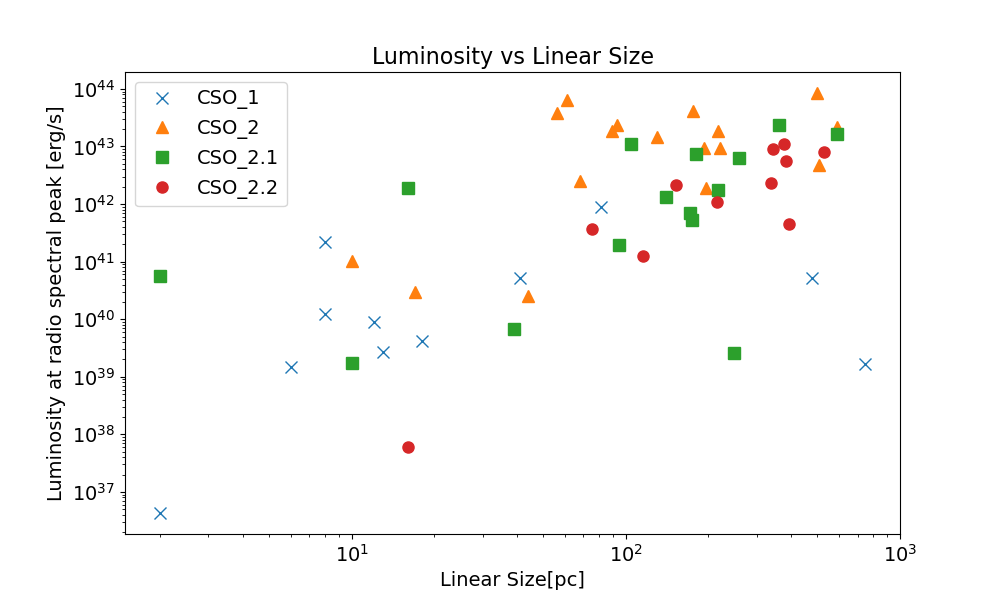
\includegraphics[width=.8\textwidth]{C:/Users/henri/OneDrive/Documents/NTNU/Semester 10/Masteroppgave/Plots/Lin_size_vs_Luminosity.png}
    \caption{The radio luminosity at peak frequency of CSOs as a function of linear size.}
    \label{fig:Luminosity_size}
\end{figure}

The figure shows a distinction between CSO $2.0$ and the other classes where CSO $2.0$ have a higher luminosity at peak frequency compared to the other classes of similar sizes. In addition one sees a trend of higher luminosity at the peak frequency for larger sources. This is expected since the amount of energy deposited into the lobes will 
 affect the size of the lobes.

One can also investigate the relation between redshift and luminosity at peak frequency as seen in figure \ref{fig:Luminosity_redshift}. Here one sees a trend of higher luminosity at peak frequency for higher redshifts, indicating a possible obersvation bias for longer distances.



\begin{figure}
    \centering
    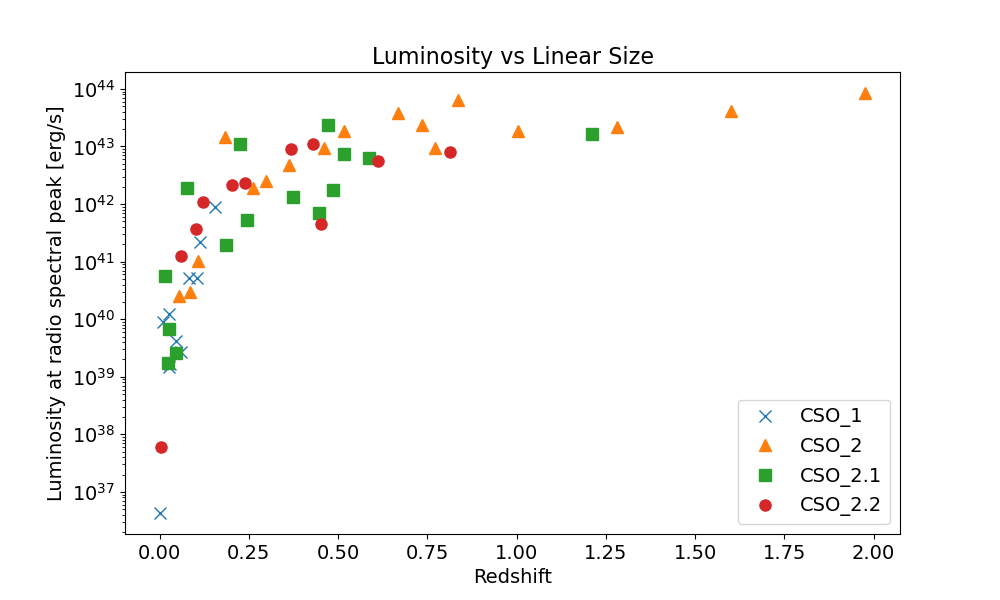
\includegraphics[width=.8\textwidth]{C:/Users/henri/OneDrive/Documents/NTNU/Semester 10/Masteroppgave/Plots/z_vs_Luminosity.png}
    \caption{The radio luminosity at peak frequency of CSOs as a function of redshift.}
    \label{fig:Luminosity_redshift}
\end{figure}
\subsection{Prevalence of CSOs}







%\subsection{Stability in jet expansion and lobes.} The most promesing feature of CSOs which we will see as a key feature in the section on time-scales is the stability of the lobes in radio emission, the stability of the jet expansion and the stability of most wavelengths in emissions. In \cite{bronzini2024investigating} they report no significant variablilty of one CSO source in gamma rays, variability of the order of years in x-ray, with the broadband SED showing variability on the timescales of years. This is a clear distincsion from other jetted AGN which are known to be highly variable. Having stable systems allows for more efficient acceleration of ions, and significantly increases the possibility of producing UHECRs. 
\newpage

\chapter{CSO as sources of UHECRs and neutrinos}
\section{CSO as sources of UHECRs and neutrinos}
\subsection{Magnetic field strength}
%In order to estimate magnetic field strength one outlines two methods in section \ref{sec:equipartition} and \ref{sec:SSA}. Now one only needs to collect data. Of the two methods, the equipartition method is the most reliable and the easiest to collect data for, but uses the assumtion of equipartition, and assumption that is not necessarly the case. The SSA method is more difficult to obtain data for, due to the necessatiy of collecting data at the correct frequency, but does not need an assumption between the magnetic field strength and the energy density of the particles. In addition to this both values will work as great cross checks for different parameters in the system. For Synchrotron self absorption(SSA) $B \propto R^{4}$, while for equipartition $B \propto R^{-2/7}$.

%From table \ref{tab:CSO_sources} one is given the turnover frequency and its corresponding flux density. The problem here is that this value is for the entire source and not any hotspot or lobe. In order to derive the appropriate value one needs to know the size of a lobe, and importantly the fraction of emitted radiation that stem from that lobe compared to the rest of the source. This is a difficult task ridden with selection bias, but one will make an effort to estimate the magnetic field strength. In order to estimate both the SSA and equipartition magnetic field one will turn to a catalogue of 374 strong flat spectrum radio sources, called The VSOP 5 GHz Continuum Survey: The Pre-launch VLBA Observations, \cite{nrao1996}. This catalogue measured high resolution radio images of some  sources contained in table \ref*{tab:CSO_sources} at $5$GHz. These images will allow us to estimate the size of an individual lobe, here we chose the most powerful lobe, and the fraction of the total flux density that comes from this lobe. The same fraction will then be applied to the turnover flux density given in table \ref{tab:CSO_sources} to estimate the turnover flux density from this lobe. Additionally, the NRAO catalogue gives also flux densities measured at $5$GHz allowing us to estimate the equipartition magnetic field strength based on an assumption of the spectral index. One finds an overlap of $10$ sources between the two catalogues, and the extracted values can be found in table \ref{tab:CSO_B}.

In order to estimate magnetic field strength, one outlines two methods in section \ref{sec:equipartition} and \ref{sec:SSA}. Now one only needs to collect data. Of the two methods, the equipartition method is the most reliable and the easiest to collect data for, but uses the assumption of equipartition, an assumption that is not necessarily the case. The SSA method is more difficult to obtain data for, due to the necessity of collecting data at the correct frequency, but does not need an assumption between the magnetic field strength and the energy density of the particles. In addition to this, both values will work as great cross-checks for different parameters in the system. For Synchrotron Self-Absorption (SSA) $B \propto R^{4}$, while for equipartition $B \propto R^{-2/7}$.

From table \ref{tab:CSO_sources} one is given the turnover frequency and its corresponding flux density. The problem here is that this value is for the entire source and not any hotspot or lobe. In order to derive the appropriate value, one needs to know the size of a lobe, and importantly the fraction of emitted radiation that stems from that lobe compared to the rest of the source. This is a difficult task ridden with selection bias, but one will make an effort to estimate the magnetic field strength. In order to estimate both the SSA and equipartition magnetic fields, one will turn to a catalogue of 374 strong flat spectrum radio sources, called The VSOP 5 GHz Continuum Survey: The Pre-launch VLBA Observations, \cite{nrao1996}. This catalogue measured high-resolution radio images of some sources contained in table \ref*{tab:CSO_sources} at $5$GHz. These images will allow us to estimate the size of an individual lobe, here we chose the most powerful lobe, and the fraction of the total flux density that comes from this lobe. The same fraction will then be applied to the turnover flux density given in table \ref{tab:CSO_sources} to estimate the turnover flux density from this lobe. Additionally, the NRAO catalogue also gives flux densities measured at $5$GHz, allowing us to estimate the equipartition magnetic field strength based on an assumption of the spectral index. One finds an overlap of $10$ sources between the two catalogues, and the extracted values can be found in table \ref{tab:CSO_B}.


\begin{table}
    \centering
    \begin{tabular}{|c|c|c|c|c|c|c|c|}
    \hline
    \textbf{Name} & \textbf{z} & \textbf{Class} & \textbf{$\nu_t$} & \textbf{$S_{\nu_t}$} & \textbf{$\nu_{5GHz}$} & \textbf{$\theta_{lobe}$} & \textbf{$S_{\nu_{5GHz}}$} \\
    \hline
    J0029+345 & 0.517 & 2.0 & 0.8 & 1.178 & 5 & 2.1 & 0.766 \\
    J0111+3906 & 0.66847 & 2.0 & 4.0 & 0.88189 & 5 & 0.95 & 0.862 \\
    J0119+3210 & 0.0602 & 2.2 & 0.4 & 0.5125 & 5 & 9.85 & 0.205 \\
    J0405+3803 & 0.055 & 2.0 & 0.07 & 2.554 & 5 & 2.7 & 0.418 \\
    J0713+4349 & 0.518 & 2.0 & 1.9 & 0.94311 & 5 & 1.45 & 0.722 \\
    J1035+5628 & 0.0460 & 2.0 & 1.3 & 1.0659 & 5 & 1.6 & 0.741 \\
    J1158+2450 & 0.203 & 2.2 & 2 & 0.588 & 5 & 4 & 0.566 \\
    J1347+1217 & 0.121 & 2.2 & 0.4 & 1.3947 & 5 & 1 & 0.488 \\
    J1407+2827 & 0.077 & 2.1 & 4.9 & 2.9375 & 5 & 1.2 & 2.350 \\
    J2022+6136 & 0.2266 & 2.1 & 4.086 & 1.57256 & 5 & 2 & 1.787 \\
    J2355+4950 & 0.238 & 2.2 & 0.7 & 1.5450 & 5 & 1.8 & 0.791 \\
    \hline
    \end{tabular}
    \caption{Overlapping sources between the NRAO catalogue and \cite{kiehlmann2023compact} and the extracted values scaled to represent one lobe hotspot.}
    \label{tab:CSO_B}
\end{table}

From here one can estimate the magnetic fields via both methods. 

\begin{figure}
    \centering
    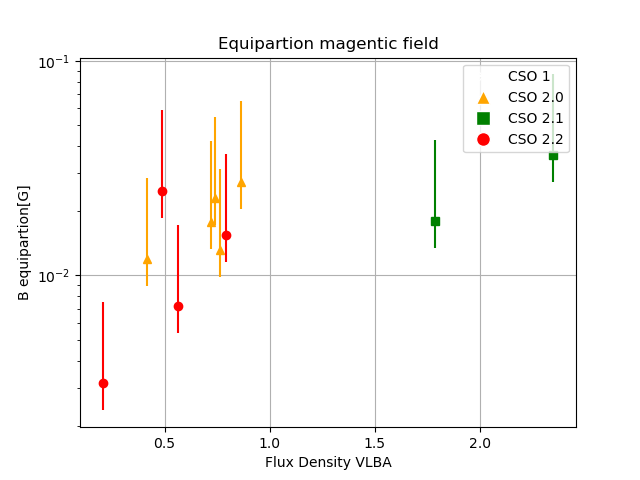
\includegraphics[width=0.8\textwidth]{C:/Users/henri/OneDrive/Documents/NTNU/Semester 10/Masteroppgave/Plots/Equipartion.png}
    \caption{Magnetic field strength estimated from the equipartition method. The errobars are calculated from the span of values obtained from different spectral index ranging from $0.6$ to $1.3$.}
    \label{fig:B_field}
\end{figure}

\begin{figure}
    \centering
    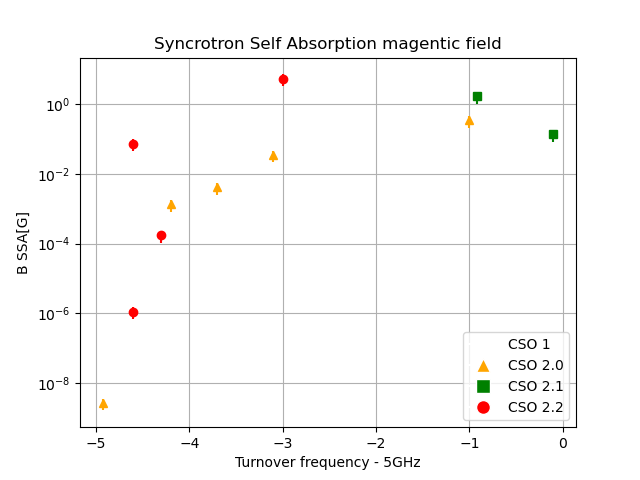
\includegraphics[width=0.8\textwidth]{C:/Users/henri/OneDrive/Documents/NTNU/Semester 10/Masteroppgave/Plots/SSA.png}
    \caption{Magnetic field strength estimated from the SSA method. The errobars are calculated from the span of values of $b(\alpha)$ obtained from different optical thickness. $b(\alpha)$ ranges from $1.08$ to $2.38$.}
    \label{fig:B_field_SSA}
\end{figure}

%The result of the magnetic field estimations are a little varied, but the most reliable numbers is a magnetic fields strenght between $5 \times 10^{-3}$ and $1 \times 10^{-1}$ G. Here one relies most heavilly on the equipartition argument due to the SSA estimation being very biased, as the estimation of the lobe size is wrong for turnover frequencies lower than the imaging. The lobe size estimation is based on the images from the $5$ GHs survey, and as one sees in figure \ref{fig:B_field_SSA} the magnetic field strenght from SSA calculations is heavilly dependent on the different between the turnover frequency and the frequency of the observation. The SSA still give values for the magnetic field strength that are in the same order of magnitude as the equipartition method at turnover frequencies closer to the measured frequency and even go above.

%The equipartition calculations is also greatly affected by the choice of spectral index, as seen by the large errorbars, but places the sources neatly in the same order of magnitude as the best SSA calculations. For SSA calculations that go above the equipartition values one can have several explinations. Firstly it could be that the equipartition argument does not hold and that the magnetic field is stronger than the equipartition value, this can be investigated by looking at jet power. Secondly it could be that there are other factors than synchrotron self absorption that make the source optically dense. If one includes free-free absorption one could shift the turnover frequency to a higher value, resulting in a higher magnetic field measurement. This is not investigated in this work, but is a possible explanation for the high magnetic field strength. For the continued work in this thesis one will use the equipartition magnetic field strength as the most reliable value, but will also consider the SSA magnetic field strength as a possible value. The general magnetic field of a CSO in all classes would then be $B = 10^{-2}$ G. 

%The estimation of the radius of our emitting regions in the previous section can be put under question. In order the estimate the precise value of our emitting regions one would idealy measure the flux at the turnover frequency in order for the most flux not to drop under the sensitivity of the telescope. Even given this \cite{1983ApJ...264..296M} would estimate the angular size of the source is still $\theta_{\text{true}} = 1.8\times \theta_{\text{FWHM}}$. For some sources in table \ref{tab:CSO_B} one measures close to the turnover frequency, but for most a more thorough consideration could be in order. The equipartition method is not as sensitive to the size of the source, but one should still be careful not taking the values at face value.

%In order to do so, another method of estimating the radius of our lobes is outlined in \cite{W_jtowicz_2020}. They uses a relation between the total linear size of an objects and the estimated relations between the semi-major axis and the semi-minor axis. The argument is that CSOs have relativly large aspect rations between their axis, with an estimation equaling $b/a \approx 0.25$. From this they introduce the effective radius of the radio lobes via 


The result of the magnetic field estimations is a little varied, but the most reliable numbers indicate a magnetic field strength between $5 \times 10^{-3}$ and $1 \times 10^{-1}$ G. Here, one relies most heavily on the equipartition argument due to the SSA estimation being very biased, as the estimation of the lobe size is wrong for turnover frequencies lower than the imaging. The lobe size estimation is based on the images from the $5$ GHz survey, and as one sees in figure \ref{fig:B_field_SSA}, the magnetic field strength from SSA calculations is heavily dependent on the difference between the turnover frequency and the frequency of the observation. The SSA still gives values for the magnetic field strength that are in the same order of magnitude as the equipartition method at turnover frequencies closer to the measured frequency and even go above.

The equipartition calculations are also greatly affected by the choice of spectral index, as seen by the large error bars, but place the sources neatly in the same order of magnitude as the best SSA calculations. For SSA calculations that go above the equipartition values, one can have several explanations. Firstly, it could be that the equipartition argument does not hold and that the magnetic field is stronger than the equipartition value; this can be investigated by looking at jet power. Secondly, it could be that there are other factors than synchrotron self-absorption that make the source optically dense. If one includes free-free absorption, one could shift the turnover frequency to a higher value, resulting in a higher magnetic field measurement. This is not investigated in this work but is a possible explanation for the high magnetic field strength. For the continued work in this thesis, one will use the equipartition magnetic field strength as a reliable lower value but will also consider the SSA magnetic field strength as a possible value. %The general magnetic field of a CSO in all classes would then be $B = 10^{-2}$ G.

The estimation of the radius of our emitting regions in the previous section can be put under question. In order to estimate the precise value of our emitting regions, one would ideally measure the flux at the turnover frequency in order for the most flux not to drop under the sensitivity of the telescope. Even given this, \cite{1983ApJ...264..296M} would estimate the angular size of the source is still $\theta_{\text{true}} = 1.8\times \theta_{\text{FWHM}}$. For some sources in table \ref{tab:CSO_B}, one measures close to the turnover frequency, but for most, a more thorough consideration could be in order. The equipartition method is not as sensitive to the size of the source, but one should still be careful not to take the values at face value. 

The biggest problem with SSA method for lower turnover frequencies is that one might underestimate 


%with this estimation one can estimate the size of the lobes for the sources in table \ref{tab:CSO_B}, and compare the resulting values to the radii obtained from the FWHM of the images in the NRAO catalogue.  here one will note that this is an estimation of lobe size and not necessarly the hotspot which we are interested in. The results 



%\subsection{Energy budget}
%Via the energy budget of the CSOs, one can get an idea of where it is possible to accelerate protons to UHECR energies. The most natural place is in the Hillas diagram, where one can compare the size and magnetic field strength of the system to the maximum energy of the proton. From our magnetic field estimations one can see that the magnetic field strength is between $10^{-2}$ and $1$ G. The radius of our emitting region is from the order of $2$ pc to $10$ pc when the lobe expands. It would be reasonable to assume that as the lobe expands the magnetic field strength decreases, but as it expands more energy is also being fed into the hot spots, therefore one will could assume a magnetic field strength of $10^{-1}$ G for the biggest lobes as well. The choice of magnetic field strength and radius of the emitting region can be compared to other candidates for emitters and is shown in figure \ref{fig:Hillas}.
With this estimation, one can estimate the size of the lobes for the sources in table \ref{tab:CSO_B}, and compare the resulting values to the radii obtained from the FWHM of the images in the NRAO catalogue. Here, one will note that this is an estimation of lobe size and not necessarily the hotspot which we are interested in. The results...

\subsection{Energy budget}
Via the energy budget of the CSOs, one can get an idea of where it is possible to accelerate protons to UHECR energies. The most natural place is in the Hillas diagram, where one can compare the size and magnetic field strength of the system to the maximum energy of the proton. From our magnetic field estimations, one can see that the magnetic field strength is between $10^{-2}$ and $1$ G. The radius of our emitting region is on the order of $2$ pc to $10$ pc when the lobe expands. It would be reasonable to assume that as the lobe expands, the magnetic field strength decreases, but as it expands, more energy is also being fed into the hotspots. Therefore, one could assume a magnetic field strength of $10^{-1}$ G for the biggest lobes as well. The choice of magnetic field strength and radius of the emitting region can be compared to other candidates for emitters and is shown in figure \ref{fig:Hillas}.


\begin{figure}
    \centering
    \includegraphics[width=0.8\textwidth]{C:/Users/henri/OneDrive/Documents/NTNU/Semester 10/Masteroppgave/Plots/hillas.png}
    \caption{Hillas diagram for the CSO. The red line represents the maximum energy of the proton that can be accelerated in the system, and blue is the same just for Iron. }
    \label{fig:Hillas}
\end{figure}

%From the figure it becomes clearer that CSO is a class worthy of being investigated further, both their lobe size, and their magnetic field strength make them great candidates. As for all potential sources one observes one needs a highly efficient acceleration mechanism in order to accelerate the protons. The efficiency of acceleration is described by the $\beta$ factor in figure \ref*{fig:Hillas}. The CSO hotspots separate themselves from usual AGN hotspots which are attributed to large lobes at the end of the jet in huge radio galaxies. The more compact hotspots in CSOs might be more efficient in accelerating protons, but this needs to be looked into further.  
\subsubsection{x-ray power}
%In stduies such as \cite{Jacobsen:2015mga} and \cite{10.1111/j.1745-3933.2008.00499.x} one discuss the possibility of using the x-ray flux or hard x-ray flux as a proxy for hadronic acceleration. This is a common start in trying to probe the biggest emitters of neutrinoes and UHECRs, and it is worth looking at CSOs this way as well. The biggest caveat with this method is that one usually attributes the x-ray flux to the core region, and then one might have different mechanisms for acceleration than one has in the hotspots. In the case of our model of a CSO SED one immeditly sees that the total x-ray flux from the x-ray corona will be a factor of the total accretion luminosity. For our model of timescales later in the chapter one assumes the fraction to be $f_X = 0.3$. and for this one recived a typical total x-ray corona flux of $3 \times 10^{42} $erg/s. This number is quite a lot higher than  what was found by  \cite{bronzini2024investigating} who using two spectral models, found a x-ray flux for two compact sources, PKS 1718-649 and TXS 1146+596, to be just shy of $10^{41}$ erg/s. In addition to this estimate \cite{W_jtowicz_2020} cites the x-ray flux of 17 CSOs and here one will do another cross correlation with the CSOs in table \ref*{tab:CSO_sources}. The results can be seen in table \ref{tab:CSO_xray}.
From the figure, it becomes clearer that CSOs are a class worthy of being investigated further; both their lobe size and their magnetic field strength make them great candidates. As with all potential sources, one observes that a highly efficient acceleration mechanism is needed to accelerate the protons. The efficiency of acceleration is described by the $\beta$ factor in figure \ref*{fig:Hillas}. The CSO hotspots separate themselves from usual AGN hotspots, which are attributed to large lobes at the end of the jet in huge radio galaxies. The more compact hotspots in CSOs might be more efficient in accelerating protons, but this needs to be looked into further.

\subsubsection{X-ray power}
In studies such as \cite{Jacobsen:2015mga} and \cite{10.1111/j.1745-3933.2008.00499.x}, one discusses the possibility of using the X-ray flux or hard X-ray flux as a proxy for hadronic acceleration. This is a common start in trying to probe the biggest emitters of neutrinos and UHECRs, and it is worth looking at CSOs this way as well. The biggest caveat with this method is that one usually attributes the X-ray flux to the core region, and then one might have different mechanisms for acceleration than one has in the hotspots. In the case of our model of a CSO SED, one immediately sees that the total X-ray flux from the X-ray corona will be a factor of the total accretion luminosity. For our model of timescales later in the chapter, one assumes the fraction to be $f_X = 0.3$, and for this, one received a typical total X-ray corona flux of $3 \times 10^{42}$ erg/s. This number is quite a lot higher than what was found by \cite{bronzini2024investigating}, who, using two spectral models, found an X-ray flux for two compact sources, PKS 1718-649 and TXS 1146+596, to be just shy of $10^{41}$ erg/s. In addition to this estimate, \cite{W_jtowicz_2020} cites the X-ray flux of 17 CSOs, and here one will do another cross-correlation with the CSOs in table \ref*{tab:CSO_sources}. The results can be seen in table \ref{tab:CSO_xray}.


\begin{table}
    \centering
    \begin{tabular}{|c|c|c|c|}
        \hline
        \textbf{Name} & \textbf{z} & \textbf{Class} &   \textbf{$L_{\text{X-ray}}$} \\
        \hline

        

        J0111+3906 & 0.66847 & 2.0 & 70 \\
        J0119+3210 & 0.0602 & 2.2 & $<$1.0 \\
        J0713+4349 & 0.518 & 2.0 & 394 \\
        J1511+0518 & 0.084 & 2.0 & 30 \\
        J1939-6342 & 0.183 & 2.0 & 6 \\
        J1944+5448 & 0.263 & 2.0 & 7.31 \\
        J1945+7055 & 0.101 & 2.2 & 12 \\ 
        J2022+6136& 0.227 & 2.1 & 112 \\
        J2355+4950 & 0.238 & 2.2 & 13 \\
        \hline
    \end{tabular}
    \caption{X-ray flux of the CSOs in table \ref{tab:CSO_sources} found in the data set in \cite{W_jtowicz_2020}. The X-flux is given in units of $10^{42}$ erg/s.}
\label{tab:CSO_xray}
\end{table}

%After cross correlation one is left with $9$ objects that are in both catalogues. The X-ray flux of these objects span the range between $6-394 \times 10^{42}$ erg/s for CSO $2.0$ which has the most data. CSO 2.2 with three data points does not have any that exceed $13 \times 10 ^{42}$ erg/s and the lone CSO $2.1$ sits at a powerful $112\times 10^{42}$erg/s. With these values one can compare them to other jetted AGN like Bl lacs and blazars. One will do this by looking at the total x-ray emissivity of the sources and compare it to the local emissivity of the UHECRs. The total x-ray emissivity is given by $Q_{\text{X-ray}} = L_{\text{X-ray}} n_{\text{CSO}}$. The results can be seen in figure \ref{fig:X-ray_em}. The amount of data collect is very low and one can not make any strong conclusions from this, but using the values as a benchmark value one can see that the x-ray emissivity of the CSO $2.0$ and $2.1$ span a sizeable area above the local emissivity of UHECRs and neutrinos.  CSO $2.2$ seem to emit X-ray at a lower rate but still powerful enough to exceed the local emissivity of UHECRs. In previous work I have found that even though the X-ray flux is a good indicator of relativisitc particles, in most cases electrons, there still is work to be done relating it to UHECRs and neutrino. Given that the X-ray flux of the CSOs surpass the local emissivity of UHECRs and neutrinos significantly one can say that the CSOs are also good candidates for UHECRs and neutrino production when compared to other AGN. 

After cross-correlation, one is left with $9$ objects that are in both catalogues. The X-ray flux of these objects spans the range between $6-394 \times 10^{42}$ erg/s for CSO $2.0$, which has the most data. CSO 2.2, with three data points, does not have any that exceed $13 \times 10^{42}$ erg/s, and the lone CSO $2.1$ sits at a powerful $112 \times 10^{42}$ erg/s. With these values, one can compare them to other jetted AGN like BL Lacs and blazars. One will do this by looking at the total X-ray emissivity of the sources and comparing it to the local emissivity of the UHECRs. The total X-ray emissivity is given by $Q_{\text{X-ray}} = L_{\text{X-ray}} n_{\text{CSO}}$. The results can be seen in figure \ref{fig:X-ray_em}. 

The amount of data collected is very low, and one cannot make any strong conclusions from this, but using the values as a benchmark, one can see that the X-ray emissivity of the CSO $2.0$ and $2.1$ spans a sizeable area above the local emissivity of UHECRs and neutrinos. CSO $2.2$ seems to emit X-ray at a lower rate but still powerful enough to exceed the local emissivity of UHECRs. In previous work, I have found that even though the X-ray flux is a good indicator of relativistic particles, in most cases electrons, there still is work to be done relating it to UHECRs and neutrinos. Given that the X-ray flux of the CSOs surpasses the local emissivity of UHECRs and neutrinos significantly, one can say that the CSOs are also good candidates for UHECRs and neutrino production when compared to other AGN.



\begin{figure}[ht]
    \centering
    \begin{subfigure}[b]{0.49\textwidth}
        \centering
        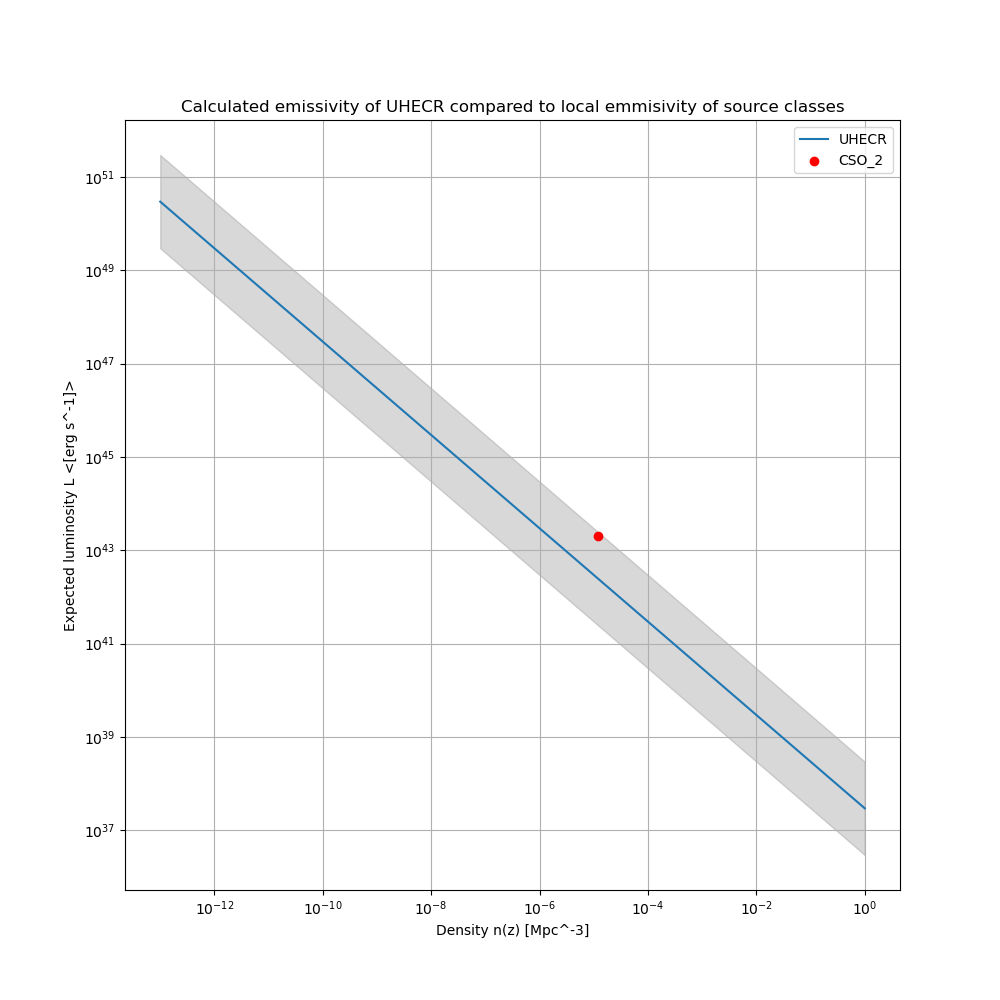
\includegraphics[width=\textwidth]{C:/Users/henri/OneDrive/Documents/NTNU/Semester 10/Masteroppgave/Plots/L_n_uhecr_calc_cso.png}
        \caption{UHECRs emissivity compared to X-ray luminosity of 
        AGN classes }
        \label{fig:uhecr_em}
    \end{subfigure}
    \hfill
    \begin{subfigure}[b]{0.49\textwidth}
        \centering
        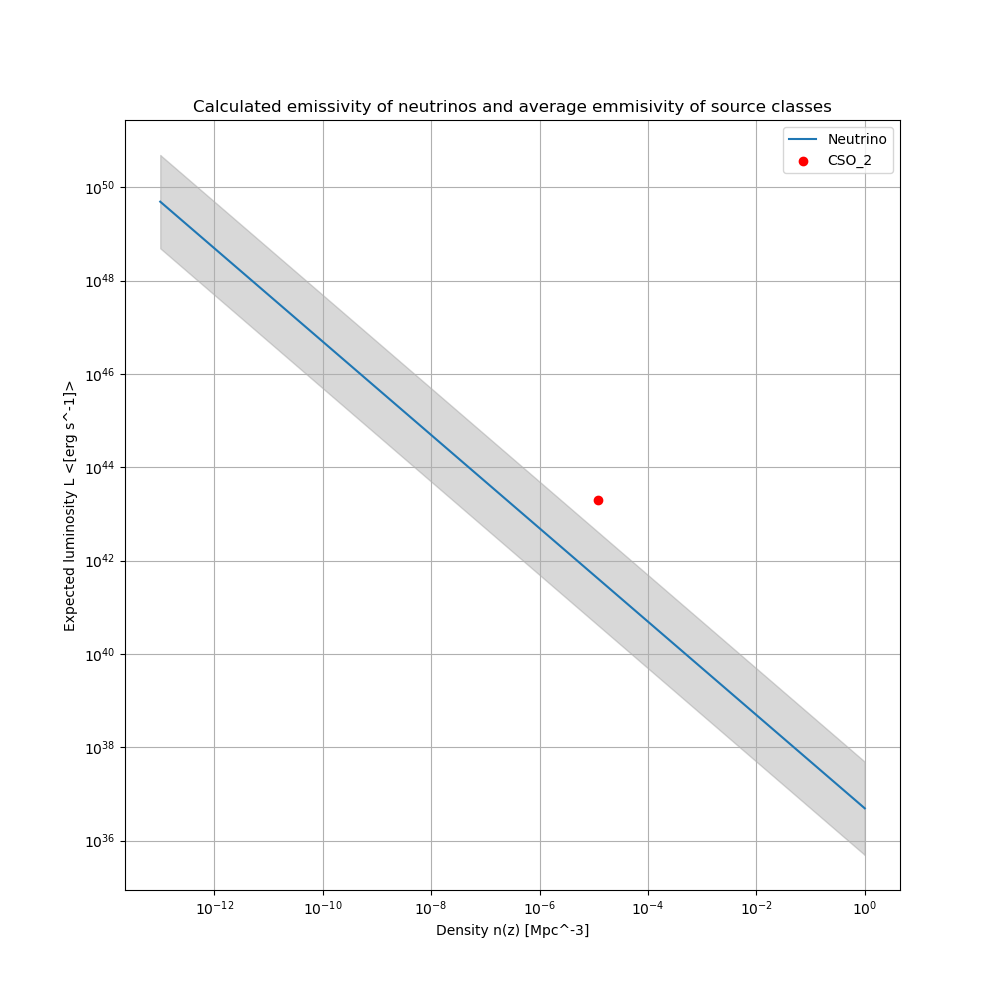
\includegraphics[width=\textwidth]{C:/Users/henri/OneDrive/Documents/NTNU/Semester 10/Masteroppgave/Plots/L_n_neut_calc_cso.png}
        \caption{Neutrinos emissivity compared to X-ray luminosity of AGN classes}
        \label{fig:neut_em}
    \end{subfigure}
    %\caption{Neutrinos emissivity compared to X-ray luminosity of CSO classes }
    \label{fig:X-ray_em}
\end{figure}


\subsubsection{Radio power}



\subsubsection{Jet power}
%The jet power of jetted AGN can be an important parameter in constraining parameters such as particle energy density, and as one will argue if one can move away from equipartition. If the jet energy is carried by particles one can relate the comoving particle density to the stationary frame jet power $P_j$ as, 



%This is for a two sided jet, where $\Omega_j$ is the jet opening angle in sr. The jet power relation here includes the assumption that the jet is carried by electrons, and that the jet power is related to the bulk Lorentz factor of the plasma outflow. By using a general particle distribution for electrons for example as seen in equation \ref{eq:proton_spectrum} and including a factor to account for kinetic energy being carried by protons one can represent the jet power as a function of the kinetic energy carried by particles. One adds to this the power required to expel magnetic field laden plasma given as



%By now including the equipartion magnetic field $B_{\text{eq}}$ and rewriting the kinetic terms as done in section \ref{sec:equipartition}  one can relate the minimum jet power as a function of the equipartion magnetic field. One is skipping a few steps of derivation, but this can be found in \cite{BHradiation} on page 136. The result is the minimum jet power of the system as a function of the equipartition magnetic field strength given as

The jet power of jetted AGN can be an important parameter in constraining parameters such as particle energy density, and as one will argue, if one can move away from equipartition. If the jet energy is carried by particles, one can relate the comoving particle density to the stationary frame jet power $P_j$ as,

\begin{equation}
    \frac{P_j}{2\Omega_j R^2 c \beta (\Gamma m_e c^2)}
\end{equation}

This is for a two-sided jet, where $\Omega_j$ is the jet opening angle in sr. The jet power relation here includes the assumption that the jet is carried by electrons and that the jet power is related to the bulk Lorentz factor of the plasma outflow. By using a general particle distribution for electrons, for example, as seen in equation \ref{eq:proton_spectrum} and including a factor to account for kinetic energy being carried by protons, one can represent the jet power as a function of the kinetic energy carried by particles. One adds to this the power required to expel magnetic field-laden plasma given as

\begin{equation}
    P_b = 2 \frac{B^2}{8\pi} \Omega_j R^2 c \beta \Gamma^2
\end{equation}

By now including the equipartition magnetic field $B_{\text{eq}}$ and rewriting the kinetic terms as done in section \ref{sec:equipartition}, one can relate the minimum jet power as a function of the equipartition magnetic field. One is skipping a few steps of derivation, but this can be found in \cite{BHradiation} on page 136. The result is the minimum jet power of the system as a function of the equipartition magnetic field strength given as

\begin{equation}
    P_j(B_{\text{eq}}) = \frac{14}{3}\pi c \beta \Gamma^2 R^2 \frac{B_{\text{eq}}^2}{8 \pi}
\end{equation}


The last quantities that need to be estimated are the bulk Lorentz factor and, importantly, jet $\beta$, or the speed of expansion into the surrounding medium. The bulk Lorentz factor of our jet is estimated to be $\Gamma < 1.1$ since CSO jets are not relativistically beamed. The last value is the expansion speed of the jet, which will vary from class to class. In the case of CSO $2.0$, one will estimate a value of $\beta$ between $0.1 - 0.4$ c. In \cite{sullivan2024smallscale}, they cite the expansion speed of a CSO $2.0$ to be approximately $200 \times c_s = 200 \times 250$ km/s, where $c_s$ is the sound speed. This gives a value of $\beta = 0.166$ c. Part of the definition of CSO $2.1$ is that the jet is decelerating, and therefore one would expect $\beta$ to lie between $0.1$ and $8\times 10^{-4}$ c. Lastly, the speed of the jet in CSO $2.2$ is by definition extremely low or non-existent, where the apparent motion of emitting bubbles is due to adiabatic expansion. Therefore, one argues that the speed of any emitting blob is to move at the speed of sound in the medium, and therefore $\beta = 8\times 10^{-4}$ c. For values of jet energy derived this way, one will argue that they mostly will work for CSO $2.0$ due to the fact that their jet opening angle has not evolved greatly from their initial state.

One will need to compare this jet power to another method in order to investigate the underlying dynamics. In \cite{Blandford_1977}, one finds a relation between the jet power and the accretion rate of the system. The relation is given as

\begin{equation}
    P_j = k \dot{M} c^2
\end{equation}

where $k$ is a constant that depends on the rotation velocity of the system's black hole. The various values of $k$ range from $0.3$ to $2$, where $k=2$ represents a maximally spinning black hole, $\Omega_{\text{max}} = c^3/2GM$. One can estimate the accretion rate as a fraction of the X-ray luminosity via some simple assumptions. Like our broadband SED modeling, one assumes that the X-ray luminosity is a fraction of our accretion luminosity $L_{\text{X-ray}} = f_X L_{\text{d}}$. The accretion rate is given as $L_{\text{d}} = \eta \dot{M} c^2$ where $\eta$ is the efficiency of the accretion disk. By substituting the mass accretion rate as a function of the X-ray luminosity, one can get a simple estimate for the jet power. The resulting jet power is given as

\begin{equation}
    \label{eq:jet_power}
    P_j = \frac{k}{\eta f_X} L_{\text{X-ray}} = \alpha L_{\text{X-ray}}
\end{equation}

Here, $\alpha$ is a constant that absorbs the other constants since they are most likely dependent on each other. One will utilize the same table as before to estimate the jet power of the CSOs, but one needs to define the equipartition magnetic field for them as well. Since one does not have NRAO data for these sources, one will use the relation between linear size and radius to estimate the radius of the lobes. Otherwise, $S_v$ is given in \cite{W_jtowicz_2020} with the corresponding X-ray luminosity. The jet power can then be seen in figure \ref{fig:jet_power}.


\begin{figure}
    \centering
    \includegraphics[width=0.8\textwidth]{C:/Users/henri/OneDrive/Documents/NTNU/Semester 10/Masteroppgave/Plots/jet_power.png}
    \caption{Jet power of the CSOs in table \ref{tab:CSO_sources}. The jet power is calculated using the minimum jet power argument based on magnetic field equipartition. The bars in line with each line represent the estimated jet power based on the X-ray luminosity varying the value of $\alpha$ in equation \ref{eq:jet_power}.} While the line representing minimum jet power is varying based on $\beta$ values. 
    \label{fig:jet_power}
\end{figure}

It becomes clear that the gap between X-ray flux and CSO $2.2$s is too large to account for the jet power of the system. This is not surprising since all X-ray flux measured is attributed to the core region but this will likely not be the case. As seen in the SED figure \ref{fig:SED_sep} the x-ray flux can have multiple sources, of which upscattering by relativistic electrons happening outside the x-ray corona is very likely. Therefore, this comparisson has some big caveat when it comes to X-ray estimated jet power. On the other hand The minimum jet powers of CSO$2.0$ and $2.1$ are more inline with the power estimated via the X-ray luminosity. This might indicate that more of the x-ray flux from these sources is related to the x-ray core, and our assumption of the x-ray flux being a proxy for jet power is more valid. 


\subsection{Time scales }
Looking at characteristic timescales for CSOs is a powerful tool for understanding the maximum energy that can be obtained from the system. In section 4, one outlined the general method, and here one will present the results for CSO 2s.

With given data obtained from measurements, one will define conservative estimates for an acceleration region in the CSO. The regions of interest are the hotspots created during the CSO 2.0 and 2.1 stages, and one will observe that these are good regions for acceleration. The first constant that needs to be estimated is the size of our emitting system. From observations, it is clear that the radio lobes expand significantly during the CSO lifetime. From radio variations, which are on the order of tens of years, a reasonably conservative estimate for the size of the lobes is $R_{\text{lobe}} = 2$ pc. In addition to this size requirement, one will also include the lifetime of the source, which is on the order of $10^3$ years.

In estimating the magnetic field strength, one found the values of typical lobes to be $B = 10^{-2}$ G from the equipartition argument. This value has been found before in previous literature and is a reasonable lower limit for the magnetic field strength. It is important to note that the magnetic field strength is a very important parameter and yet bears significant uncertainty. It may very well be that the magnetic field strength is higher than this value, and one will discuss this in the following sections.

For the photopion production, one will use the photon field as described in section 4, where the used parameters can be found in table \ref{tab:SED_params}. This field is based on the field of a much larger AGN, but one assumes for this discussion that the field is similar in the CSO. One can compare this generated field to the ones presented in \cite{bronzini2024investigating}, where they find a similar magnitude and shape of the resulting SED. A significant note is that the field is also not strongly beamed, giving room for other parts of AGNs to be seen. The resulting SED is seen in figure \ref{fig:SED_sep}. The exact shape of the SED is not incredibly important for the following discussion, but the broad shape and magnitude are important. The exact shape of the SED will become more important when one starts looking for observational signatures of the acceleration, such as gamma rays, and here one can use the model SED and minimize the parameter space to find the best fit.


\begin{figure}
    \centering
    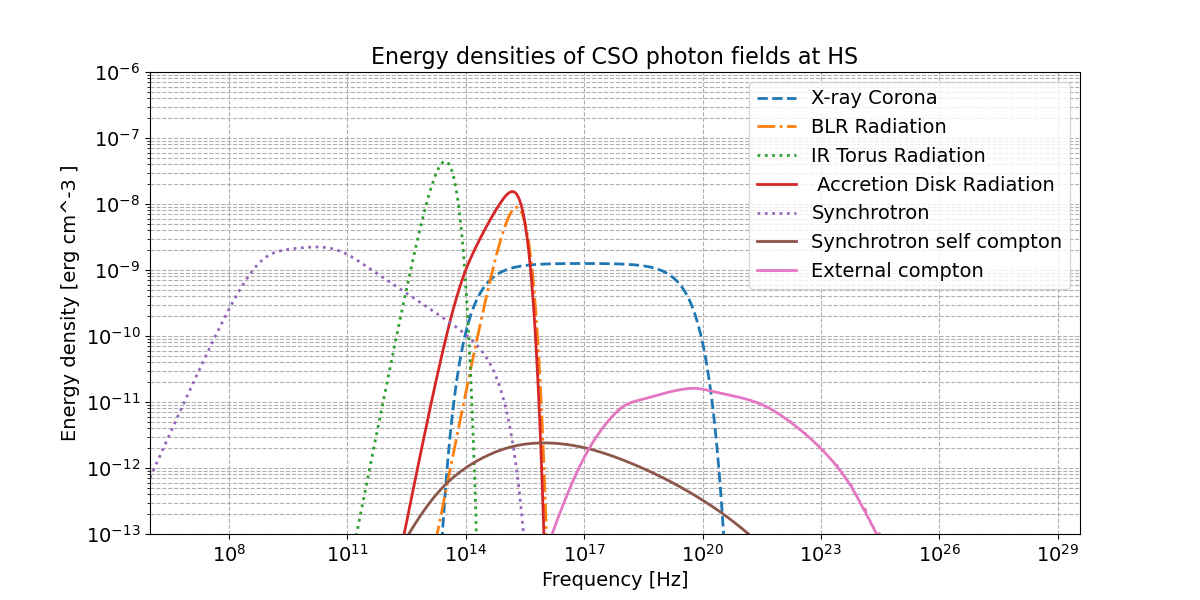
\includegraphics[width=0.8\textwidth]{C:/Users/henri/OneDrive/Documents/NTNU/Semester 10/Masteroppgave/Plots/SEDs_sep.png}
    \caption{SED of the different regions in the CSO. The SED is based on the parameters in table \ref{tab:SED_params}.}
    \label{fig:SED_sep}
\end{figure}





\begin{table}
    \centering
    \begin{tabular}{|c|c|}
        \hline
        Parameter & Value \\
        \hline
        $L_{d}$ & $10^{43}$ erg/s \\
        $GM$ & $G 10^{8} M_{\odot}$ \\
        $RS$ & $\frac{2GM}{c^2}$ \\
        $\eta$ & 0.1 \\
        $f_{X}$ & 0.3 \\
        $R_{X}$ & 30$ RS $\\
        $\beta$ & 0.4 $c$\\
        $f_{\text{BLR}}$ & 0.1 \\
        $R_{\text{BLR}}$ & $10^{17} \sqrt{L_{d}/10^{45}}$ cm \\
        $f_{\text{IR}}$ & 0.5 \\
        $R_{\text{IR}}$ & $2.5 10^{18}\sqrt{L_{d}/10^{45}}$ cm \\
        $\Gamma$ & 1.1 \\
        \hline
    \end{tabular}
    \caption{Parameters used to determine the SED of the different regions.}
    \label{tab:SED_params}
\end{table}


From the above parameters one can estimate the characteristic timescales for the CSO, seen in figure \ref{fig:timescales}. 

\begin{figure}
    \centering
    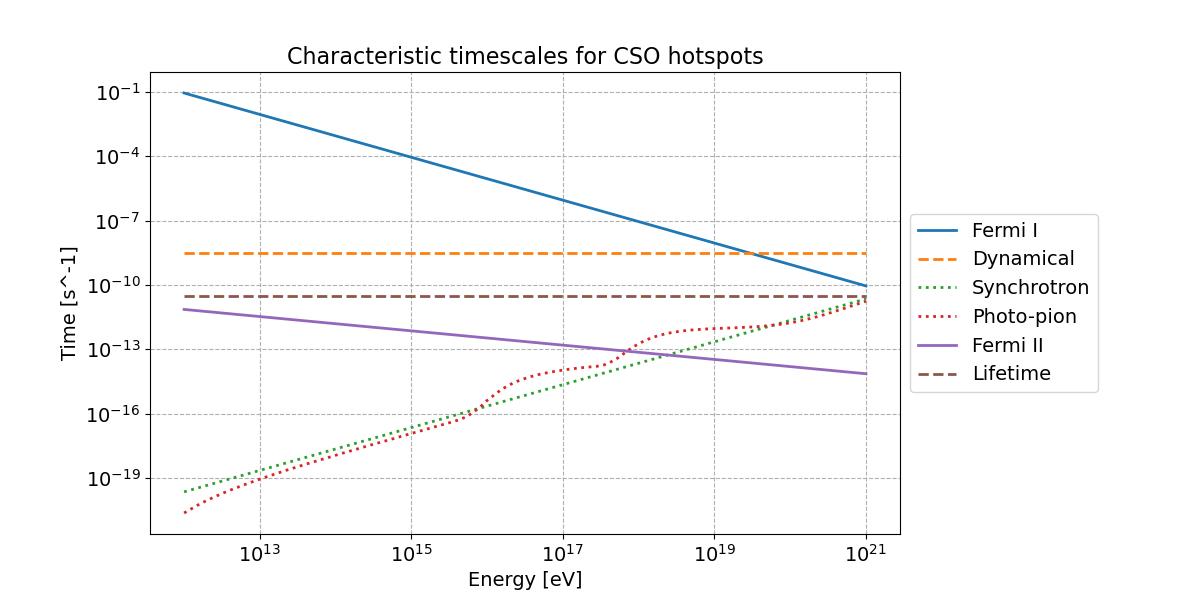
\includegraphics[width=0.8\textwidth]{C:/Users/henri/OneDrive/Documents/NTNU/Semester 10/Masteroppgave/Plots/Time_scales.png}
    \caption{Characteristic timescales for the CSO. Processes included is synchrotron losses and photopion losses. The timescales are calculated for a spherical size of $R_{\text{lobe}} = 2 pc$ and a magnetic field strength of $B = 10^{-2} G$. The photon field is based on the parameters in table \ref{tab:SED_params}.}
    \label{fig:timescales}
\end{figure}
The timescales show us that high-energy protons can, and in any case will, under the right conditions, accelerate up to energies of $<10^{20}$ eV. This limit is capped by the dynamical size of the emitting region and, of course, the magnetic field strength. The timescales also show us that the acceleration is dominated by synchrotron losses and photopion losses, and due to their small value, one would need to consider pair-pair losses as well, which is not done in this analysis. The lack of photopion loss dominance is a good sign for proton acceleration since it has been a limiting factor in other studies such as \cite{peretti2023diffusive}, where one has a higher luminosity object with processes happening even closer to the central engine. One can confirm the lack of photopion by comparing it to the work of \cite{TAKAMI2011749}, which considered a young radio AGN with much bigger lobe sizes and much higher luminosity. In this case, the photopion losses are much higher than the synchrotron losses, and the acceleration is limited by the photopion losses. But one will note that \cite{TAKAMI2011749} did not consider the lifetime of the system, that is to say, the duration for which a CSO could maintain the shock structure that allows for acceleration, which I believe would severely limit the acceleration. The lack of photopion interaction will also be a limiting factor for neutrino production, something that will be discussed in the following sections.


\subsection*{Acceleration}
From the above timescales, one can see that the maximum energy that can be obtained from the system via first-order Fermi acceleration is huge and significantly larger compared to second-order acceleration. For CSOs to remain candidates, it is clear that only first-order acceleration is possible, and therefore one will only consider this. One can justify that first-order acceleration happens in the hot spot due to the expansion of the lobes into the ambient medium. From radio observations, one has measured mildly relativistic expansion of the lobes, and with this comes naturally a shock boundary between the expanding hot spot and the ambient medium. This shock boundary produces a natural place for acceleration, and due to the compactness of CSOs, the downstream magnetic field is strong enough to allow for efficient acceleration. One can view the theoretical schematic of the shock in figure \ref{fig:CSO_shock}.

Second-order Fermi acceleration is not efficient in the CSO, which was to be expected. The acceleration is limited by the small size of the system, the low magnetic field strength, the too-high proton density, which leads to a low Alfvén wave speed, and more. One would need a substantial decrease in the diffusive acceleration timescale for second-order acceleration to be efficient. This is not the case in the CSO, and one can therefore conclude that the acceleration is dominated by first-order acceleration.

\begin{figure}
    \centering
    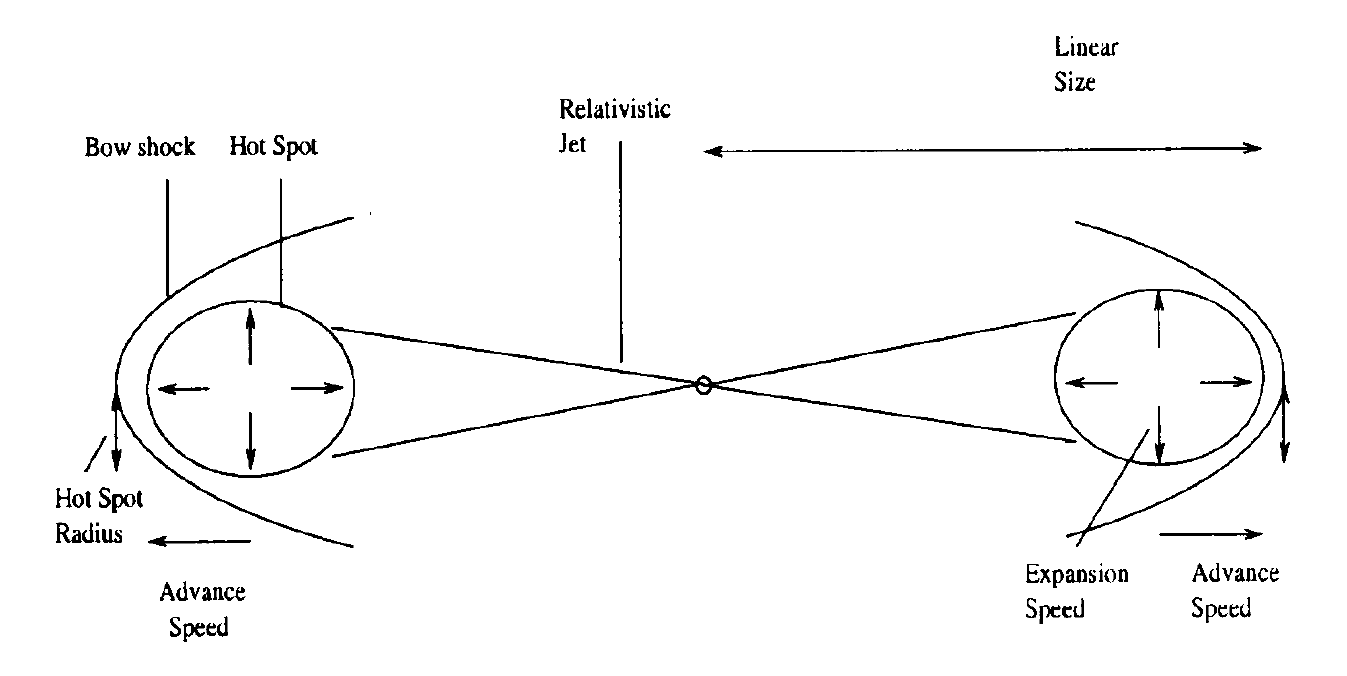
\includegraphics[width=0.5\textwidth]{C:/Users/henri/OneDrive/Documents/NTNU/Semester 10/Masteroppgave/Plots/hot_spot_expansion.png}
    \caption{Schematic of the shock in the CSO. The shock is created by the expansion of the lobes into the ambient medium through jet pressure. Image taken from \cite{Perucho_2002}}
    \label{fig:CSO_shock}
\end{figure}



\subsection{Composition/Mass Loading}
A big problem in determining the viability of UHECRs and neutrino sources is the problem of ion density and composition. The available data obtained through radio measurements or other wavelengths are usually attributed to electrons.

\subsubsection{Stellar Mass Loading}
A mechanism for the deceleration of the jet in both CSO $2.0$ and $2.1$ stages is mass loading. That being the jet encountering various densities that supply an increase of mass to the jet, slowing it down sufficiently. In \cite{sullivan2024smallscale}, they find that the jet needs a mass loading rate of $0.2 M_{\odot} \text{yr}^{-1}$ for $1000$ years in order to decelerate the jet sufficiently to explain the observed CSO $2.1$ lifetimes. This loading rate can allow us to make simple estimates of the ion density that ends up in the lobes and that may experience acceleration.

For a given mass loading rate, one can assume an initial mass composition. By assuming that the mass loading is caused by stellar objects caught by the expanding jet, one can make some estimations. These objects will have a composition similar to the solar composition. The solar composition is $74\%$ hydrogen, $24\%$ helium, and $2\%$ other elements. With this density, one can then estimate the number density of ions in the lobes assuming all mass loading ends up in the lobes via the following formula:

\begin{equation}
    n_{\text{ions}} = \frac{0.2 M_{\odot}\times 1000 \text{yr}}{\frac{4}{3} \pi R_{\text{lobe}}^3 (74\%m_p+24\%m_{\text{helium}}+2\%m_{\text{heavier ions}})}
\end{equation}

Setting $R = 10$ pc, a not unreasonable number for CSO 2.1, we get the number density of ions to be $n_{\text{ions}} = 2.9  \text{cm}^{-3}$. This is not an unreasonably high number for the number density, and it is possible that the ion density is higher than this with part of the jet energy being carried by ions. From this estimate, one also receives the metallicity of the lobes, which is $Z = 0.02$, which is the solar metallicity. This as well is not an unreasonable number but is based on the assumption that the mass loading is caused by stellar objects.

\cite{sullivan2024smallscale} find that the number of stars needed for the...

\subsubsection{Metallicity}
The metallicity of the lobes is also an unknown quantity.

\subsection{Emissivity of the System}
Based on the magnetic field strength, one can estimate the possible maximum energy achieved by a proton. In addition to this, one can estimate the number density of protons in the system through the mass loading rate and a composition by assuming it to be equal to that of solar masses. One also has the density of CSO sources to which this process is happening. With all this information and given a few assumptions on the energy spectra of the protons, one can estimate the emissivity of UHECRs from these sources.

The energy spectrum of protons undergoing first-order acceleration is usually a power law, but commonly one uses a broken power law to describe the spectrum. The spectrum of the number of protons per unit energy is given by:

\begin{equation}
    \label{eq:proton_spectrum}
    N(\gamma) = \begin{cases}
    N_0 \gamma^{-\alpha} & \gamma < \gamma_{\text{break}} \\
    N_0 \gamma_{\text{break}}\gamma^{-\alpha-1} & \gamma > \gamma_{\text{break}}
    \end{cases}
\end{equation}

By arguing that the number of ions in the lobe is equal to the total mass loaded into the lobe, $V_{\text{lobe}} n_{\text{Ion}} = \int_{\gamma_{\text{min}}}^{\gamma_{\text{max}}} N(\gamma) d\gamma$, one can normalize the spectrum. In addition to this, one can separate the number of ions into those of different species by multiplying with the percentage of the mass that is of that species. With this, one can estimate the internal energy of any desired species in the lobe. $\gamma_{\text{max}}$ can then be estimated based on the maximum energy of the particular species. The total internal energy of any species in the lobe can then be calculated as,

\begin{equation}
    U_{\text{Ion}} = m_p c^2 \int_{\gamma_{\text{min}}}^{\gamma_{\text{max}}} \gamma N(\gamma)d\gamma
\end{equation}

By assuming that all internal energy is converted to UHECRs and radiated away at a constant rate, one can estimate the luminosity of cosmic rays as $L_{\text{species}} = U_{\text{species}}/t_{\text{life}}$. One can separate the internal energy stored in all ions to those of the most energetic, that will become UHECRs by calculating the separate internal energy for UHECRs. That is to say, only ions with energy larger than $\gamma > 10^{10}$. By using our estimate of the density of CSO 2.0s at $10^{-5} \text{Mpc}^{-3}$, $\gamma_{\text{max}} = 3 \times 10^{19} \times Z$ and $\gamma_{\text{min}} = 3$, one can estimate the emissivity of UHECRs per species as $Q_{\text{UHECR}} = L_{\text{species}} n_{\text{CSO}}$.

The results of the calculations can be seen in table \ref{tab:emissivity_mass_load}.


 \begin{table}[h!]
    \centering
    \begin{tabular}{|c|c|c|c|}
    \hline
    \textbf{Variable} & \textbf{Protons} & \textbf{Helium} & \textbf{Heavier Ions} \\
    \hline
    \textbf{$u$ (erg cm$^{-3}$)} & \(8.284 \times 10^{-12}\) & \(1.075 \times 10^{-11}\) & \(6.045 \times 10^{-12}\) \\
    \hline
    \textbf{L (erg s$^{-1}$)} & \(1.020 \times 10^{48}\) & \(1.323 \times 10^{48}\) & \(7.440 \times 10^{47}\) \\
    \hline
    \textbf{$\epsilon$ (erg Mpc$^{-3}$ yr$^{-1}$)} & \(3.858 \times 10^{50}\) & \(5.005 \times 10^{50}\) & \(2.815 \times 10^{50}\) \\
    \hline
    \textbf{$u_{\text{UHECRs}}$ (erg cm$^{-3}$ )} & \(4.692 \times 10^{-29}\) & \(6.087 \times 10^{-29}\) & \(3.424 \times 10^{-29}\) \\
    \hline
    \textbf{$L_{\text{UHECRs}}$ (erg s$^{-1}$)} & \(5.774 \times 10^{30}\) & \(7.491 \times 10^{30}\) & \(4.214 \times 10^{30}\) \\
    \hline
    \textbf{$\epsilon_{\text{UHECRs}}$  (erg Mpc$^{-3}$ yr$^{-1}$)} & \(2.185 \times 10^{33}\) & \(2.835 \times 10^{33}\) & \(1.595 \times 10^{33}\) \\
    \hline
    \end{tabular}
    \caption{Mass Loading and Extra-Galactic Results for Different Species}
    \label{tab:emissivity_mass_load}
    \end{table}
 


\subsection{Neutrino Emissivity}

\newpage
\chapter{Emissivity of Particles}
\label{sec:emissivity_sec}

A big problem in determining the viability of CSOs as UHECRs and neutrino sources is the problem of ion density and composition where the available data obtained through radio measurements or other wavelengths are attributed to electrons. Therefore, we need to investigate the ion density and composition of the emitting body. In this chapter we will outline an estimate of the ion density and composition based on jet propagation into the ambient medium,  make an estimate of the emissivity of UHECRs from the hotspots of CSOs, and lastly estimate the neutrino emissivity from the same sources.


\section{Ion density and composition}
The fraction of observed CSO $2.0,2.1$, and $2.2$ suggest that the deceleration phase between $2.0$ and $2.2$ happens quite rapidly. Given the lifetime of CSOs is on the order of $10^4$ years, the deceleration phase happens on a characteristic timescale of $10^3$ years. This is a very short timescale, and in \cite{sullivan2024smallscale} they propse a mechanism for the deceleration of the jet in both CSO $2.0$ and $2.1$ stages, which is mass loading. Mass loading is the process of the jet encountering various densities that supply an increase of mass to the jet, slowing it down sufficiently. In \cite{sullivan2024smallscale}, they find a relation that relates the deceleration time to lobe parameters based on a kinetic model, and is given as

\begin{equation}
    t \approx 1000\text{yr}\times \left(\frac{r_{b}}{10  \text{pc}}\right)^{-2} \left(\frac{M_p}{1 M_{\odot}}\right) \left(\frac{c_s }{250 \text{km/s}}\right)^{-1} \left(\frac{\rho_a}{10^{-24}\text{g cm}^{-3}}\right)^{-1}
\end{equation}

The example quoted in \cite{sullivan2024smallscale} takes a $1 M\odot$ lobe with a decleration timescale of $1000$ years and through conservation of momentum they find a required mass loading of $0.2 M_{\odot} \text{yr}^{-1}$. This loading rate can allow us to make simple estimates of the ion density that ends up in the lobes and that may experience acceleration. If the mass loading was caused by mass entrainment of the ambient medium, one can estimate the density that would suffice and in \cite{sullivan2024smallscale} setting $r=10$pc and $c_s = 250$km$/$s they find that an ambient density of $8\times 10^{-25} \text{g cm}^{-3}$ is needed to decelerate the jet. This density is similar in magnitude as the density found in elliptical galaxies cores according to \cite{Capelo_2010}. 

%The density calculated seems very low, but if one assumes an equal amount of protons and electron in the jet the intial mass density of the sphere would be $1.6\times 10^{-26}$ g cm$^{-3}$, meaning that the mass loading would 


Other sources of mass entrainment instead of the ambient density could be stellar mass loading, where the jet intercepts stellar objects. With this method we can estimate species composition as well which is less clear with ambient mass loading. For the following discussion, we will assume that the mass loading is caused by stellar objects.    
 By assuming that the mass loading is caused by stellar objects caught by the expanding jet, we can make some estimations. These objects will have a composition similar to the solar composition. The solar composition by mass is $74\%$ hydrogen, $24\%$ helium, and $2\%$ other elements. We can then estimate the number density of ions in the lobes assuming all mass loading ends up in the lobes via the following formula:

\begin{equation}
    n_{\text{ions}} = \frac{\dot{M} \times t_{l} }{\frac{4}{3} \pi R_{\text{lobe}}^3 (74\%m_p+24\%m_{\text{helium}}+2\%m_{\text{heavier ions}})}
\end{equation}

Setting $R = 10$ pc, $\dot{M} = 0.2 M\odot /$year, and $t_{l} = 1000$years we get the number density of ions to be $n_{\text{ions}} \approx 0.9  \text{cm}^{-3}$. This is a number density approximately equal in magnitude than that of the lowest density gas in the interestellar medium. We also receive the metallicity of the lobes, of $2\%$, which is the solar metallicity. The metallicity is not an unreasonable number but is purley based on the assumption that the mass loading is caused by stellar objects. One important assumption is that the stellar mass loading is in the form of gas that distributes itself over the lobe. A more realistic model of mass entrainment would need to investigate the affect the jet can have one the star. Our result here is with the intent of estimating a type of composition, and the number density of ions in the lobe. 

 

%\cite{sullivan2024smallscale} find that the number of stars needed for the...


\section{UHECRs Emissivity}
\label{sec:emissivity_mass_load}
In the previous sections we have estimate the possible maximum energy achieved by a proton, the number density of CSOs, and lastly the number density and composition of ions due to mass loading. With this information and given a few assumptions on the energy spectra of the protons, we can estimate the emissivity of UHECRs from these sources.

The energy spectrum of protons undergoing first-order acceleration is usually a power law with spectral index $\alpha = 2$, but in order to incorporate energy losses one commenly use a broken power law to describe the spectrum, and a harder spectral index. The broken power law spectrum of the number of protons per unit energy is given by:

\begin{equation}
    \label{eq:proton_spectrum}
    N(\gamma) = \begin{cases}
    N_0 \gamma^{-\alpha} & \gamma < \gamma_{\text{break}} \\
    N_0 \gamma_{\text{break}}\gamma^{-\alpha-1} & \gamma > \gamma_{\text{break}}
    \end{cases}
\end{equation}

By arguing that the number of ions in the lobe is equal to the total mass loaded into the lobe, $V_{\text{lobe}} n_{\text{Ion}} = \int_{\gamma_{\text{min}}}^{\gamma_{\text{max}}} N(\gamma) d\gamma$, we can normalize the spectrum.  We can separate the number of ions into those of different species by multiplying with the percentage of the mass that is of that species. With this, we can estimate the internal energy of any desired species in the lobe. $\gamma_{\text{max}}$ is estimated based on the maximum energy of the particular species. The total internal energy of any species in the lobe can then be calculated as,

\begin{equation}
    U_{\text{I}} = m_i c^2 \int_{\gamma_{\text{min}}}^{\gamma_{\text{max}}} \gamma N(\gamma)d\gamma
\end{equation}

By assuming that all internal energy is converted to UHECRs and radiated away at a constant rate, we can estimate the luminosity of cosmic rays as $L_{\text{species}} = U_{\text{species}}/t_{\text{life}}$. In order to calculate the specific luminosity of UHECRs we separate the internal energy stored in all ions to those of the most energetic by calculating the separate internal energy for UHECRs. That is to say, only ions with energy larger than $\gamma > 10^{10}$. Using our estimate of the density of CSO $2.0$s at $10^{-5} \text{Mpc}^{-3}$, $\gamma_{\text{max}} = \frac{3 \times 10^{19} \times Z}{m_p c^2}$ and $\gamma_{\text{min}} = 1$,$\alpha =2.47$, $\gamma_{\text{break}}= 10^6$ , we can estimate the emissivity of UHECRs per species as $Q_{\text{UHECR}} = L_{\text{species}} n_{\text{CSO}}$. The value of $\alpha$ and $\gamma_{\text{break}}$ are derived by estimating that the energy loss of protons increases the original spectral index by $0.47$ and the break energy is caused by less efficient acceleration at higher energies.

The results of the calculations can be seen in table \ref{tab:emissivity_mass_load}.

\begin{table}[H]
    \centering
    \begin{tabular}{|c|c|c|c|}
    \hline
    \textbf{Variable} & \textbf{Protons} & \textbf{Helium} & \textbf{Heavier Ions} \\
    \hline
    \textbf{$u$ (erg cm$^{-3}$)} & \(1.9 \times 10^{-12}\) & \(2.5 \times 10^{-12}\) & \(1.4 \times 10^{-12}\) \\
    \hline
    \textbf{L (erg s$^{-1}$)} & \(2.3 \times 10^{47}\) & \(3.0 \times 10^{47}\) & \(1.7 \times 10^{47}\) \\
    \hline
    \textbf{$\epsilon$ (erg Mpc$^{-3}$ yr$^{-1}$)} & \(8.8 \times 10^{49}\) & \(1.1 \times 10^{50}\) & \(6.4 \times 10^{49}\) \\
    \hline
    \textbf{$u_{\text{UHECRs}}$ (erg cm$^{-3}$)} & \(9.6 \times 10^{-20}\) & \(1.2\times 10^{-19}\) & \(7.0 \times 10^{-20}\) \\
    \hline
    \textbf{$L_{\text{UHECRs}}$ (erg s$^{-1}$)} & \(1.2 \times 10^{40}\) & \(1.5 \times 10^{40}\) & \(8.6 \times 10^{39}\) \\
    \hline
    \textbf{$\epsilon_{\text{UHECRs}}$  (erg Mpc$^{-3}$ yr$^{-1}$)} & \(4.5 \times 10^{42}\) & \(5.8 \times 10^{42}\) & \(3.3 \times 10^{42}\) \\
    \hline
    \end{tabular}
    \caption{Mass Loading and Extra-Galactic Results for Different Species}
    \label{tab:emissivity_mass_load}
\end{table}
 
The values of the calculation give reasonable values for the emissivity of UHECRs, but not reasonable values for the luminosity of all protons. The luminosity of the protons is a factor $100$ higher than the most powerful jet in figure \ref{fig:jet_power} which makes this unphysical. The average ion density is very low,  but this is a consequence of very efficient mass shedding via CR acceleration. One preformed the same test by equating the ion energy density to the magnetic field density, and the results can be seen in the Appendix. 
%And this is still under the assumption of a very low estimate for the ion density. In addition, we check for a different scenario in which we equates the ion energy density to the magnetic field density. Again the magnetic field density is given as $u_B = \frac{B^2 }{ 8 \pi} = 3.98 \times 10^{-6}$ for a magnetic field of $B = 10^{-2}$ G. The results of this assumption can be seen in table \ref{tab:emissivity_mass_load_B}. 




%Here we has a overshot the emissivity of UHECRs when comparing it to the measured emissivity discussed in section \ref{sec:emmisivity}, with the emissivity of UHECRs being of the order of $5\times 10^{46}$ erg Mpc$^{-3}$ yr$^{-1}$. These values are incedibly high and are unreasonable to this extent that one does not see this type of local emissivity. With this argument it becomes clearer that equating the ion density to the magnetic field density might not be necessary. The result in table \ref{tab:emissivity_mass_load_B} is contingent on the emission region since a bigger emission region will allow for higher number of ions, but the table in \ref{tab:emissivity_mass_load} is only contingent on the mass loaded by stellar mass loading. The emissivity of UHECRs from the stellar mass loading argument would be approximately $2\%$ of the total emissivity. This is a reasonable number, that could be higher if paramters such as ion density, CSO number density, or mangetic field strength are higher.

Both these results overshoot their total comsic ray luminosity since the CR luminosity is higher than even the highest jet power. This makes the result unreasonable, and one should almost certainly tweek our paramters. It is clear that if all entrained mass, stellar or from the ambient density ends up in the lobes, and is accelerated the luminosity will be too high. We argue that not all mass ends up being accelerated. In order for the UHECRs luminosity to be of significant values and keeping the luminosity of CR at a reasonable value one should consider two things. Firstly that not all mass is accelerated and escapes. The consequence of this is that most entrained mass will be cold protons that follow the jet, and do not escpae the system in our given time frame. Secondly one would like to consider a softer spectrum of protons, which will increase the relative emission of UHECRs. If this is reasonable is not yet clear but allows for comparison. We run the model on this biased choice of parameters. We  assume that only $0.01\%$ of the mass loaded into the lobe is accelerated, and only a single power law spectrum for our protons with $\alpha = 2.47$. The result of this configuration can be seen in table \ref{tab:emissivity_mass_load_1}.
\begin{table}[H]
    \centering
    \begin{tabular}{|c|c|c|c|}
    \hline
    \textbf{Variable} & \textbf{Protons} & \textbf{Helium} & \textbf{Heavier Ions} \\
    \hline
    \textbf{$u$ (erg cm$^{-3}$)} & \(4.8 \times 10^{-4}\) & \(6.2 \times 10^{-4}\) & \(3.5 \times 10^{-4}\) \\
    \hline
    \textbf{L (erg s$^{-1}$)} & \(2.3 \times 10^{44}\) & \(3.0 \times 10^{44}\) & \(1.7 \times 10^{44}\) \\
    \hline
    \textbf{$\epsilon$ (erg Mpc$^{-3}$ yr$^{-1}$)} & \(8.9 \times 10^{46}\) & \(1.1 \times 10^{47}\) & \(6.5 \times 10^{46}\) \\
    \hline
    \textbf{$u_{\text{UHECRs}}$ (erg cm$^{-3}$)} & \(2.7 \times 10^{-19}\) & \(4.2 \times 10^{-19}\) & \(2.3 \times 10^{-19}\) \\
    \hline
    \textbf{$L_{\text{UHECRs}}$ (erg s$^{-1}$)} & \(3.3 \times 10^{40}\) & \(5.1 \times 10^{40}\) & \(2.9 \times 10^{40}\) \\
    \hline
    \textbf{$\epsilon_{\text{UHECRs}}$  (erg Mpc$^{-3}$ yr$^{-1}$)} & \(1.3 \times 10^{43}\) & \(1.9 \times 10^{43}\) & \(1.1 \times 10^{43}\) \\
    \hline
    \end{tabular}
    \caption{Emissivity of CR and UHECRs for different species with a single powerlaw spectrum and a low percent of mass loaded into the lobe expericening acceleration.}
    \label{tab:emissivity_mass_load_1}
\end{table}


Our results have succeeded in lowering the luminosity of CR with an added cost of significantly increasing the energy density of ions in the lobes, due to the cold protons introduced. The energy density of our magnetic field in this scenario is of the order $10^{-6}$ meaning that the remaining energy density of cold protons is quite high. The comparisson between the two cases hints at an equilibrium where the ion density of ions does not get too high due to the radiative efficiency of the lobe of dispelling them. This is hypothetical, but with the fact that the lobe would most likely entrain mass, a good question is what happens to those ions.
The observation we derive from this is that the lobes of CSOs have a viable source of ions which can be accelerated to CR. The additonal observation is that with this model with parameters taken from \cite{sullivan2024smallscale} the non acceleration of entrained mass will likely lead to a high energy density of ions in the lobes. 

One assumed a stellar composition of the mass loaded into the lobe in order to study the distribution of emissivity across species. The results show that the species distributed emissivities are of equal order magnetiude with helium ions carrying the most energy out. Therefore, if the compositon of UHECRs in the hotspots include helium ions, and heavier ions it is reasonable to assume that they will carry a substantial amount of the energy out of the system. 


 

%\subsection{Motivation for luminosity of UHECRs}
%In order to look for luminosity of UHECRs from the lobes, we argue that the energy budget of the jet can reveal some interesting dynamics.  We argue that in the system of the lobe expansion into the ambient medium the energy calculation should be a zero if one includes all sources of loss. The equation for the resulting power budget in the jet can be written as 





\section{Neutrino Emissivity}
Lastly, we might like to look for neutrinos from the same sources as the UHECRs. We aim here to calculate the expected fraction of neutrinos produced via the photopion effect in the hotspots of the CSO from the escaping protons. From our estimate of the photopion timescale in the previous sections, we can estimate the resulting flux of neutrinos as a relation to the escaping protons. The methodology is taken from \cite{Oikonomou_2019}.
Given the number of protons escaping the system, one can estimate the number of neutrinos produced as

\begin{equation}
\epsilon_{\nu}^2 \frac{dN_{\nu}}{d\epsilon_{\nu}} = \frac{1}{4} f_{p\gamma}f_{\pi, \text{cool}} f_{\mu,\text{cool}}\epsilon_p^2 \frac{dN_{p}}{d\epsilon_{p}}
\end{equation}

where $f_{p\gamma}$ is the fraction of lost protons that undergo the photopion interaction defined as, $f_{p\gamma} = t_{p\gamma}/t_{\text{cool}}$, $f_{\pi, \text{cool}}$ and $f_{\mu, \text{cool}}$ are suppression factors that take into account energy loss from pions and muons respectively defined as $f_{\pi, \text{cool}} = 1-\exp{(-t_{\pi,\text{cool}}/t_{\pi, \text{dec}})}$. Where $t_{\pi,\text{cool}} = t_{\pi, \text{syn}} + t_{\text{dyn}}$, $t_{\pi, \text{dec}} = \gamma_{\pi}\tau_{\pi}$ with $\tau_{\pi} = 2.6\times 10^{-8}$ and $\tau_{\mu} = 2.2\times 10^{-6}$.

One is not intending on finding the specific neutrino flux since the prefactor will illuminate the desired trend of the system. The energy-dependent prefactor can be seen in figure \ref{fig:neutrino_flux_prefactor}.

\begin{figure}
    \centering
    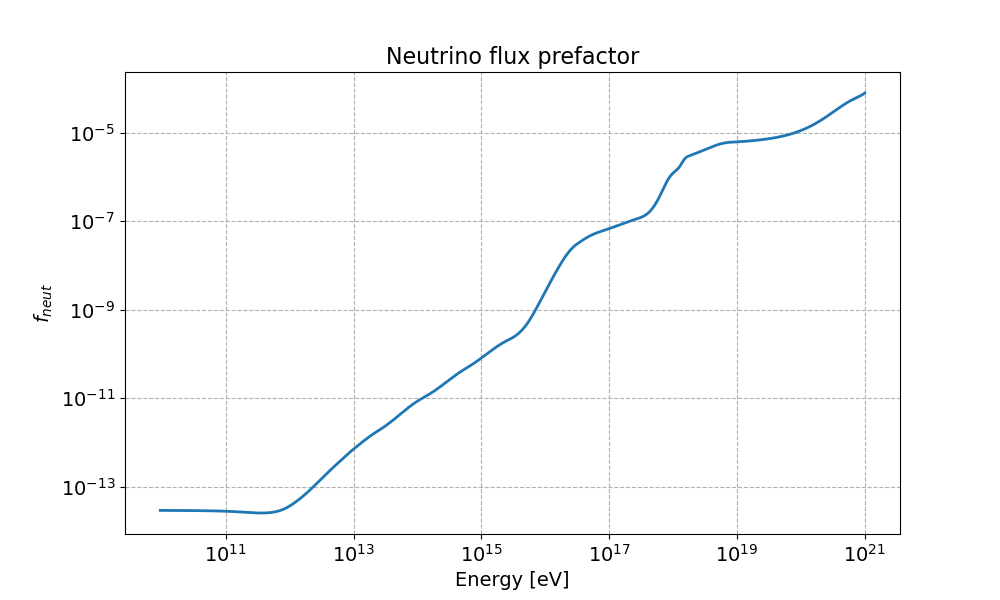
\includegraphics[width=0.8\textwidth]{C:/Users/henri/OneDrive/Documents/NTNU/Semester 10/Masteroppgave/Plots/Neutrino_flux_prefactor.png}
    \caption{Energy-dependent prefactor for the neutrino flux as a function proton losses. The prefactor is calculated for CSO hotspots, and the photopion effect from figure \ref{fig:timescales}.}
\label{fig:neutrino_flux_prefactor}
\end{figure}

Here one sees that the maximum ratio of proton flux to neutrino flux is around $10^{-5}$, a significantly low number. Due to the fact that the emissivity of UHECRs and neutrinos are of the same order of magnitude, one can conclude that the neutrino flux from the CSO hotspots is not significant. This is not surprising since the photopion losses are not dominating the acceleration. But there is still a case to be made for the CSO core, which is not covered here.


\newpage
\chapter{Discussion/Future work}
%\section{Discussion}

The methods used in this thesis have been able to show that CSOs hotspots are viable sources of UHECRs and not neutrinoes. The results are not as robust as we would like due to the low level of data found on CSOsand the unconstrained parameters used in chapter \ref{sec:emissivity_sec}, but we argue that they are indicative of the potential of CSOs. Given the new criteria for CSOs and the semi-novel idea of them being transient sources the possibility of them contributing to the local UHECR 
emissivity has increased. 

From the initial distribution of the known CSOs seen in chapter \ref{sec:CSO} it became clear that we are observing the most luminous part of their luminosity function. We have not derived a relation between the radio luminosity of the lobes and their luminosity of CR, but with more data this could be possible. The increase of detection of this subclass of AGN can be beneficial for the field of comsic ray origin, and the study of the most energetic particles in the universe. 

Given that CSOs, or at least CSO 2.0 and 2.1, can accelerate ions to the highest energies, we still have a problem of detection. According to the modern view of particle propagation through the interstellar medium (ISM) and the galactic medium (GM), particles such as protons and heavier elements will get scattered and deflected by the underlying magnetic field filling the ISM and GM. Therefore, the travel time of a photon and UHECRs from the same source will differ significantly.
As explained in \cite{Murase_2008} the average delay time for UHECRs is given by

\begin{equation}
    \bar{t}_d \approx \frac{D \theta^2 d}{4c} \simeq 10^5 \, \text{yrs} \left( \frac{D^2_{100 \, \text{Mpc}} B^2_{\text{IG},-9} \lambda_{\text{Mpc}}} {E_{20}^2}\right)
\end{equation}

Where $D$ is the distance to the source in units of Mpc, $E_{20}$ is the energy of the UHECR in units of $10^{20}$ eV, $B_{\text{IG}}$ is the strength of the intergalactic magnetic field in units of $10^{-9}$ G, and $\lambda$ is the coherence length of the magnetic field in Mpc. With characteristic values also obtained in \cite{Murase_2008} of $D = 50$ Mpc, $B_{\text{IG}} = 10^{-9}$ G, and $\lambda = 1$ Mpc, one sees that the average delay time is of the order of the lifetime of a CSO. 

This poses a challenge when groups such as the auger group try to retrace measured UHECRs to a CSO. The challenge is that one will no longer find that CSO. CSOs, being transient events with a lifetime of only a maximum of $(10^4)$ years, will possibly have disappeared from the night sky when their emitted UHECRs arrive at Earth. Therefore, the detection of UHECRs from CSOs could rely on the non-detection of any obvious sources when retracing the UHECRs. In addition to this, one could hope that the CSO will have some relic signature in the form of a radio-emitting region that has not yet disappeared, but this is no guarantee. The point of this passage is to highlight the possible difficulty in detecting UHECRs from CSOs and that the co-detection of both UHECRs and subsequent photons from the same source could be a rare event.

The SED modeling seen in chapter \ref{sec:photon_fields} have similarties of different groups who have done the same thing. In \cite{bronzini2024investigating} and in \cite{Ostorero_2010} the biggest difference comes in the contribution of IC and SSC emission. We explain this difference due to the fact that they did entire jet, lobe and core modeling of the emitting galaxy core, while we only focused on the hotspot. Our IC and SSC is the reuslt of only the electrons in the hotspot. We have added a factor 2 to their IC and SSC emission to account for two hotspots, but this is a very rough estimate. In future work we would like to incorporate the entire jet, and begin using observed data to constrain our model. For the moment the spectral fields created served their purpose and from small testing it is clear that an increase in IC and SSC emission would not change the photopion interaction significantly. The potential gain of using observational data to minimize the parameter space is clear. It would allow us to calculate upper limits on electron parameters, which one could expect protons to follow as well. As we have seen as well, the amount of power supplied in X-ray can also be used to constrain the amount of power in the jet further constraining the parameter space. Lastly the accretion rate can be constrained which would allow for better modeling of the interaction between the jet and the accretion disk.

The parameter estimation done in chapter \ref{sec:CSO_UHECR} showed that the different methods of determining size and mangetic field strength can vary quite largly between each other. This is a problem that is rooted in our data collection and the lack of observational data collected makes it hard for us to see any errortrends. The results still give us good estimations of the parameters, and have not limited the continued work in the project, but a bigger dataset with more clear constraints would be benificial. The magnetic field value of $0.01-1$ G is in line with other observed values of GHz peaked galaxies as measured in \cite{cheng2023highfrequency} which measured between $0.01 -0.05$ G. These values are more on the lower side, and shows why we chose to use conservative values further in our analysis.  

The radius estimates of our hotspots fall in line with what others have measrued as well but for GHz peaked galaxies. \cite{Perucho_2002} estiamtes a realtion between hotspot size and linear size of the source, and the order of magnetidue for his hotspots are $2-11$pc which is in line with our estimates. The same relation between linear size and hotspots can not be seen, but there is as mentioned before a large scatter in the data. The scatter is due to us not including viewing angle in our estimate of the hotspot, due to our assumption that it is spherical. The work from \cite{Perucho_2002} also show the same type of scatter that we see, where the linear size relation estimates on average a factor $10$ larger than the hotspot size. This has proven not to be a problem for our work, since when calculation the jet power of our sources, which is the only place we use this linear size relation the desired size is no longer only the hotspot, but the entire lobe. For future work, as always more data would be appreciated, and possible time variability estimates of the hotspots. 


The jet power which is affected by the estimation of the size and magnetic field values gave large values for the jet but they are within other measruements as made by \cite{W_jtowicz_2020} and are possible as written in \cite{readhead2023compact}. Therefore we can be farily confident in our fidnings. The reason for the X-ray inferred jet power being substantially lower, might be due to bad paramter estimation of the prefactor. In \cite{readhead2023compact} they show that the jetpower is related to the accretion rate via a factor $k \in (0.2-2)$ instead of $\eta_j \in (0.001-0.1)$ as we have used and is found in \cite{W_jtowicz_2020}. Both values estiamte the same thing which is accretion efficiency, and the values in \cite{readhead2023compact} are theoretical based on the rotation of the SMBH. Therefore we have more confidence using infeered efficiency as done in \cite{W_jtowicz_2020} but that the discrepancy between the two jet powers could be due to underestimation of the accretion efficiency. The other side of the coin is that we might have overestimated the minimum jet power, due to applying a the magnetic field measruements to the entire lobe. The calculation we have done are self consistent, but allowing for different energy densities in different parts of the jet, which does seems reasonable could yield a better estimation for the minimum jet power. Future work in this area would hopefully include some better constraint on the jet power, where one could do as explaine in \cite{Wykes_2013} of using enthalphy measruements or more direct measruements of the accretion disk, circumventing the need for x-ray to accretion disk power relations. Our result agree given our large errorbars, but the large errobars are indicative of the need for more and better constrained data on the individual sources. One parameter that might be worth measuring would be the shock speed or expansion speed as it is called. This would allow us to test other parameters in the minimum jet model and reach a more robust conclusion. 

The reuslt of Jet power put into future work can yield interesting result. Kinetic models such as used in \cite{sullivan2024smallscale} assume that all jet power is being counterbalanced with the ram pressure by the ambient medium, and that radiation losses are negligible. This assumption usually lead to the need for high ambient density or stellar mass loading as we have explored. But as seen in our result for the emissivity, a substantial sink of energy could be the acceleration of protons, and estimating a proper energy budget for the jet and its losses could, and i preface could lead to a need for more energy loss than is observed via radiation.

From our timescale analysis it became apparent that there are no large energy losses during the protons acceleration. The paramter that determined the cutoff was the size of our emitting system, and given that our model assumed a value on the lower end of our range $R = 2$ pc, it leads to the maximum possible energy achieved by protons is of the order $10^20$ eV. For future work in this area, creating the relation between maximum energy and size of the system good be interesting when calculating the contribution of CSOs to the spectra of UHECRs. With this hypothetical relation one can superimpose it on an luminosity function of CSOs and be able to more accurately estimate the contribution of CSOs to the UHECR emissivity, and its resulting spectrum. 

The timescale estimate also allowed us to estimate the resulting neutrino luminosity as a function of the proton luminosity, which showed that neutrinos are not very likely being produced in the hotspots of CSOs. The timescale for pion production is simply too long and the fraction of escaped protons producing neutrinos is too low. There is still areas of intereste that can produce neutrinos. In \cite{neronov2023neutrino} they discuss neutrino emission from seyfert galaxies, and in \cite{Kalashev_2023} they discuss neutrino emission from the central parsec of Blazar cores showing that the entire pciture of CSOs as neutrino produces has barley been scratched. 


Our simple analysis on mass loading and the subsequent acceleration of ions loaded into the lobe showed that there is possibly an equilirbium point between the ion density and the reuslting CR luminosity. For our results it is clear that the luminosity of protons is too high, and by adjusting our parameters we showed that the luminosity could be lowered but at the cost of a high ion energy density. This problem is not necessarly as big as one has stated since the values in which we are operating with are extremely unconstrained. The intial mass of the lobe which lead to the required mass loading are not unreasonable but not obersvationally bounded either. The result show if nothing else that the balance between cold protons and CR protons might be delicate, and the mass loading of the jet could be a key factor of introducing protons into the shocked area. The method of introducing protons via mass loading is also discuess in \cite{Wykes_2013} where they use a mass entrainment model of both ambient density and stellar loading. The result they acheive requries the particles to be heated in order to fix an imbalance of pressures as a result of mass loading. We have not moved further into such a model, but future work could include a better estimates on the effect of the mass entrainment on the lobe. 














 







\newpage
\chapter{Conclusion}
The main results of the thesis is that CSOs, more specifically CSO hotspots which are found in the jet termination area of CSO show great potential in being UHECRs sources, but not neutrino sources. 

We investigated the new list of CSO object produced by \cite{kiehlmann2023compact} and came to similar conclusion that they have sample the higher end of the luminosity function for CSOs. 

We have calculated the magnetic field of a selection of CSOs  included in the new list presented by \cite{kiehlmann2023compact}. The selection covered overlapping entries between the list compiled in \cite{kiehlmann2023compact} and a list of radio observation done by \cite{nrao1996}.  The hotspot from the overlapping sources vary from $0.01-1$ Gauss using two methods where the synchrotron self absorption method gives the highest value of magnetic field for sources that were imaged close to their turnover frequency. Mangetic equipartion estimated a magnetic field strenght between $0.01-0.1$ Gauss for most sources. The radius of our emitting region was estimated to be between $1-10$ pc for the same subsample of CSOs which coincides with previous results. Using these estimates we place the CSO hotspots in the hillas diagram showing them to be potent accelerators being able to reach energies of $10^{20}$ eV.
The minimum jet power and X-ray inferred jet power was calculated for a new subsample between \cite{kiehlmann2023compact} and \cite{W_jtowicz_2020}.  The minimu jet power of the stronges CSOs in the sample were of the order of mangnitude $10^{45}$ erg/s wheras the X-ray inferred sample measured a highest jet power of $2\times 10^{44}$ erg/s. The reuslts were reasonable and in agreement with  similar calculation found in \cite{W_jtowicz_2020}. We also calculated the X-ray emissivity of our sources using the estimated density of CSOs calculated as $1.2 \times 10^{-5}$ Mpc$^{-3}$ and the X-ray luminosity. This showed that compared to other AGNs the CSOs show a high or equivalent X-ray emissivty making them good candidates. 

Using conservative parameters calculated previously we estimated the characteristic timescales of a hypothetical proton being accelerated in the hotspot and showed that the proton would be able to reach energies of $10^{20}$ eV with the size of the system being the limiting factor. The timescales also showed that significant energloss mechanism were not present in the hotspot, making neutrino production unlikely via the photo-pion production mechanism.

Mass loading was introduced as a possible deceleration mechanism to explain the lifetimes of the different CSO 2 subclasses in previous literature. We used the mass loading as a potential source of protons to experience acceleration and showed that if all mass loading was converted to protons the Cosmic ray luminosity would be higher than the jet power of the CSOs making it unreasonable. We showed that the introduction of cold protons with a small fraction of protons being accelerated away could reduce the CR luminosity to a reasonable level, but would increase the energy density of ions making it higher than the magnetic field energy density. One concluded that the unconstrained variables in the mass loading model made it difficult to draw any conclusions, but that the model showed potential in using hotspots as UHECR sources.
\newpage
\printbibliography
\newpage
\chapter*{Appendix}
%\section{Appendix A}

\section{Appendix A1 - Catalouge of CSOs}
\begin{table}[H]
    \centering
    \caption{Catalouge of bona fide CSOs. Data taken from \cite{kiehlmann2023compact}}
    \label{tab:CSO_sources}
    \begin{tabular}{@{}ccccccccc@{}}
        \toprule
        ID & R.A. & Dec. & z & Ang\_size & Lin\_size & $\nu_t$ & $S_\nu$ & Class \\ \midrule
        J0000+4054 & 00:00:53.08 & +40:54:01.81 & nan & 124.0 & nan & 0.323 & 2.06 & nan \\
        J0003+4807 & 00:03:46.04 & +48:07:04.14 & nan & 16.2 & 0.139 & 2.123 & 0.348 & nan \\
        J0029+3456 & 00:29:14.24 & +34:56:32.25 & 0.517 & 29.1 & 0.180 & 0.8 & 2.0 & 2.1 \\
        J0111+3906 & 01:11:37.32 & +39:06:28.10 & 0.66847 & 8.0 & 0.056 & 4.0 & 1.33 & 2.0 \\
        J0119+3210 & 01:19:35.00 & +32:10:50.06 & 0.0602 & 100.0 & 0.115 & 0.4 & 4.0 & 2.2 \\
        J0131+5545 & 01:31:13.82 & +55:45:12.98 & 0.003649 & 23.0 & 0.016 & 0.657 & 0.31 & 2.2 \\
        J0132+5620 & 01:32:20.45 & +56:20:40.37 & nan & 12.2 & 0.104 & 3.42 & 0.6 & nan \\
        J0150+4017 & 01:50:19.61 & +40:17:30.02 & nan & 103.0 & 0.882 & 0.4 & 2.0 & nan \\
        J0204+0903 & 02:04:34.76 & +09:03:49.26 & nan & 33.0 & 0.282 & 1.3 & 2.0 & nan \\
        J0237+4342 & 02:37:01.21 & +43:42:04.18 & nan & 120.0 & nan & 0.3 & 0.868 & nan \\
        J0402+8241 & 04:02:12.68 & +82:41:35.13 & nan & 72.0 & 0.616 & 0.4 & 0.4 & nan \\
        J0405+3803 & 04:05:49.26 & +38:03:32.24 & 0.05505 & 42.0 & 0.044 & 0.07 & 5.5 & 2.0 \\
        J0425-1612 & 04:25:53.57 & -16:12:40.23 & nan & 99.8 & 0.854 & 0.363 & 1.449 & nan \\
        J0427+4133 & 04:27:46.05 & +41:33:01.10 & nan & 7.0 & 0.060 & 3.3 & 0.74 & nan \\
        J0440+6157 & 04:40:46.90 & +61:57:58.57 & nan & 30.0 & 0.257 & 1.7 & 0.24 & nan \\
        J0706+4647 & 07:06:48.07 & +46:47:56.45 & nan & 63.0 & 0.539 & 0.777 & 1.81 & nan \\
        J0713+4349 & 07:13:38.16 & +43:49:17.21 & 0.518 & 35.0 & 0.217 & 1.9 & 2.09 & 2.0 \\
        J0735-1735 & 07:35:45.81 & -17:35:48.50 & nan & 28.8 & 0.246 & 1.4 & 3.0 & nan \\
        J0741+2706 & 07:41:25.73 & +27:06:45.42 & 0.772139 & 26.0 & 0.193 & 1.0 & 1.05 & 2.0 \\
        J0754+5324 & 07:54:15.22 & +53:24:56.45 & nan & 26.0 & 0.223 & 1.24 & 0.634 & nan \\
        J0825+3919 & 08:25:23.68 & +39:19:45.76 & 1.21 & 70.7 & 0.591 & 0.517 & 1.77 & 2.1 \\
        J0832+1832 & 08:32:16.04 & +18:32:12.12 & 0.154 & 30.7 & 0.081 & 1.5 & 1.2 & 1 \\
        J0855+5751 & 08:55:21.36 & +57:51:44.09 & 0.025998 & 75.0 & 0.039 & 0.3 & 1.5 & 2.1 \\
        J0906+4124 & 09:06:52.80 & +41:24:30.00 & 0.0273577 & 11.1 & 0.006 & 1.5 & 0.06 & 1 \\
        J0909+1928 & 09:09:37.44 & +19:28:08.30 & 0.027843 & 14.7 & 0.008 & 6.0 & 0.12 & 1 \\
        J0943+1702 & 09:43:17.23 & +17:02:18.97 & 1.601115 & 20.4 & 0.175 & 4.0 & 0.4 & 2.0 \\
        J1011+4204 & 10:11:54.18 & +42:04:33.38 & nan & 115.0 & 0.984 & 0.424 & 1.16 & nan \\
        J1025+1022 & 10:25:44.20 & +10:22:30.00 & 0.045805 & 19.8 & 0.018 & 1.0 & 0.09 & 1 \\
        J1035+5628 & 10:35:07.04 & +56:28:46.79 & 0.46 & 38.0 & 0.221 & 1.3 & 1.87 & 2.0 \\
        J1042+2949 & 10:42:36.51 & +29:49:45.15 & nan & 45.0 & 0.385 & 0.7 & 1.0 & nan \\
        J1111+1955 & 11:11:20.07 & +19:55:36.01 & 0.299 & 15.5 & 0.068 & 1.305 & 1.1 & 2.0 \\
        J1120+1420 & 11:20:27.81 & +14:20:54.97 & 0.362 & 101.0 & 0.507 & 0.5 & 3.89 & 2.0 \\
        J1135+4258 & 11:35:55.99 & +42:58:44.65 & nan & 29.0 & 0.248 & 1.0 & 1.45 & nan \\
        J1148+5924 & 11:48:50.36 & +59:24:56.36 & 0.01075 & 54.8 & 0.012 & 6.149 & 0.573 & 1 \\
        J1158+2450 & 11:58:25.79 & +24:50:18.00 & 0.203 & 46.0 & 0.152 & 2.0 & 1.25 & 2.2 \\
        J1159+5820 & 11:59:48.77 & +58:20:20.31 & 1.27997 & 70.2 & 0.591 & 0.6 & 1.9 & 2.0 \\
        J1204+5202 & 12:04:18.61 & +52:02:17.62 & nan & 54.0 & 0.462 & 0.7 & 1.4 & nan \\

        \bottomrule
    \end{tabular}
\end{table}

\begin{table}[H]
    \centering
    \begin{tabular}{@{}ccccccccc@{}}
        \toprule
        ID & R.A. & Dec. & z & Ang\_size & Lin\_size & $\nu_t$ & $S_\nu$ & Class \\ \midrule
        J1205+2031 & 12:05:51.50 & +20:31:19.00 & 0.02378857 & 22.0 & 0.010 & 1 & 0.14 & 2.1 \\
        J1220+2916 & 12:20:06.82 & +29:16:50.72 & 0.002 & 46.8 & 0.002 & 0.074 & 0.65 & 1 \\
        J1227+3635 & 12:27:58.72 & +36:35:11.82 & 1.975 & 58.8 & 0.499 & 1.2 & 2.14 & 2.0 \\
        J1234+4753 & 12:34:13.33 & +47:53:51.24 & 0.373082 & 27.4 & 0.140 & 1.4 & 0.36 & 2.1 \\
        J1244+4048 & 12:44:49.19 & +40:48:06.15 & 0.813586 & 70.0 & 0.529 & 0.405 & 2.03 & 2.2 \\
        J1247+6723 & 12:47:33.33 & +67:23:16.45 & 0.107219 & 5.0 & 0.010 & 1.16 & 0.36 & 2.0 \\
        J1254+1856 & 12:54:33.27 & +18:56:01.93 & 0.1145 & 4.14 & 0.008 & 6.0 & 0.13 & 1 \\
        J1311+1658 & 13:11:23.82 & +16:58:44.22 & 0.081408 & 27.0 & 0.041 & 0.447 & 0.824 & 1 \\
        J1313+5458 & 13:13:37.85 & +54:58:23.91 & 0.613 & 57.0 & 0.384 & 0.555 & 1.65 & 2.2 \\
        J1326+3154 & 13:26:16.51 & +31:54:09.52 & 0.36801 & 68.0 & 0.345 & 0.5 & 7.03 & 2.2 \\
        J1335+5844 & 13:35:25.93 & +58:44:00.29 & nan & 12.9 & 0.110 & 4.9 & 0.9 & nan \\
        J1347+1217 & 13:47:33.36 & +12:17:24.24 & 0.121 & 100.0 & 0.215 & 0.4 & 8.86 & 2.2 \\
        J1400+6210 & 14:00:28.65 & +62:10:38.59 & 0.431 & 67.6 & 0.378 & 0.5 & 6.56 & 2.2 \\
        J1407+2827 & 14:07:00.40 & +28:27:14.69 & 0.077 & 11.0 & 0.016 & 4.9 & 3.0 & 2.1 \\
        J1413+1509 & 14:13:41.66 & +15:09:39.51 & nan & 15.0 & 0.128 & 2.5 & 0.47 & nan \\
        J1414+4554 & 14:14:14.85 & +45:54:48.73 & 0.186 & 30.5 & 0.094 & 0.693 & 0.396 & 2.1 \\
        J1416+3444 & 14:16:04.18 & +34:44:24 & nan & 81.0 & 0.693 & 0.7 & 2.1 & nan \\
        J1434+4236 & 14:34:27.86 & +42:36:20.06 & 0.452 & 68.3 & 0.393 & 0.074 & 1.67 & 2.2 \\
        J1440+6108 & 14:40:17.87 & +61:08:42.88 & 0.445365 & 30.0 & 0.171 & 0.4 & 0.48 & 2.1 \\
        J1443+4044 & 14:42:59.32 & +40:44:28.94 & nan & 123.4 & nan & 0.292 & 1.55 & nan \\
        J1508+3423 & 15:08:05.70 & +34:23:23.00 & 0.045565 & 280.0 & 0.247 & 0.23 & 0.25 & 2.1 \\
        J1511+0518 & 15:11:41.27 & +05:18:09.26 & 0.084 & 10.6 & 0.017 & 0.4 & 0.48 & 2.0 \\
        J1559+5924 & 15:59:01.70 & +59:24:21.84 & 0.0602 & 11.0 & 0.013 & 0.15 & 0.23 & 1 \\
        J1602+5243 & 16:02:46.38 & +52:43:58.40 & 0.105689 & 250.0 & 0.478 & 0.15 & 1.48 & 1 \\
        J1609+2641 & 16:09:13.32 & +26:41:29.04 & 0.473 & 61.3 & 0.362 & 1.1 & 5.44 & 2.1 \\
        J1645+2536 & 16:44:59.07 & +25:36:30.64 & 0.588 & 39.0 & 0.258 & 1.0 & 1.1 & 2.1 \\
        J1723-6500 & 17:23:41.03 & -65:00:36.61 & 0.01443 & 7.0 & 0.002 & 2.7 & 4.48 & 2.1 \\
        J1734+0926 & 17:34:58.38 & +09:26:58.26 & 0.735 & 12.8 & 0.093 & 2.3 & 1.22 & 2.0 \\
        J1735+5049 & 17:35:49.01 & +50:49:11.57 & 0.835 & 8.0 & 0.061 & 6.4 & 0.972 & 2.0 \\
        J1816+3457 & 18:16:23.90 & +34:57:45.75 & 0.245 & 45.5 & 0.174 & 0.44 & 0.983 & 2.1 \\
        J1826+1831 & 18:26:17.71 & +18:31:52.89 & nan & 74.0 & 0.633 & 0.308 & 1.08 & nan \\
        J1826+2708 & 18:26:32.11 & +27:08:07.95 & nan & 41.0 & 0.351 & 1.0 & 0.34 & nan \\
        J1915+6548 & 19:15:23.82 & +65:48:46.39 & 0.486 & 36.0 & 0.216 & 0.5 & 0.83 & 2.1 \\
        J1928+6815 & 19:28:20.55 & +68:14:59.27 & nan & 128.1 & nan & 0.074 & 1.04 & nan \\
        J1939-6342 & 19:39:25.02 & -63:42:45.62 & 0.183 & 42.6 & 0.130 & 1.4 & 15.0 & 2.0 \\
        J1944+5448 & 19:44:31.51 & +54:48:07.06 & 0.263 & 48.8 & 0.196 & 0.778 & 1.77 & 2.0 \\
        J1945+7055 & 19:45:53.52 & +70:55:48.73 & 0.101 & 40.6 & 0.075 & 1.8 & 0.929 & 2.2 \\
        J2022+6136 & 20:22:06.68 & +61:36:58.80 & 0.2266 & 29.0 & 0.104 & 4.086 & 2.64 & 2.1 \\
        J2203+1007 & 22:03:30.95 & +10:07:42.59 & 1.005 & 11.0 & 0.089 & 4.427 & 0.306 & 2.0 \\
        J2327+0846 & 23:27:56.70 & +08:46:44.30 & 0.02892 & 1300.0 & 0.744 & 0.09 & 1.0 & 1 \\
        J2347-1856 & 23:47:08.63 & -18:56:18.86 & nan & 33.4 & 0.186 & 1.8 & 0.66 & nan \\
        J2355+4950 & 23:55:09.46 & +49:50:08.34 & 0.23831 & 90 & 0.337 & 0.7 & 2.93 & 2.2 \\
        \bottomrule

     
    \end{tabular}
\end{table}
\section{Appendix A2 - Tabulated value of equipartition}
\begin{equation}
    b(n) = 2^{n-4} \frac{\sqrt{\frac{3}{\pi}} \, \Gamma\left(\frac{3n + 1}{6}\right) \Gamma\left(\frac{3n + 11}{6}\right) \Gamma\left(\frac{n + 3}{2}\right)}{(n + 1) \Gamma\left(\frac{n + 4}{2}\right)}
\end{equation}

\section{Appendix A3 - Tabulated value of SSA}

\begin{table}[H]
    \centering
    \caption{Tabulated values of constants for SSA based on the absorption coefficent $\alpha$}
    \label{tab:constants}
    \begin{tabular}{|c|c|c|c|c|c|c|c|c|c|}
        \hline
        $\alpha$ & 0 & -0.25 & -0.50 & -0.75 & -1.00 & -1.25 & -1.50 & -1.75 & -2.00 \\
        \hline
        $a$ &  0.2833 & 0.149 & 0.103 & 0.0831 & 0.0740 & 0.0711 & 0.0725 & 0.0776 & 0.0865 \\
        \hline
        $C$ &  1.191 & 1.23 & 1.39 & 1.67 & 2.09 & 2.72 & 3.67 & 5.09 & 7.23 \\
        \hline
        $\tau_m(0)$ &  0 & 0.252 & 0.480 & 0.687 & 0.878 & 1.055 & 1.220 & 1.374 & 1.519 \\
        \hline
        $\langle \tau_m \rangle$ & 0 & 0.167 & 0.314 & 0.445 & 0.564 & 0.672 & 0.770 & 0.862 & 0.946 \\
        \hline
        $b$ & 0 & 1.66 & 2.36 & 2.34 & 2.08 & 1.78 & 1.51 & 1.27 & 1.08 \\
        \hline
    \end{tabular}
\end{table}


\section{Appendix A4 - Whittaker Functions}

The Whittaker $W_{\nu,\mu}(y)$functions are solutions to the differential equation  

\begin{equation}
    y'' + \left( \frac{1}{4} - \frac{\nu}{t} - \frac{1/4-\mu^2}{t^2} \right) y = 0
\end{equation}

There are two solutions to this equation, $W_{\nu,\mu}(y)$ and $M_{\nu,\mu}(y)$, where $W_{\nu,\mu}(y)$ is the solution one uses in this report. The solution is found using the mpmath library in python. 

\section*{Appendix A5 - Emissivity values for ion density equal to electron density}
\begin{table}[h!]
    \centering
    \begin{tabular}{|c|c|c|c|}
    \hline
    \textbf{Variable} & \textbf{Protons} & \textbf{Helium} & \textbf{Heavier Ions} \\
    \hline
    \textbf{$u$ (erg cm$^{-3}$)} & \(1.3 \times 10^{-6}\) & \(1.7 \times 10^{-6}\) & \(9.6 \times 10^{-7}\) \\
    \hline
    \textbf{L (erg s$^{-1}$)} & \(1.6 \times 10^{53}\) & \(2.1 \times 10^{53}\) & \(1.2 \times 10^{53}\) \\
    \hline
    \textbf{$\epsilon$ (erg Mpc$^{-3}$ yr$^{-1}$)} & \(6.1 \times 10^{55}\) & \(7.9 \times 10^{55}\) & \(4.5 \times 10^{55}\) \\
    \hline
    \textbf{$u_{\text{UHECRs}}$ (erg cm$^{-3}$)} & \(6.6 \times 10^{-14}\) & \(8.7 \times 10^{-14}\) & \(4.9 \times 10^{-14}\) \\
    \hline
    \textbf{$L_{\text{UHECRs}}$ (erg s$^{-1}$)} & \(8.2 \times 10^{45}\) & \(1.1 \times 10^{46}\) & \(6.0 \times 10^{45}\) \\
    \hline
    \textbf{$\epsilon_{\text{UHECRs}}$  (erg Mpc$^{-3}$ yr$^{-1}$)} & \(3.1 \times 10^{48}\) & \(4.0 \times 10^{48}\) & \(2.3 \times 10^{48}\) \\
    \hline
    \end{tabular}
    \caption{Mass Loading and Extra-Galactic Results for Different Species and Equating Ion Energy Density to Magnetic Field Density}
    \label{tab:emissivity_mass_load_B}
\end{table}
\newpage


\end{document}
